\documentclass[a4j,11pt,twoside]{ujbook}
\usepackage{ascmac}
\usepackage[dvipdfmx]{graphicx}
\usepackage{matx}
\usepackage{manyfloat}
\usepackage{subfigure}
\begin{document}
%--------------------------------------------
% タイトルページ
\title{倒立振子の安定化制御}
\author{瀧川文哉}
\date{2017年7月}
\maketitle
%--------------------------------------------
% 目次
\pagenumbering{roman}
\tableofcontents
\listoffigures
\listoftables
\cleardoublepage
\pagenumbering{arabic}
%--------------------------------------------
% 本文
\chapter{はじめに}
<<<<<<< HEAD
<<<<<<< HEAD
\section{実験目的}
本実験の目的は倒立振子の安定化制御の制御系の設計を状態空間法を用いて行うことにより、線形時不変システムに対する設計法を習得することである。
\section{制御対象と制御目的}
\subsection{倒立振子系}
制御対象として、図\ref{fig:倒立振子系}に示されるような倒立振子系を考える。モノレール上に台車が置かれ、台車上のモノレールと直角な軸に一本の棒が取り付けられ、棒はその軸まわりに自由に回転できる。台車はベルトとプーリを介して、モータにより駆動され、モノレール上を走行できる。すなわち、棒(振子)は鉛直線とモノレールにより定まる平面に拘束されて、台車によって動かされるようになっている。

\subsection{観測出力と操作入力}
倒立振子系の観測出力として、ポテンショメータにより、次の2つが測定できる。
\begin{description}
	\setlength{\itemindent}{0pt}
	\item[1°] 台車の基準位置からの変位$r$に比例する電圧$y_1$
	\item[2°] 棒の鉛直線となす角度$\theta$に比例する電圧$y_2$
\end{description}
一方、操作入力は、つぎのものである。
\begin{description}
	\setlength{\itemindent}{0pt}
	\item[1°] モータの駆動アンプへの入力電圧$u$
\end{description}
ここで、モータにより駆動される台車には、$u$に比例した駆動力が働くものとする。
\subsection{制御目的}
この倒立振子系は、2つの平衡点をもつ。1つは棒が鉛直線に沿って垂れ下がった状態、もう一つは棒が鉛直線に沿って倒立した状態である。前者は、棒を揺らせば、いわゆる振子となり、揺らせれば、いわゆる振子となり、ゆれは時間が立てば止まるので、安定平衡点である。後者は、いわゆる倒立振子であるが、倒立状態にある棒を少しでもつつけば、真っ逆さまに落ちていくので、不安定平衡点である。このような倒立振子系に対する制御目的として、つぎを考える。
\begin{description}
	\setlength{\itemindent}{0pt}
	\item[1゜]倒立状態にある棒が何らかの原因で傾いたとき、台車を動かして、棒をすみやかに倒立状態に戻す(不安定抵抗店の安定化)。
	\item[2゜]倒立位置を指定した位置に移動させる。
\end{description}
% 1.1図の挿入
\begin{figure}[htbp]
	\begin{center}
		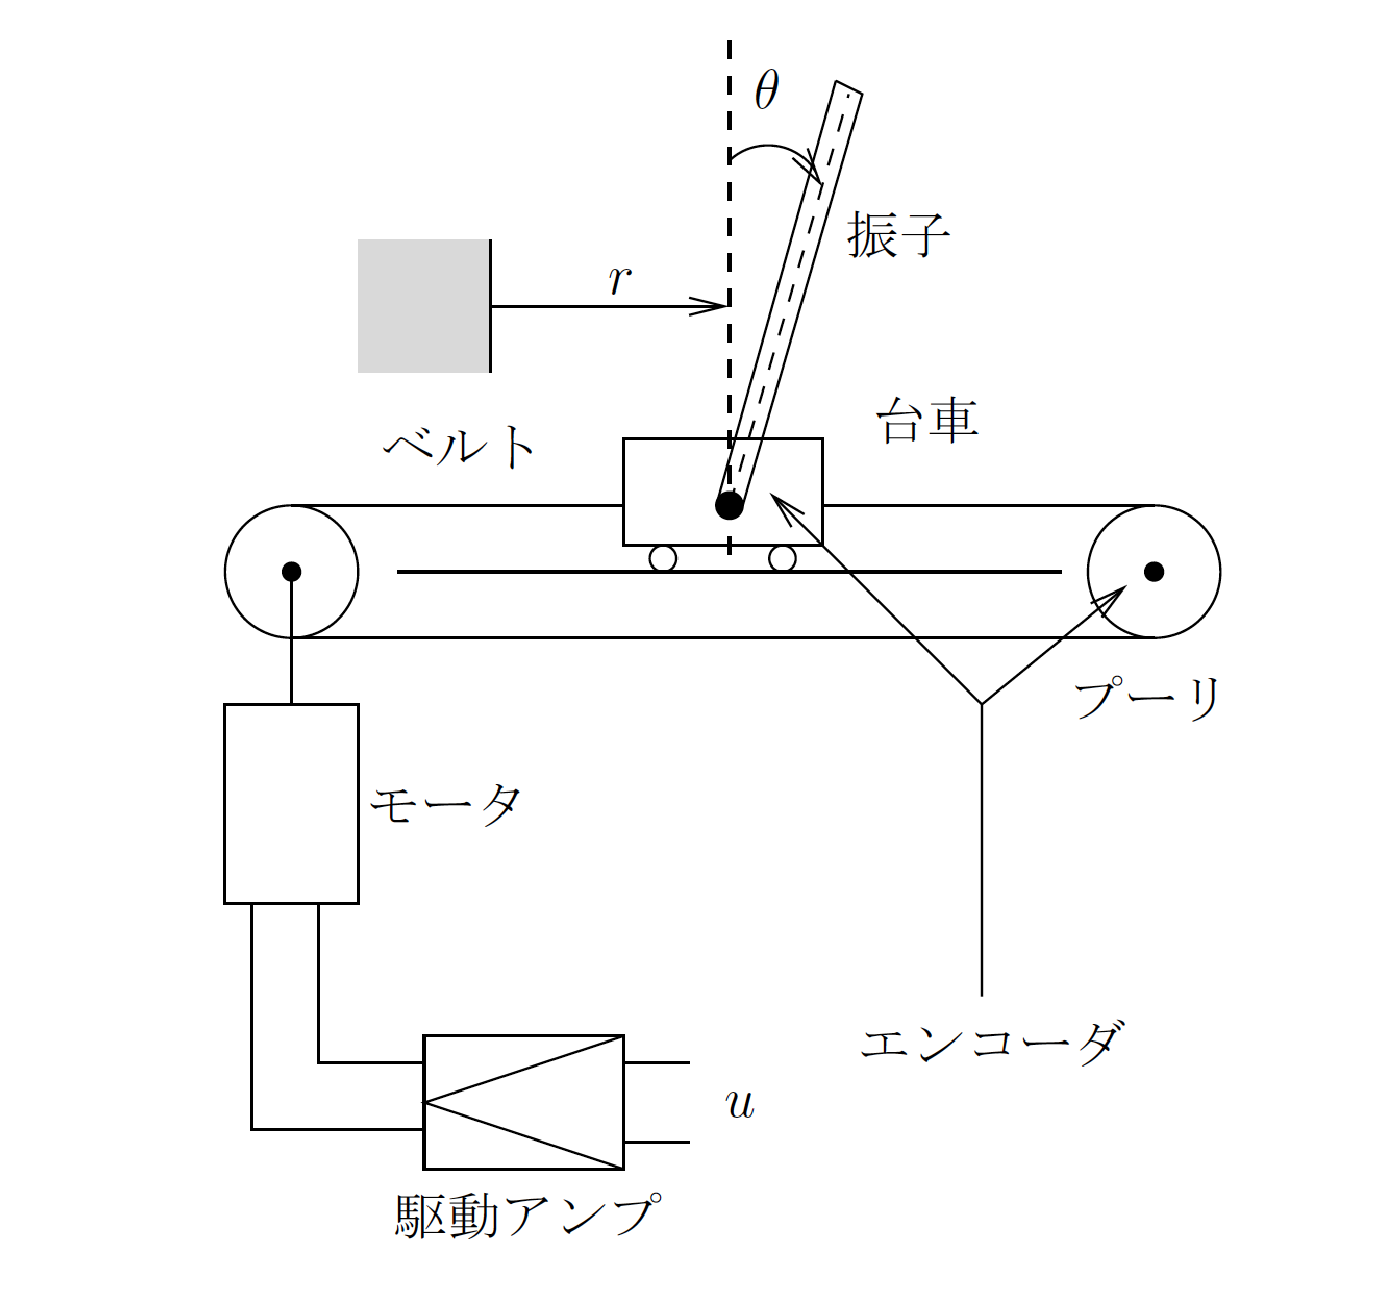
\includegraphics[width = 0.6 \linewidth]{model.eps}
		\caption{倒立振子系}
		\label{fig:倒立振子系}
	\end{center}
\end{figure}

\chapter{モデリング}
\section{数式モデル}
制御目的を達成する制御システムを設計するためにまず、倒立振子系について、状態方程式と観測方程式から成る数式モデルを導出する。
\subsection{状態方程式}
% 2.1図の挿入
\begin{figure}[htbp]
	\begin{center}
		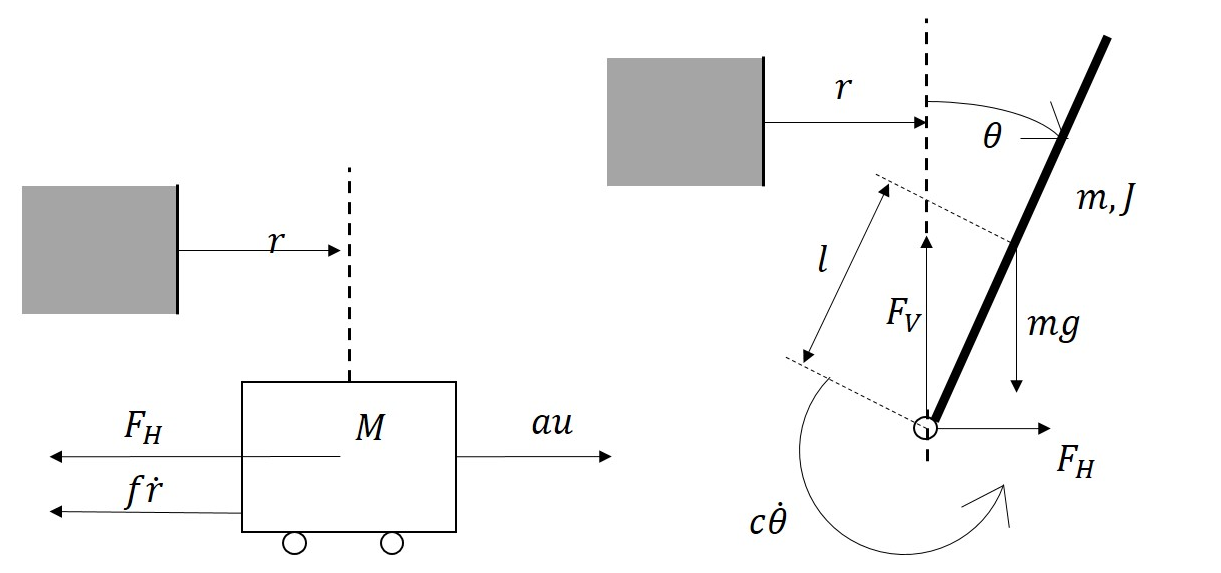
\includegraphics[width = 0.6 \linewidth]{modeling.eps}
		\caption{数学モデル導出のための参考図}
		\label{fig:数式モデル導出のための参考図}
	\end{center}
\end{figure}

図\ref{fig:数式モデル導出のための参考図}を参照して、台車と振子に関する運動方程式がつぎのように得られる。

\begin{eqnarray}
&&M \ddot{r} = au - F_H - f \dot{r}
\label{eq:2.1}\\
&&J \ddot{\theta} = lF_V\sin{\theta} - lF_H\cos{\theta} - c\dot{\theta}
\label{eq:2.2}\\
&&m \frac{d^2}{dx^2} (r + l\sin(\theta))  =  F_H
\label{eq:2.3}\\
&&m \frac{d^2}{dx^2} (l\cos(\theta))  =  F_V - mg
\label{eq:2.4}
\end{eqnarray}
ここで、$M,f$は台車の質量と摩擦係数、$m,l,J,c$は振子の質量、回転軸・重心間距離、重心まわり慣性モーメント、回転軸摩擦係数、$F_H,F_V$は振子が台車から受ける水平抗力と垂直抗力である。また、$u$は駆動アンプへの入力電圧、$a$は駆動アンプへの入力電圧から台車への駆動力までのゲインである。

いま、4つの状態変数から成るベクトル、すなわち状態$x$を
\begin{eqnarray}
	x=\left[
	\begin{array}{c}
		r\\
		\theta\\
		\dot{r}\\
		\dot{\theta}
	\end{array}
	\right]
\end{eqnarray}
のように定義すると、、(\ref{eq:2.1})-(\ref{eq:2.4})式から、倒立振子系の非線形状態方程式を求める。
(\ref{eq:2.1})に(\ref{eq:2.2})を代入すると

\begin{eqnarray}
	M\ddot{r} = au - m\ddot{r}+ml\sin{\theta}-f\dot{r}
\end{eqnarray}
\begin{eqnarray}
\ddot{r} = \frac{au + ml\sin{\theta}-f\dot{r}}{M+m}
\label{eq:rddot}
\end{eqnarray}
また、(\ref{eq:2.2})に(\ref{eq:2.3}),(\ref{eq:2.4})を代入すると
\begin{eqnarray}
	J\ddot{\theta} = l\left(m\frac{d^2}{dt^2}(l\cos{\theta}+mg) \right)\sin{\theta}
	- l \left( m\frac{d^2}{dt^2}(r+l\sin{\theta}) \right)\cos{\theta}
\end{eqnarray}
\begin{eqnarray}
ml\cos{\theta}\ddot{r}+(J+ml^2)\ddot(\theta)=mgl\sin{\theta}-c\dot{\theta}
\label{eq:rddot,thddot}
\end{eqnarray}
(\ref{eq:rddot}),(\ref{eq:rddot,thddot})を行列式で表すと
\begin{eqnarray}
	\left[
	\begin{array}{cc}
		M+m & ml\cos{\theta}\\
		ml\cos{\theta} & J+ml^2
	\end{array}
	\right]
	\left[
	\begin{array}{c}
		\ddot{r} \\
		\ddot{\theta}
	\end{array}
	\right] =
	\left[
	\begin{array}{c}
		- f \dot{r} + ml\sin{\theta}\bullet\dot{\theta}^2 + au\\
		mgl\sin{\theta} - c\dot{\theta}
	\end{array}
	\right]\\
	\left[
	\begin{array}{c}
		\ddot{r} \\
		\ddot{\theta}
	\end{array}
	\right] =
	\left[
	\begin{array}{cc}
		M+m & ml\cos{\theta}\\
		ml\cos{\theta} & J+ml^2
	\end{array}
	\right]^{-1}
	\left[
	\begin{array}{c}
		- f \dot{r} + ml\sin{\theta}\bullet\dot{\theta}^2 + au\\
		mgl\sin{\theta} - c\dot{\theta}
	\end{array}
	\right]
\end{eqnarray}
よって、
%(5)
\begin{eqnarray}
\dot{x}=f(x,u)=\left[
\begin{array}{c}

\dot{r}\\
\dot{\theta}\\
K^{-1}\left[
\begin{array}{c}
- f \dot{r} + ml\sin{\theta}\bullet\dot{\theta}^2 + au\\
mgl\sin{\theta} - c\dot{\theta}
\end{array}
\right]

\end{array}
\right],\,
K = \left[
\begin{array}{cc}
M+m & ml\cos{\theta}\\
ml\cos{\theta} & J+ml^2
\end{array}
\right]
\end{eqnarray}
のように得られる。

ところで、倒立振子系については、その制御目的から、不安定平衡点$x=0$の近傍での挙動を表す方程式を知れば充分である。そこで、この基準状態まわりで一次近似された状態方程式を求めることを考える

倒立振子系に対する状態方程式は、つぎのように得られる。
%(6)
\begin{eqnarray}
\dot{x} = Ax + Bu
\label{eq:xdot}
\end{eqnarray}
ここで

\begin{eqnarray}
	A = \left[
	\begin{array}{cc}
		0_{2\times2} & I_2\\
		A_{21} & A_{22}
	\end{array}
	\right],\,
	B = \left[
	\begin{array}{c}
		0_{2\times2}\\
		B_2
	\end{array}
	\right]\\
\end{eqnarray}
ただし

\begin{eqnarray}
	A_{21} = K^{-1}\left[
	\begin{array}{cc}
		0 &  0 \\
		0 & mgl
	\end{array}
	\right],\,
	A_{22} = K^{-1}\left[
	\begin{array}{cc}
		-f &  0 \\
		0 & -c
	\end{array}
	\right],\,
	B_{2} = K^{-1}\left[
	\begin{array}{c}
		a\\
		0
	\end{array}
	\right]
\end{eqnarray}

\begin{eqnarray}
	K = \left[
	\begin{array}{cc}
		M+m & ml \\
		ml & J+ml^2
	\end{array}
	\right]
\end{eqnarray}

\subsection{観測方程式}
2つの観測出力は
\begin{eqnarray}
	y_1 = c_1r\\
	y_2 = c_2\theta
\end{eqnarray}
のように表される。ここで$c_1$は変位・電圧変換係数、$c_2$は角度・電圧変換係数である。これから成るベクトルすなわち出力$y$を

\begin{eqnarray}
	y = \left[
	\begin{array}{c}
		y_1\\
		y_2
	\end{array}
	\right]
\end{eqnarray}
のように定義すると、倒立振子系に対する観測方程式として

\begin{eqnarray}
	y = Cx
\end{eqnarray}
ただし

\begin{eqnarray}
C = \left[
\begin{array}{cc}
N & 0_{2\times2}
\end{array}
\right] = \left[
\begin{array}{cccc}
c_1 &  0  & 0 & 0\\
0  & c_2 & 0 & 0
\end{array}
\right],\,
N = \left[
\begin{array}{cc}
c_1 &  0 \\
0  & c_2
\end{array}
\right]
\label{eq:C,N}
\end{eqnarray}
を得る。
=======
	\section{実験目的}
		本実験の目的は倒立振子の安定化制御の制御系の設計を状態空間法を用いて行うことにより、線形時不変システムに対する設計法を習得することである。
	\section{制御対象と制御目的}
		\subsection{倒立振子系}
			制御対象として、図\ref{fig:倒立振子系}に示されるような倒立振子系を考える。モノレール上に台車が置かれ、台車上のモノレールと直角な軸に一本の棒が取り付けられ、棒はその軸まわりに自由に回転できる。台車はベルトとプーリを介して、モータにより駆動され、モノレール上を走行できる。すなわち、棒(振子)は鉛直線とモノレールにより定まる平面に拘束されて、台車によって動かされるようになっている。

		\subsection{観測出力と操作入力}
			倒立振子系の観測出力として、ポテンショメータにより、次の2つが測定できる。
			\begin{description}
				\setlength{\itemindent}{0pt}
				\item[1°] 台車の基準位置からの変位$r$に比例する電圧$y_1$
				\item[2°] 棒の鉛直線となす角度$\theta$に比例する電圧$y_2$
			\end{description}
			一方、操作入力は、つぎのものである。
			\begin{description}
			\setlength{\itemindent}{0pt}
			\item[1°] モータの駆動アンプへの入力電圧$u$
			\end{description}
			ここで、モータにより駆動される台車には、$u$に比例した駆動力が働くものとする。

		\subsection{制御目的}
			この倒立振子系は、2つの平衡点をもつ。1つは棒が鉛直線に沿って垂れ下がった状態、もう一つは棒が鉛直線に沿って倒立した状態である。前者は、棒を揺らせば、いわゆる振子となり、揺らせれば、いわゆる振子となり、ゆれは時間が立てば止まるので、安定平衡点である。後者は、いわゆる倒立振子であるが、倒立状態にある棒を少しでもつつけば、真っ逆さまに落ちていくので、不安定平衡点である。このような倒立振子系に対する制御目的として、つぎを考える。
			\begin{description}
			\setlength{\itemindent}{0pt}
			\item[1゜]倒立状態にある棒が何らかの原因で傾いたとき、台車を動かして、棒をすみやかに倒立状態に戻す(不安定抵抗店の安定化)。
			\item[2゜]倒立位置を指定した位置に移動させる。
			\end{description}
			% 1.1図の挿入
			\begin{figure}[htbp]
				\begin{center}
					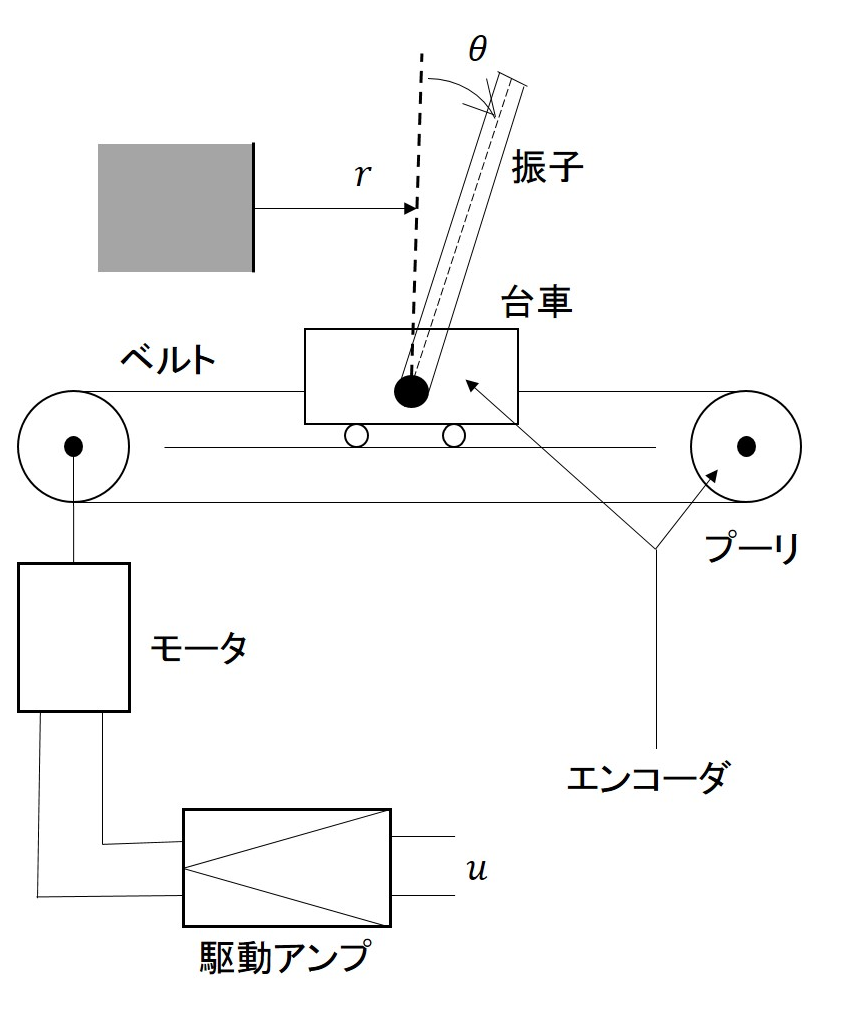
\includegraphics[width = 0.6 \linewidth]{pendulum.eps}
					\caption{倒立振子系}
					\label{fig:倒立振子系}
				\end{center}
			\end{figure}

\chapter{モデリング}
=======
	\section{実験目的}
		本実験の目的は倒立振子の安定化制御の制御系の設計を状態空間法を用いて行うことにより、線形時不変システムに対する設計法を習得することである。
	\section{制御対象と制御目的}
		\subsection{倒立振子系}
			制御対象として、図\ref{fig:倒立振子系}に示されるような倒立振子系を考える。モノレール上に台車が置かれ、台車上のモノレールと直角な軸に一本の棒が取り付けられ、棒はその軸まわりに自由に回転できる。台車はベルトとプーリを介して、モータにより駆動され、モノレール上を走行できる。すなわち、棒(振子)は鉛直線とモノレールにより定まる平面に拘束されて、台車によって動かされるようになっている。

		\subsection{観測出力と操作入力}
			倒立振子系の観測出力として、ポテンショメータにより、次の2つが測定できる。
			\begin{description}
				\setlength{\itemindent}{0pt}
				\item[1°] 台車の基準位置からの変位$r$に比例する電圧$y_1$
				\item[2°] 棒の鉛直線となす角度$\theta$に比例する電圧$y_2$
			\end{description}
			一方、操作入力は、つぎのものである。
			\begin{description}
			\setlength{\itemindent}{0pt}
			\item[1°] モータの駆動アンプへの入力電圧$u$
			\end{description}
			ここで、モータにより駆動される台車には、$u$に比例した駆動力が働くものとする。

		\subsection{制御目的}
			この倒立振子系は、2つの平衡点をもつ。1つは棒が鉛直線に沿って垂れ下がった状態、もう一つは棒が鉛直線に沿って倒立した状態である。前者は、棒を揺らせば、いわゆる振子となり、揺らせれば、いわゆる振子となり、ゆれは時間が立てば止まるので、安定平衡点である。後者は、いわゆる倒立振子であるが、倒立状態にある棒を少しでもつつけば、真っ逆さまに落ちていくので、不安定平衡点である。このような倒立振子系に対する制御目的として、つぎを考える。
			\begin{description}
			\setlength{\itemindent}{0pt}
			\item[1゜]倒立状態にある棒が何らかの原因で傾いたとき、台車を動かして、棒をすみやかに倒立状態に戻す(不安定抵抗店の安定化)。
			\item[2゜]倒立位置を指定した位置に移動させる。
			\end{description}
			% 1.1図の挿入
			\begin{figure}[htbp]
				\begin{center}
					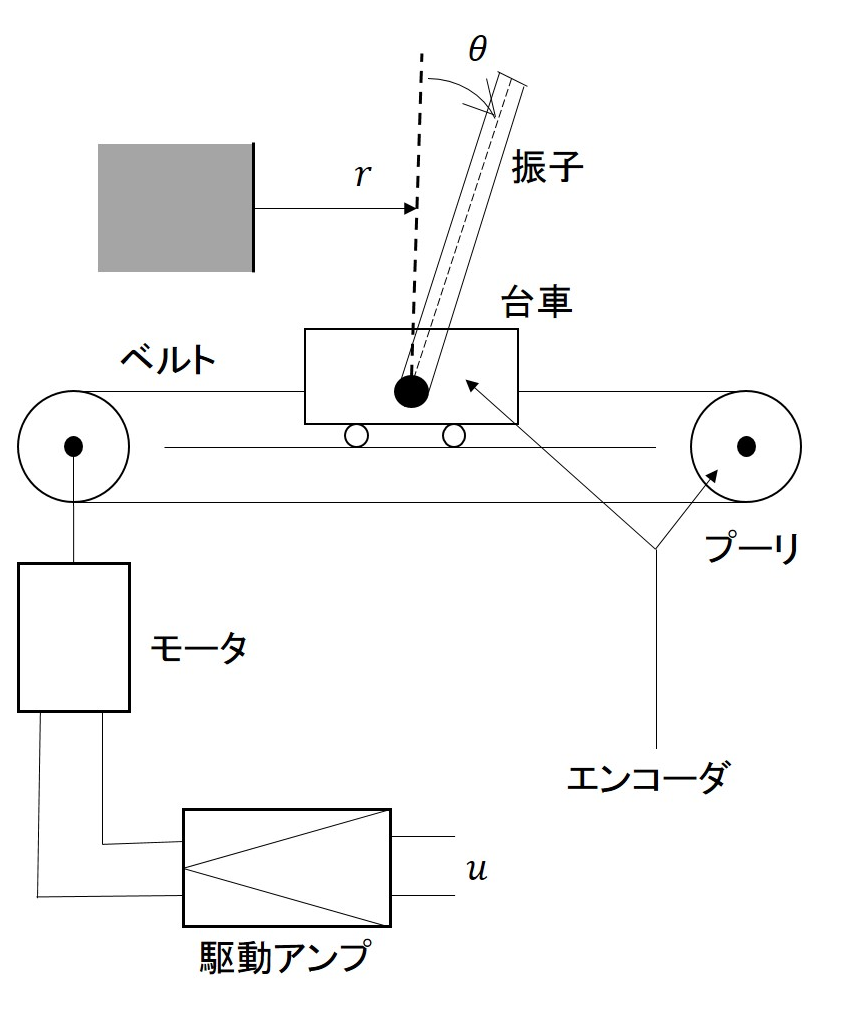
\includegraphics[width = 0.6 \linewidth]{pendulum.eps}
					\caption{倒立振子系}
					\label{fig:倒立振子系}
				\end{center}
			\end{figure}

\chapter{モデリング}
>>>>>>> 1393f4f07a5b2b89c455e47e2d9b68edaf40a925
	\section{数式モデル}
		制御目的を達成する制御システムを設計するためにまず、倒立振子系について、状態方程式と観測方程式から成る数式モデルを導出する。
		\subsection{状態方程式}
			% 2.1図の挿入
			\begin{figure}[htbp]
				\begin{center}
					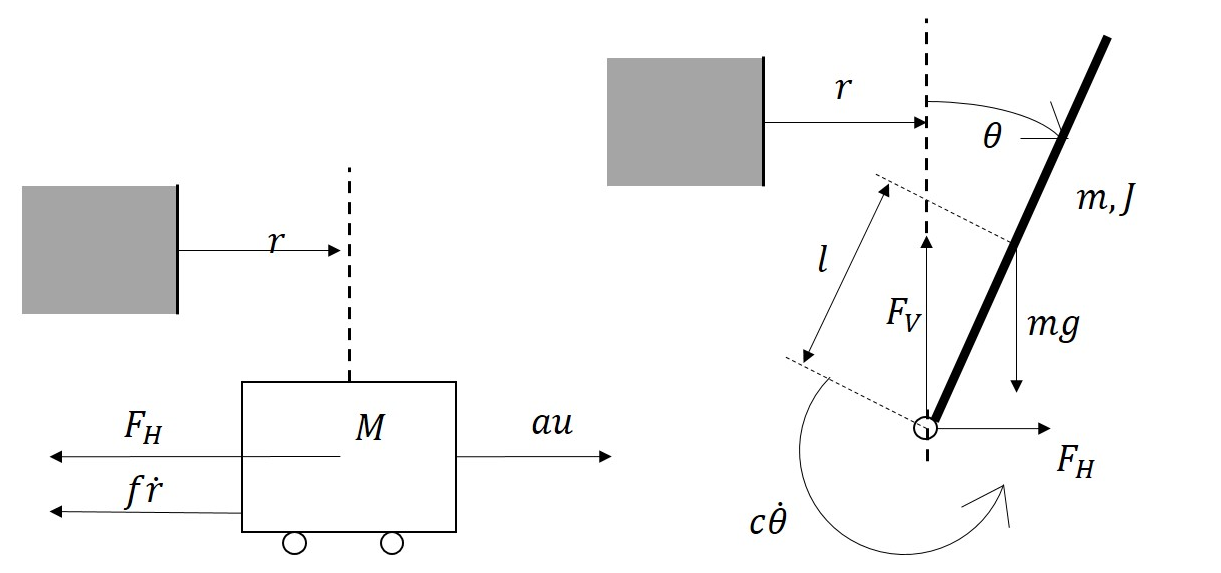
\includegraphics[width = 0.6 \linewidth]{modeling.eps}
					\caption{数学モデル導出のための参考図}
					\label{fig:数式モデル導出のための参考図}
				\end{center}
			\end{figure}

			図\ref{fig:数式モデル導出のための参考図}を参照して、台車と振子に関する運動方程式がつぎのように得られる。

			\begin{eqnarray}
			&&M \ddot{r} = au - F_H - f \dot{r}
			\label{eq:2.1}\\
			&&J \ddot{\theta} = lF_V\sin{\theta} - lF_H\cos{\theta} - c\dot{\theta}
			\label{eq:2.2}\\
			&&m \frac{d^2}{dx^2} (r + l\sin{\theta})  =  F_H
			\label{eq:2.3}\\
			&&m \frac{d^2}{dx^2} (l\cos{\theta})  =  F_V - mg
			\label{eq:2.4}
			\end{eqnarray}
			ここで、$M,f$は台車の質量と摩擦係数、$m,l,J,c$は振子の質量、回転軸・重心間距離、重心まわり慣性モーメント、回転軸摩擦係数、$F_H,F_V$は振子が台車から受ける水平抗力と垂直抗力である。また、$u$は駆動アンプへの入力電圧、$a$は駆動アンプへの入力電圧から台車への駆動力までのゲインである。

			いま、4つの状態変数から成るベクトル、すなわち状態$x$を
			\begin{eqnarray*}
				x=\left[
				\begin{array}{c}
					r\\
					\theta\\
					\dot{r}\\
					\dot{\theta}
				\end{array}
				\right]
			\end{eqnarray*}
			のように定義し、(\ref{eq:2.1})-(\ref{eq:2.4})式から、倒立振子系の非線形状態方程式を求める。
			(\ref{eq:2.1})に(\ref{eq:2.3})を代入すると

			\begin{eqnarray*}
				M\ddot{r} = au - m\ddot{r}+ml\sin{\theta} ・ {\dot{\theta}}^2 - ml\cos{\theta}・\ddot{\theta}-f\dot{r}
			\end{eqnarray*}
			\begin{eqnarray}
			\left( M+m \right) \ddot{r} + ml\cos{\theta}・\ddot{\theta} = au + ml\sin{\theta} ・ {\dot{\theta}}^2-f\dot{r}
			\label{eq:rddot}
			\end{eqnarray}
			また、(\ref{eq:2.2})に(\ref{eq:2.3}),(\ref{eq:2.4})を代入すると
			\begin{eqnarray*}
				J\ddot{\theta} = l\left\lbrace  m\frac{d^2}{dt^2}\left(l\cos{\theta}+mg\right) \right\rbrace\sin{\theta}
				- l \left\lbrace m\frac{d^2}{dt^2}(r+l\sin{\theta}) \right\rbrace\cos{\theta}-c\dot{\theta}
			\end{eqnarray*}
			\begin{eqnarray}
				(J+ml^2)\ddot{\theta}=mgl\sin{\theta}-ml\cos{\theta}・\ddot{r}-c\dot{\theta}
				\label{eq:rddot,thddot}
			\end{eqnarray}
			(\ref{eq:rddot}),(\ref{eq:rddot,thddot})を行列式で表すと
			\begin{eqnarray*}
				\left[
					\begin{array}{cc}
						M+m & ml\cos{\theta}\\
						ml\cos{\theta} & J+ml^2
					\end{array}
				\right]
				\left[
					\begin{array}{c}
						\ddot{r} \\
						\ddot{\theta}
					\end{array}
				\right] 
				=
				\left[
					\begin{array}{c}
<<<<<<< HEAD
						- f \dot{r} + ml\sin{\theta}\bullet\dot{\theta}^2 + au\\
=======
						- f \dot{r} + ml\sin{\theta}・\dot{\theta}^2 + au\\
>>>>>>> 1393f4f07a5b2b89c455e47e2d9b68edaf40a925
						mgl\sin{\theta} - c\dot{\theta}
					\end{array}
				\right]
			\end{eqnarray*}
			\begin{eqnarray*}
				\left[
					\begin{array}{c}
						\ddot{r} \\
						\ddot{\theta}
					\end{array}
				\right]
				 =
				\left[
					\begin{array}{cc}
						M+m & ml\cos{\theta}\\
						ml\cos{\theta} & J+ml^2
					\end{array}
				\right]^{-1}
				\left[
					\begin{array}{c}
<<<<<<< HEAD
						- f \dot{r} + ml\sin{\theta}\bullet\dot{\theta}^2 + au\\
=======
						- f \dot{r} + ml\sin{\theta}・\dot{\theta}^2 + au\\
>>>>>>> 1393f4f07a5b2b89c455e47e2d9b68edaf40a925
						mgl\sin{\theta} - c\dot{\theta}
					\end{array}
				\right]
			\end{eqnarray*}
			よって、
			%(5)
			\begin{eqnarray}
				\dot{x}
				=
				f(x,u)
				=
				\left[
					\begin{array}{c}
						\dot{r}\\
						\dot{\theta}\\
						K^{-1}\left[
						\begin{array}{c}
<<<<<<< HEAD
							- f \dot{r} + ml\sin{\theta}\bullet\dot{\theta}^2 + au\\
=======
							- f \dot{r} + ml\sin{\theta}・\dot{\theta}^2 + au\\
>>>>>>> 1393f4f07a5b2b89c455e47e2d9b68edaf40a925
							mgl\sin{\theta} - c\dot{\theta}
						\end{array}
						\right]
					\end{array}
				\right],\,
				K 
				= 
				\left[
					\begin{array}{cc}
						M+m & ml\cos{\theta}\\
						ml\cos{\theta} & J+ml^2
					\end{array}
				\right]
			\end{eqnarray}
			のように得られる。

			ところで、倒立振子系については、その制御目的から、不安定平衡点$x=0$の近傍での挙動を表す方程式を知れば充分である。そこで、この基準状態まわりで一次近似された状態方程式を求めることを考える
			
			倒立振子系に対する状態方程式は、つぎのように得られる。
			%(6)
			\begin{eqnarray}
				\dot{x} = Ax + Bu
				\label{eq:xdot}
			\end{eqnarray}
			ここで

			\begin{eqnarray*}
				A = \left[
				\begin{array}{cc}
<<<<<<< HEAD
					0_{2\times2} & I_2\\
=======
					0_{2×2} & I_2\\
>>>>>>> 1393f4f07a5b2b89c455e47e2d9b68edaf40a925
					A_{21} & A_{22}
				\end{array}
				\right],\,
				B = \left[
				\begin{array}{c}
<<<<<<< HEAD
					0_{2\times2}\\
=======
					0_{2×2}\\
>>>>>>> 1393f4f07a5b2b89c455e47e2d9b68edaf40a925
					B_2
				\end{array}
				\right]
			\end{eqnarray*}
			ただし

			\begin{eqnarray*}
				A_{21} = K^{-1}\left[
				\begin{array}{cc}
					0 &  0 \\
					0 & mgl
				\end{array}
				\right],\,
				A_{22} = K^{-1}\left[
				\begin{array}{cc}
					-f &  0 \\
					0 & -c
				\end{array}
				\right]
				,\,
				B_{2} = K^{-1}\left[
				\begin{array}{c}
					a\\
					0
				\end{array}
				\right]
				\nonumber
			\end{eqnarray*}

			\begin{eqnarray*}
				K = \left[
				\begin{array}{cc}
					M+m & ml \\
					ml & J+ml^2
				\end{array}
				\right]
			\end{eqnarray*}

	\subsection{観測方程式}
	2つの観測出力は
	\begin{eqnarray*}
		y_1 = c_1r\\
		y_2 = c_2\theta
	\end{eqnarray*}
	のように表される。ここで$c_1$は変位・電圧変換係数、$c_2$は角度・電圧変換係数である。これから成るベクトルすなわち出力$y$を

	\begin{eqnarray*}
		y = \left[
		\begin{array}{c}
			y_1\\
			y_2
		\end{array}
		\right]
	\end{eqnarray*}
	のように定義すると、倒立振子系に対する観測方程式として

	\begin{eqnarray*}
		y = Cx
	\end{eqnarray*}
	ただし

	\begin{eqnarray}
		C 
		= 
		\left[
			\begin{array}{cc}
<<<<<<< HEAD
				N & 0_{2\times2}
=======
				N & 0_{2×2}
>>>>>>> 1393f4f07a5b2b89c455e47e2d9b68edaf40a925
			\end{array}
		\right] 
		=
		\left[
			\begin{array}{cccc}
				c_1 &  0  & 0 & 0\\
				0  & c_2 & 0 & 0
			\end{array}
		\right],\,
		N 
		=
		\left[
			\begin{array}{cc}
				c_1 &  0 \\
				0  & c_2
			\end{array}
		\right]
		\label{eq:C,N}
	\end{eqnarray}
	を得る。
<<<<<<< HEAD
>>>>>>> c75b7fa605d82ac36c3c13370dbdcf9029f17b03
=======
>>>>>>> 1393f4f07a5b2b89c455e47e2d9b68edaf40a925

\section{物理パラメータの決定}
	\subsection{$m$と$l$の測定}
	振子を装置から取り外し、バネ秤で$m$を測定しなさい。つぎに、振子を鋼尺のエッジ上で
	バランスさせて、重心の位置を定め、$l$を測定する。

	\subsection{$c_1$と$c_2$の測定}
	$c_1$と$c_2$は、
	\begin{eqnarray*}
		c_1 = 1.0\\
		c_2 = 1.0
	\end{eqnarray*}
	のようにソフトウェア内で設定済みである。

	\subsection{$a$の測定}
	モータに一定電圧を加え、バネばかりで台車を引き、台車が正の方向に動き出すときの力($au+摩擦力$)を$f_{max}$、負の方向に動き出すときの力($au+摩擦力$)を$f_{min}$とする。図\ref{fig:パラメータaの決定}にしめすように$u$と$f_{max},f_{min}$の関係をいくつかの電圧について調べ、最小2乗法によって1次関数を求め、この傾きを$a$とする。


	% 2.2図の挿入
	\begin{figure}[htbp]
		\begin{center}
			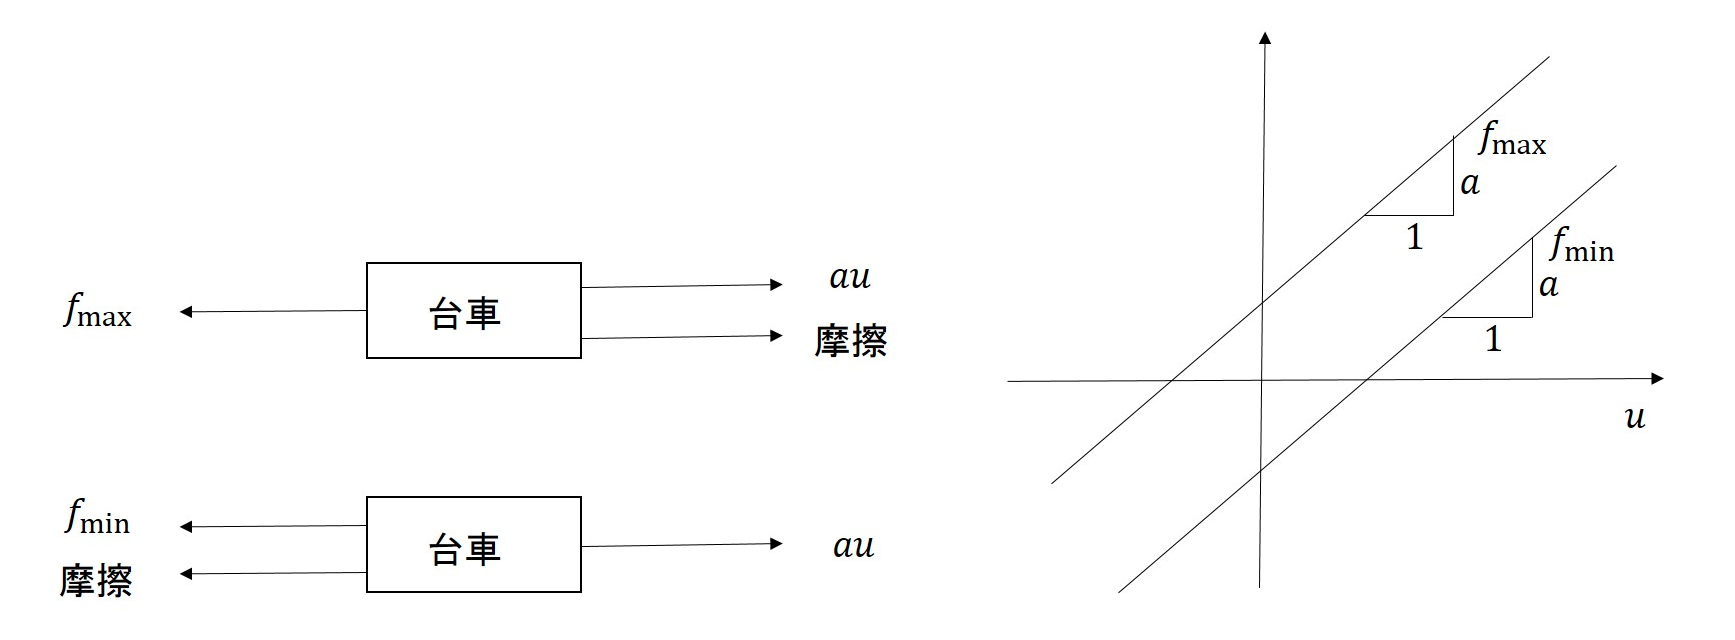
\includegraphics[width = 0.8 \linewidth]{a.eps}
			\caption{パラメータaの決定}
			\label{fig:パラメータaの決定}
		\end{center}
	\end{figure}
<<<<<<< HEAD

	\subsection{ステップ応答による$M$と$f$の測定}

	% 2.3図の挿入
	\begin{figure}[htbp]
		\begin{center}
			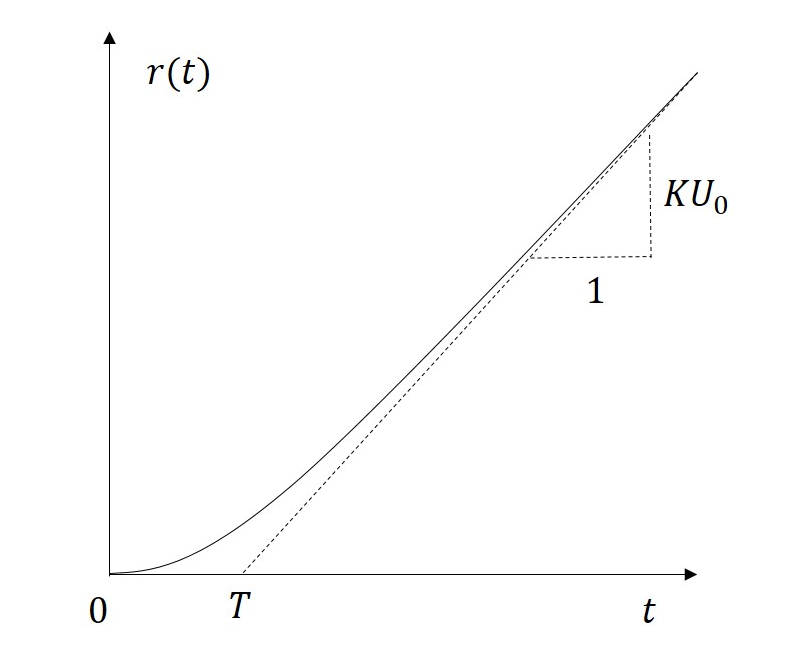
\includegraphics[width = 0.6 \linewidth]{step.eps}
			\caption{台車のステップ応答}
			\label{fig:台車のステップ応答}
		\end{center}
	\end{figure}

	振子を台車から取り外して、台車のステップ応答を測定する。そのときの運動方程式は
	\begin{eqnarray*}
		M\ddot{r} = au - fr
	\end{eqnarray*}
	であり、$u$から$r$までの伝達関数$G$を求めると
	\begin{eqnarray*}
		G(s) = \frac{K}{s(Ts+1)}
	\end{eqnarray*}
	となる。だたし、
	\begin{eqnarray}
		K = \frac{a}{f},T = \frac{M}{f}
		\label{eq:K,T}
	\end{eqnarray}
	である。初期状態をゼロとするとき、このシステムのステップ応答は
	\begin{eqnarray}
		r(t) = KU_o(T\exp{\frac{-t}{T}}+t-T)
		\label{eq:r(t)}
	\end{eqnarray}
	である。(図\ref{fig:台車のステップ応答}参照)。$U_0$はステップの高さである。(\ref{eq:r(t)})式において$t→∞$とすれば
	\begin{eqnarray}
		r(t) = KU_o(t-T)
	\end{eqnarray}
	となり、これから$T$と$K$をもとめ(図\ref{fig:台車のステップ応答}参照)、(\ref{eq:K,T})式より$M$と$f$を決定することができる。

	\subsection{フィードバック制御による$M$と$f$の測定}
	台車は外見は小さいが、台車を手で動かしてみると、かなり重たい。これはモータ(ギア付)の軸のトルクがあるためである。そこで、$M$と$f$は、アンプ・モータ・プーリ・ベルト・台車系の等価質量と等価摩擦係数として計測する。

	\begin{figure}[htbp]
		\begin{center}
			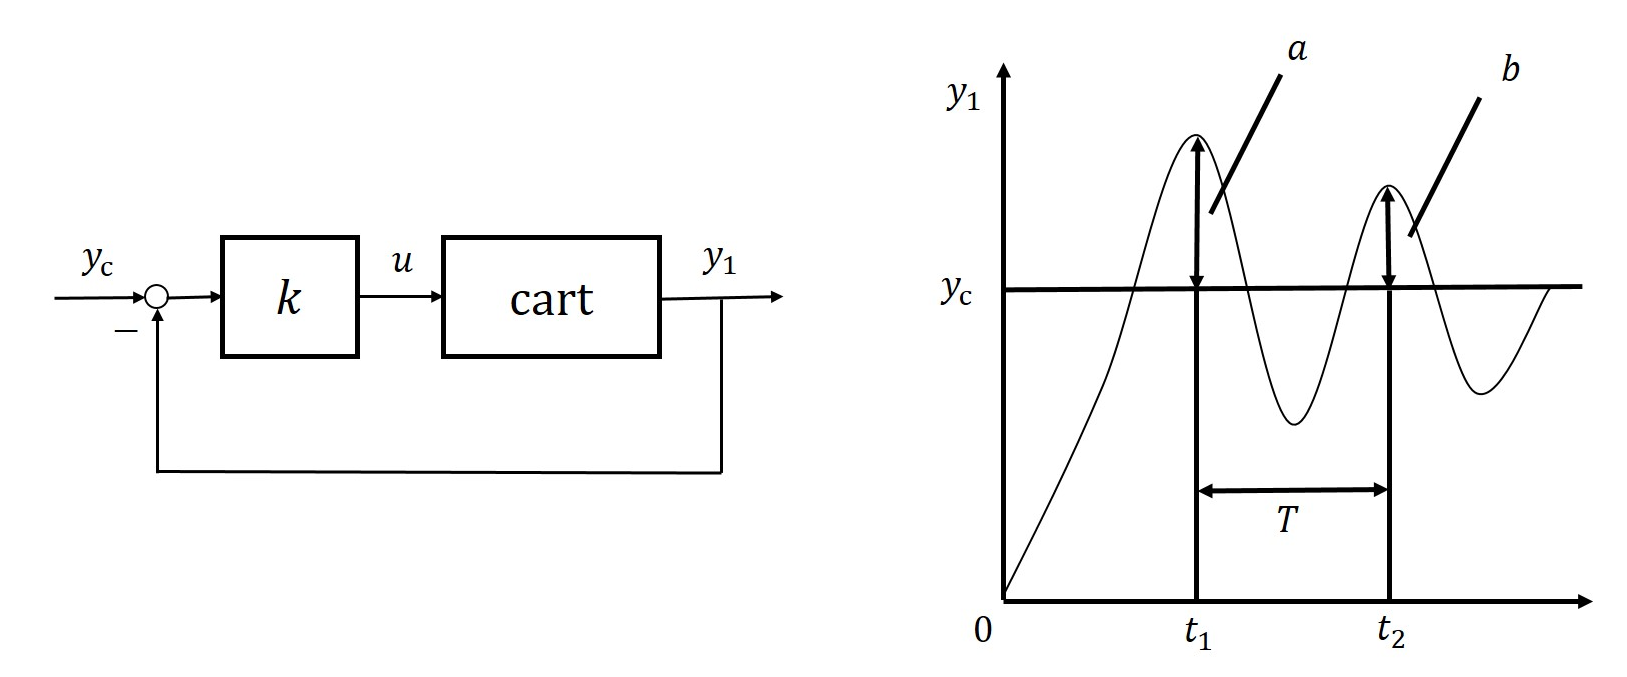
\includegraphics[width=1.0\linewidth]{feedback.eps}
			\caption{台車のフィードバック応答}
			\label{fig:台車のフィードバック応答}
		\end{center}
	\end{figure}

	台車の数式モデルは
	\begin{eqnarray*}
		M\ddot{r} & = & au - fr \\
		y_1 & = & c_1r
	\end{eqnarray*}
	である。これに図\ref{fig:台車のフィードバック応答}に示すようにフィードバック
	\begin{eqnarray*}
		u = k(y_c - y_1)
	\end{eqnarray*}
	を施すと$(y_cは定数,k>0)$、閉ループシステムの応答は
	\begin{eqnarray*}
		M\ddot{y}_1 + f\dot{y}_1 + c_1aky_1 = c_1aky_c
	\end{eqnarray*}
	に従う。一方、偏差$z$を
	
	\begin{eqnarray*}
		z = y_1 - y_c
	\end{eqnarray*}
	により定義すると、これは
	\begin{eqnarray*}
		\ddot{z} + 2\zeta\omega_n\dot{z} + \omega_n^2z = 0
	\end{eqnarray*}
	ただし
	\begin{eqnarray}
		\zeta = \frac{f}{2\sqrt{c_1akM}} , \omega_n = \sqrt{\frac{c_1ak}{M}}
		\label{eq:ZETA,OMEGA}
	\end{eqnarray}
	に従う。この解は
	\begin{eqnarray*}
		0 < \zeta < 1
	\end{eqnarray*}
	このとき、減衰振動となり
	\begin{eqnarray*}
		z(t) = \frac{z_0}{\sqrt{1-\zeta^2}}\exp(-\omega_n\zeta
		t)\,\sin(\omega_n\sqrt{1-\zeta^2}\,t+\phi)
	\end{eqnarray*}
	ただし
	\begin{eqnarray*}
		\phi = \tan^{-1}{\frac{\sqrt{1-\zeta^2}}{\zeta}}
	\end{eqnarray*}
	で与えられる。ここで、$z_0 = z(0) = -y_c$である。いま、$T$とし、
	時刻$t_1$と$t_2 = t_1 + T$において波形$z$の山が隣合うものとする。
	このときの振幅の減衰比は
	\begin{eqnarray*}
		\frac{|z_2(t_2)|}{|z_2(t_1)|} = \exp(-\lambda)
	\end{eqnarray*}
	ただし
	\begin{eqnarray}
		\lambda = \frac{2\pi\zeta}{\sqrt{1-\zeta^2}}
		\label{eq:LAMBDA}
	\end{eqnarray}
	となる。この$\lambda$は対数減衰比と呼ばれる。また
	\begin{eqnarray}
		T = \frac{2\pi}{\omega_n\sqrt{1-\zeta^2}}
		\label{eq:T}
	\end{eqnarray}
	が成り立つ。したがって、(\ref{eq:ZETA,OMEGA})と(\ref{eq:LAMBDA}),(\ref{eq:T})から、$M$と$f$は
	\begin{eqnarray}
		M = \frac{c_1akT^2}{4\pi^2 + \lambda^2},f = \frac{2\lambda M}{T}
		\label{M,f}
	\end{eqnarray}
	のように与えられる。

	\subsection{$J$と$c$の測定}
	振子を自由振動させることにより、$J$と$c$を測定できる。その数式モデルは
	\begin{eqnarray}
		(J+ml^2)\ddot{\theta} & = & -mgl\sin{\theta} - c\dot{\theta}
		\label{eq:J,c1}\\
		y_2 & = & c_2\theta
		\label{eq:J,c2}
	\end{eqnarray}
	で与えられる。$\theta$を微小範囲で考えると、(\ref{eq:J,c1})-(\ref{eq:J,c2})式は
	\begin{eqnarray*}
		\ddot{y}_2 + 2\zeta\omega_n\dot{y_2} + \omega_n^2y_2 = 0
	\end{eqnarray*}
	ただし
	\begin{eqnarray*}
		\zeta = \frac{c}{2\sqrt{mgl(J + ml^2)}},\,
		\omega_n = \sqrt{\frac{mgl}{J + ml^2}}
	\end{eqnarray*}
	のように書くことができる。この解で表される減衰振動の対数減衰率を$\lambda$、周期を$T$とすると、
	関係式(\ref{eq:LAMBDA}),(\ref{eq:T})が成り立つことから、$J,c$は
	\begin{eqnarray}
		J = \frac{mglT_2^2}{4\pi^2 + \lambda^2} - ml^2 ,\, c = \frac{2\lambda(J +
		ml^2)}{T}
	\end{eqnarray}
	のように与えられる。

	\begin{figure}[htbp]
		\begin{center}
			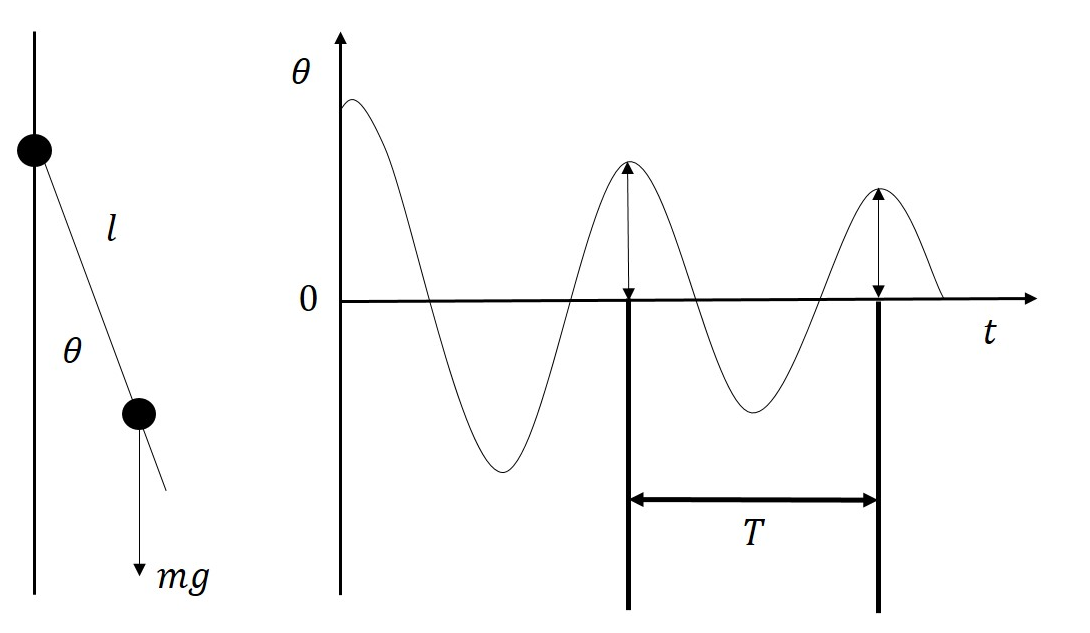
\includegraphics[width = 0.7 \linewidth]{freePend.eps}
			\caption{振子の自由振動}
			\label{fig:振子の自由振動}
		\end{center}
	\end{figure}

<<<<<<< HEAD
\subsection{$a$の測定}
モータに一定電圧を加え、バネばかりで台車を引き、台車が正の方向に動き出すときの力($au+摩擦力$)を$f_{max}$、負の方向に動き出すときの力($au+摩擦力$)を$f_{min}$とする。図\ref{fig:パラメータaの決定}にしめすように$u$と$f_{max},f_{min}$の関係をいくつかの電圧について調べ、最小2乗法によって1次関数を求め、この傾きを$a$とする。


% 2.2図の挿入
\begin{figure}[htbp]
	\begin{center}
		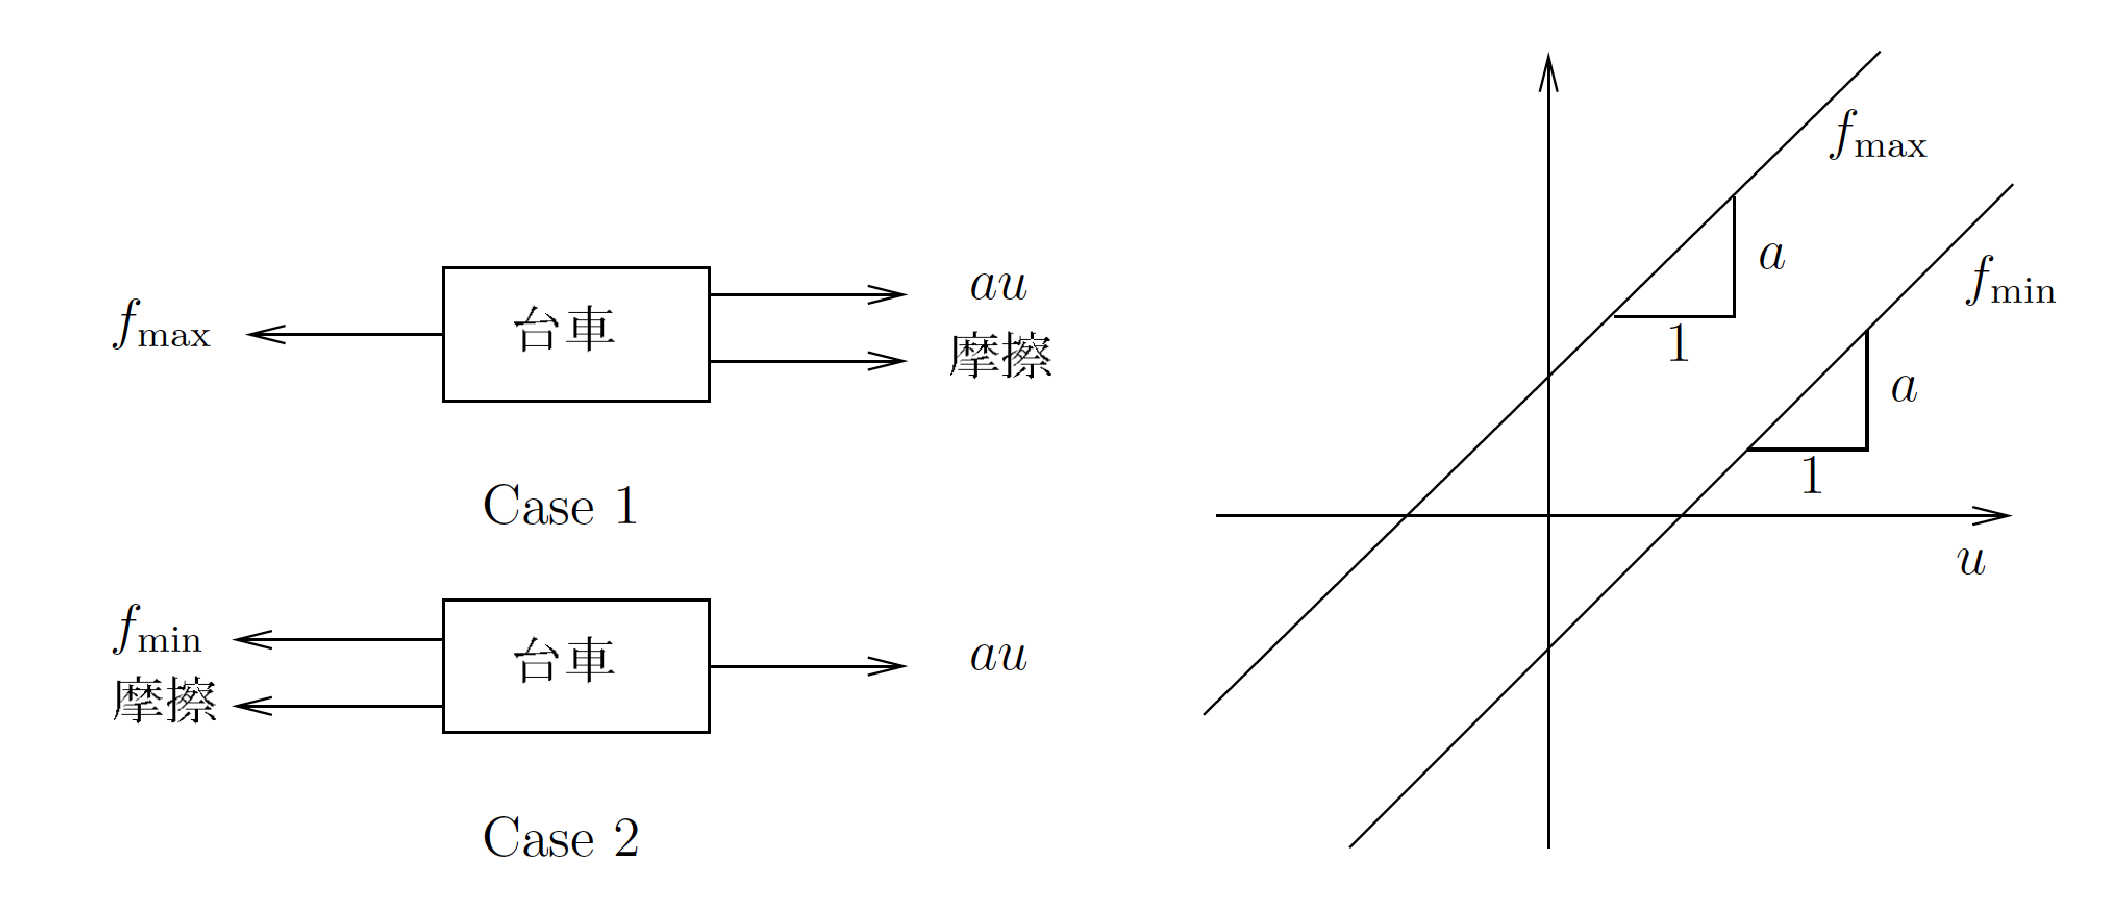
\includegraphics[width = 0.8 \linewidth]{definition_a.eps}
		\caption{パラメータaの決定}
		\label{fig:パラメータaの決定}
	\end{center}
\end{figure}
=======
>>>>>>> c75b7fa605d82ac36c3c13370dbdcf9029f17b03
=======

	\subsection{ステップ応答による$M$と$f$の測定}

	% 2.3図の挿入
	\begin{figure}[htbp]
		\begin{center}
			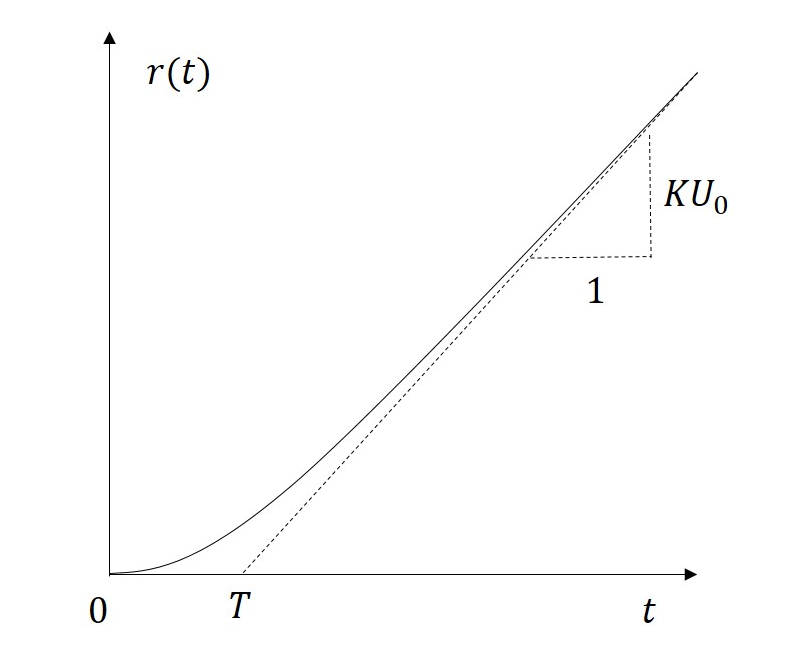
\includegraphics[width = 0.6 \linewidth]{step.eps}
			\caption{台車のステップ応答}
			\label{fig:台車のステップ応答}
		\end{center}
	\end{figure}

	振子を台車から取り外して、台車のステップ応答を測定する。そのときの運動方程式は
	\begin{eqnarray*}
		M\ddot{r} = au - fr
	\end{eqnarray*}
	であり、$u$から$r$までの伝達関数$G$を求めると
	\begin{eqnarray*}
		G(s) = \frac{K}{s(Ts+1)}
	\end{eqnarray*}
	となる。だたし、
	\begin{eqnarray}
		K = \frac{a}{f},T = \frac{M}{f}
		\label{eq:K,T}
	\end{eqnarray}
	である。初期状態をゼロとするとき、このシステムのステップ応答は
	\begin{eqnarray}
		r(t) = KU_o(T\exp{\frac{-t}{T}}+t-T)
		\label{eq:r(t)}
	\end{eqnarray}
	である。(図\ref{fig:台車のステップ応答}参照)。$U_0$はステップの高さである。(\ref{eq:r(t)})式において$t→∞$とすれば
	\begin{eqnarray}
		r(t) = KU_o(t-T)
	\end{eqnarray}
	となり、これから$T$と$K$をもとめ(図\ref{fig:台車のステップ応答}参照)、(\ref{eq:K,T})式より$M$と$f$を決定することができる。

	\subsection{フィードバック制御による$M$と$f$の測定}
	台車は外見は小さいが、台車を手で動かしてみると、かなり重たい。これはモータ(ギア付)の軸のトルクがあるためである。そこで、$M$と$f$は、アンプ・モータ・プーリ・ベルト・台車系の等価質量と等価摩擦係数として計測する。

	\begin{figure}[htbp]
		\begin{center}
			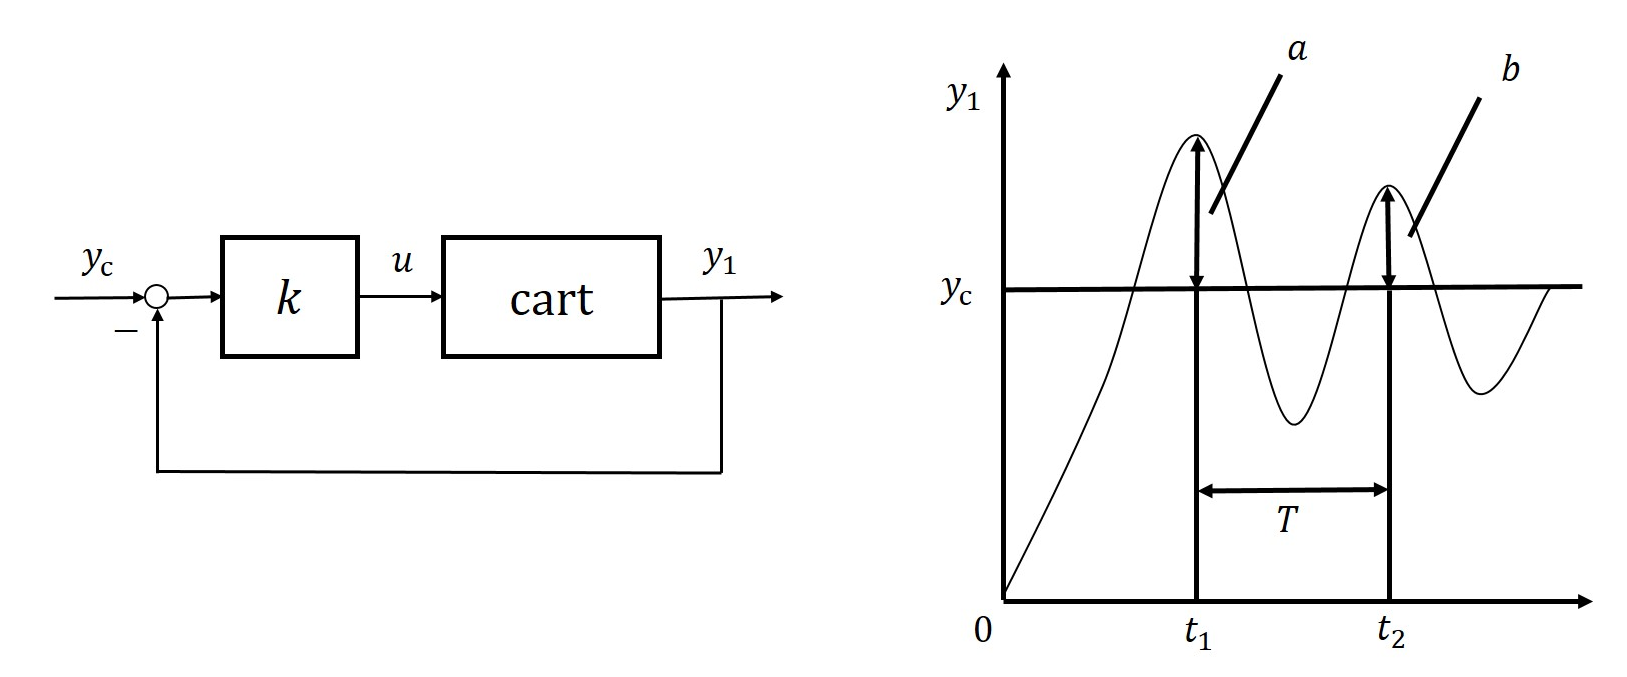
\includegraphics[width=1.0\linewidth]{feedback.eps}
			\caption{台車のフィードバック応答}
			\label{fig:台車のフィードバック応答}
		\end{center}
	\end{figure}

	台車の数式モデルは
	\begin{eqnarray*}
		M\ddot{r} & = & au - fr \\
		y_1 & = & c_1r
	\end{eqnarray*}
	である。これに図\ref{fig:台車のフィードバック応答}に示すようにフィードバック
	\begin{eqnarray*}
		u = k(y_c - y_1)
	\end{eqnarray*}
	を施すと$(y_cは定数,k>0)$、閉ループシステムの応答は
	\begin{eqnarray*}
		M\ddot{y}_1 + f\dot{y}_1 + c_1aky_1 = c_1aky_c
	\end{eqnarray*}
	に従う。一方、偏差$z$を
	
	\begin{eqnarray*}
		z = y_1 - y_c
	\end{eqnarray*}
	により定義すると、これは
	\begin{eqnarray*}
		\ddot{z} + 2\zeta\omega_n\dot{z} + \omega_n^2z = 0
	\end{eqnarray*}
	ただし
	\begin{eqnarray}
		\zeta = \frac{f}{2\sqrt{c_1akM}} , \omega_n = \sqrt{\frac{c_1ak}{M}}
		\label{eq:ZETA,OMEGA}
	\end{eqnarray}
	に従う。この解は
	\begin{eqnarray*}
		0 < \zeta < 1
	\end{eqnarray*}
	このとき、減衰振動となり
	\begin{eqnarray*}
		z(t) = \frac{z_0}{\sqrt{1-\zeta^2}}\exp(-\omega_n\zeta
		t)\,\sin(\omega_n\sqrt{1-\zeta^2}\,t+\phi)
	\end{eqnarray*}
	ただし
	\begin{eqnarray*}
		\phi = \tan^{-1}{\frac{\sqrt{1-\zeta^2}}{\zeta}}
	\end{eqnarray*}
	で与えられる。ここで、$z_0 = z(0) = -y_c$である。いま、$T$とし、
	時刻$t_1$と$t_2 = t_1 + T$において波形$z$の山が隣合うものとする。
	このときの振幅の減衰比は
	\begin{eqnarray*}
		\frac{|z_2(t_2)|}{|z_2(t_1)|} = \exp(-\lambda)
	\end{eqnarray*}
	ただし
	\begin{eqnarray}
		\lambda = \frac{2\pi\zeta}{\sqrt{1-\zeta^2}}
		\label{eq:LAMBDA}
	\end{eqnarray}
	となる。この$\lambda$は対数減衰比と呼ばれる。また
	\begin{eqnarray}
		T = \frac{2\pi}{\omega_n\sqrt{1-\zeta^2}}
		\label{eq:T}
	\end{eqnarray}
	が成り立つ。したがって、(\ref{eq:ZETA,OMEGA})と(\ref{eq:LAMBDA}),(\ref{eq:T})から、$M$と$f$は
	\begin{eqnarray}
		M = \frac{c_1akT^2}{4\pi^2 + \lambda^2},f = \frac{2\lambda M}{T}
		\label{M,f}
	\end{eqnarray}
	のように与えられる。

	\subsection{$J$と$c$の測定}
	振子を自由振動させることにより、$J$と$c$を測定できる。その数式モデルは
	\begin{eqnarray}
		(J+ml^2)\ddot{\theta} & = & -mgl\sin{\theta} - c\dot{\theta}
		\label{eq:J,c1}\\
		y_2 & = & c_2\theta
		\label{eq:J,c2}
	\end{eqnarray}
	で与えられる。$\theta$を微小範囲で考えると、(\ref{eq:J,c1})-(\ref{eq:J,c2})式は
	\begin{eqnarray*}
		\ddot{y}_2 + 2\zeta\omega_n\dot{y_2} + \omega_n^2y_2 = 0
	\end{eqnarray*}
	ただし
	\begin{eqnarray*}
		\zeta = \frac{c}{2\sqrt{mgl(J + ml^2)}},\,
		\omega_n = \sqrt{\frac{mgl}{J + ml^2}}
	\end{eqnarray*}
	のように書くことができる。この解で表される減衰振動の対数減衰率を$\lambda$、周期を$T$とすると、
	関係式(\ref{eq:LAMBDA}),(\ref{eq:T})が成り立つことから、$J,c$は
	\begin{eqnarray}
		J = \frac{mglT_2^2}{4\pi^2 + \lambda^2} - ml^2 ,\, c = \frac{2\lambda(J +
		ml^2)}{T}
	\end{eqnarray}
	のように与えられる。

	\begin{figure}[htbp]
		\begin{center}
			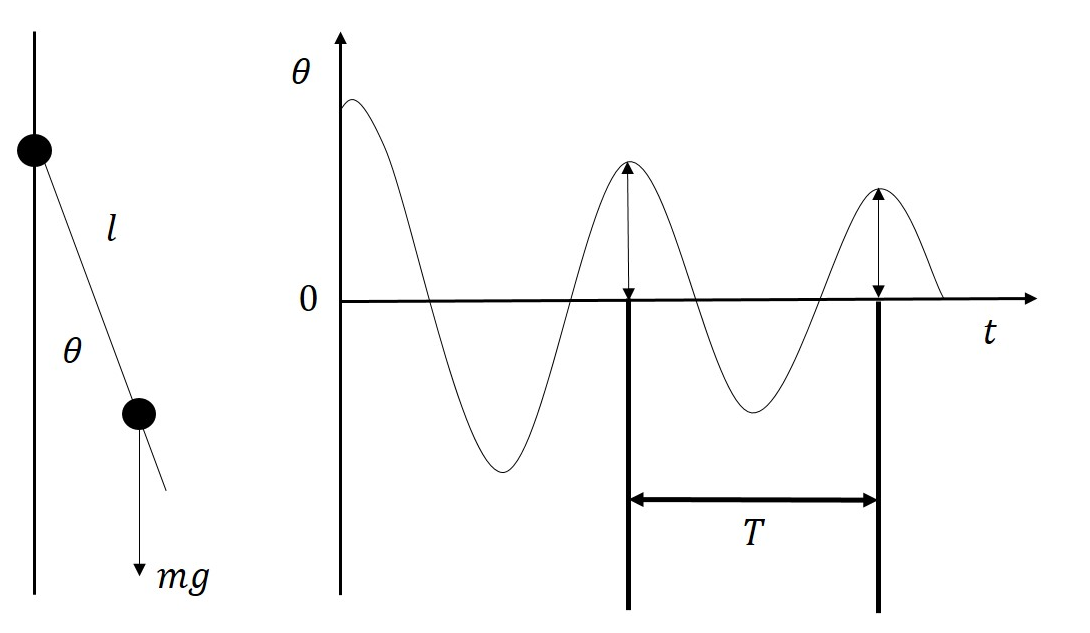
\includegraphics[width = 0.7 \linewidth]{freePend.eps}
			\caption{振子の自由振動}
			\label{fig:振子の自由振動}
		\end{center}
	\end{figure}

>>>>>>> 1393f4f07a5b2b89c455e47e2d9b68edaf40a925

\section{パラメータの検証}
求めたパラメータを以下に示す。

<<<<<<< HEAD
<<<<<<< HEAD
% 2.3図の挿入
\begin{figure}[htbp]
	\begin{center}
		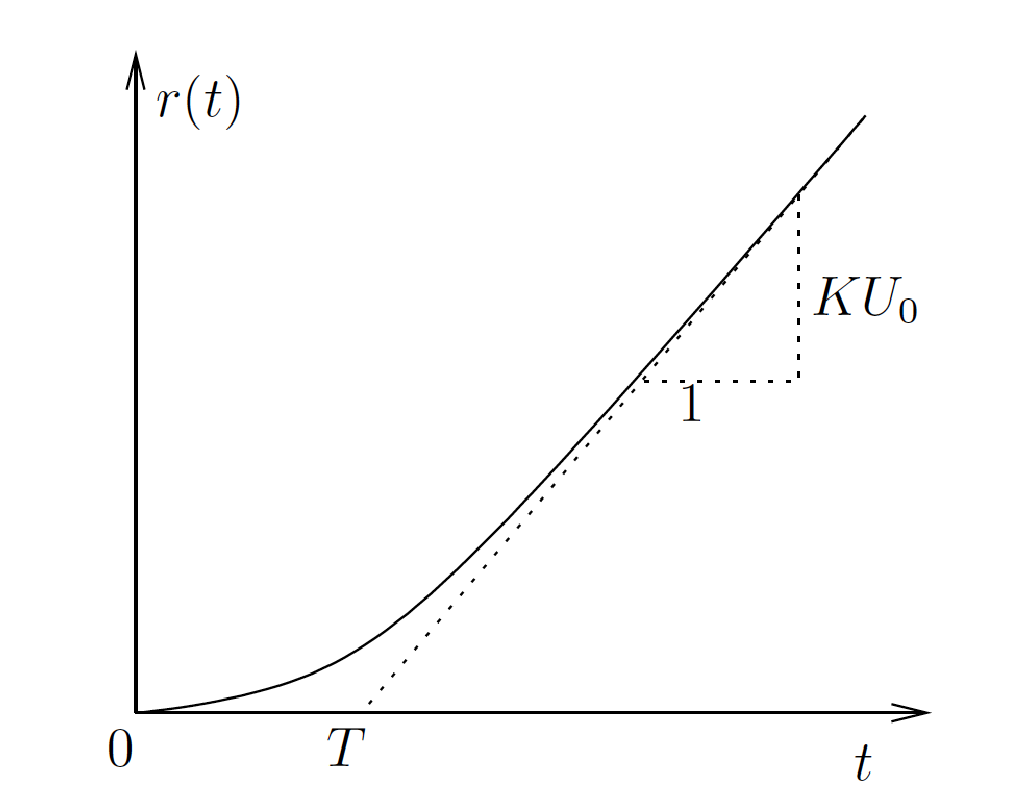
\includegraphics[width = 0.6 \linewidth]{cart_step.eps}
		\caption{台車のステップ応答}
		\label{fig:台車のステップ応答}
	\end{center}
\end{figure}

振子を台車から取り外して、台車のステップ応答を測定する。そのときの運動方程式は
\begin{eqnarray}
	M\ddot{r} = au - fr
\end{eqnarray}
であり、$u$から$r$までの伝達関数$G$を求めると
\begin{eqnarray}
	G(s) = \frac{K}{s(Ts+1)}
\end{eqnarray}
となる。だたし、
\begin{eqnarray}
K = \frac{a}{f},T = \frac{M}{f}
\label{eq:K,T}
\end{eqnarray}
である。初期状態をゼロとするとき、このシステムのステップ応答は
\begin{eqnarray}
r(t) = KU_o(T\exp{\frac{-t}{T}}+t-T)
\label{eq:r(t)}
\end{eqnarray}
である。(図\ref{fig:台車のステップ応答}参照)。$U_0$はステップの高さである。(\ref{eq:r(t)})式において$t→∞$とすれば
\begin{eqnarray}
r(t) = KU_o(t-T)
\end{eqnarray}
となり、これから$T$と$K$をもとめ(図\ref{fig:台車のステップ応答}参照)、(\ref{eq:K,T})式より$M$と$f$を決定することができる。

\subsection{フィードバック制御による$M$と$f$の測定}
台車は外見は小さいが、台車を手で動かしてみると、かなり重たい。これはモータ(ギア付)の軸のトルクがあるためである。そこで、$M$と$f$は、アンプ・モータ・プーリ・ベルト・台車系の等価質量と等価摩擦係数として計測する。

\begin{figure}[htbp]
	\begin{center}
		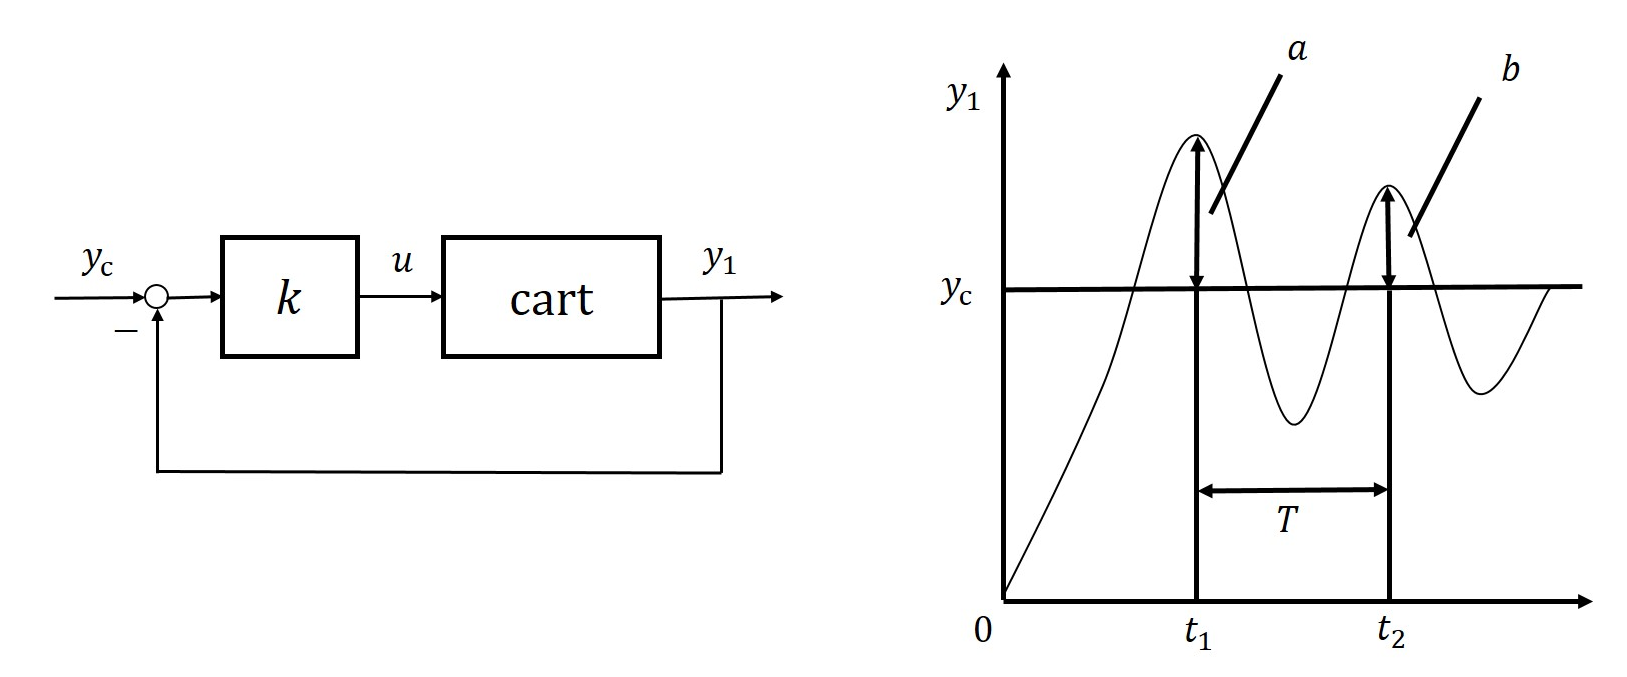
\includegraphics[width = 1.0 \linewidth]{feedback.eps}
		\caption{台車のフィードバック応答}
		\label{fig:台車のフィードバック応答}
	\end{center}
\end{figure}

台車の数式モデルは
\begin{eqnarray}
	M\ddot{r} & = & au - fr \\
	y_1 & = & c_1r
\end{eqnarray}
である。これに図\ref{fig:台車のフィードバック応答}に示すようにフィードバック
\begin{eqnarray}
	u = k(y_c - y_1)
\end{eqnarray}
を施すと$(y_cは定数,k>0)$、閉ループシステムの応答は
\begin{eqnarray}
	M\ddot{y}_1 + f\dot{y}_1 + c_1aky_1 = c_1aky_c
\end{eqnarray}
に従う。一方、偏差$z$を

\begin{eqnarray}
	z = y_1 - y_c
\end{eqnarray}
により定義すると、これは
\begin{eqnarray}
	\ddot{z} + 2\zeta\omega_n\dot{z} + \omega_n^2z = 0
\end{eqnarray}
ただし
\begin{eqnarray}
\zeta = \frac{f}{2\sqrt{c_1akM}} , \omega_n = \sqrt{\frac{c_1ak}{M}}
\label{eq:ZETA,OMEGA}
\end{eqnarray}
に従う。この解は
\begin{eqnarray}
	0 < \zeta < 1
\end{eqnarray}
このとき、減衰振動となり
\begin{eqnarray}
	z(t) = \frac{z_0}{\sqrt{1-\zeta^2}}\exp(-\omega_n\zeta
	t)\,\sin(\omega_n\sqrt{1-\zeta^2}\,t+\phi)
\end{eqnarray}
ただし
\begin{eqnarray}
	\phi = \tan^{-1}{\frac{\sqrt{1-\zeta^2}}{\zeta}}
\end{eqnarray}
で与えられる。ここで、$z_0 = z(0) = -y_c$である。いま、$T$とし、
時刻$t_1$と$t_2 = t_1 + T$において波形$z$の山が隣合うものとする。
このときの振幅の減衰比は
\begin{eqnarray}
	\frac{|z_2(t_2)|}{|z_2(t_1)|} = \exp(-\lambda)
\end{eqnarray}
ただし
\begin{eqnarray}
\lambda = \frac{2\pi\zeta}{\sqrt{1-\zeta^2}}
\label{eq:LAMBDA}
\end{eqnarray}
となる。この$\lambda$は対数減衰比と呼ばれる。また
\begin{eqnarray}
T = \frac{2\pi}{\omega_n\sqrt{1-\zeta^2}}
\label{eq:T}
\end{eqnarray}
が成り立つ。したがって、(\ref{eq:ZETA,OMEGA})と(\ref{eq:LAMBDA}),(\ref{eq:T})から、$M$と$f$は
\begin{eqnarray}
M = \frac{c_1akT^2}{4\pi^2 + \lambda^2},f = \frac{2\lambda M}{T}
\label{M,f}
\end{eqnarray}
のように与えられる。

\subsection{$J$と$c$の測定}
振子を自由振動させることにより、$J$と$c$を測定できる。その数式モデルは
\begin{eqnarray}
(J+ml^2)\ddot{\theta} & = & -mgl\sin{\theta} - c\dot{\theta}
\label{eq:J,c1}\\
y_2 & = & c_2\theta
\label{eq:J,c2}
\end{eqnarray}
で与えられる。$\theta$を微小範囲で考えると、(\ref{eq:J,c1})-(\ref{eq:J,c2})式は
\begin{eqnarray}
	\ddot{y}_2 + 2\zeta\omega_n\dot{y_2} + \omega_n^2y_2 = 0
\end{eqnarray}
ただし
\begin{eqnarray}
	\zeta = \frac{c}{2\sqrt{mgl(J + ml^2)}},\,
	\omega_n = \sqrt{\frac{mgl}{J + ml^2}}
\end{eqnarray}
のように書くことができる。この解で表される減衰振動の対数減衰率を$\lambda$、周期を$T$とすると、
関係式(\ref{eq:LAMBDA}),(\ref{eq:T})が成り立つことから、$J,c$は
\begin{eqnarray}
J = \frac{mglT_2^2}{4\pi^2 + \lambda^2} - ml^2 ,\, c = \frac{2\lambda(J +
	ml^2)}{T}
\end{eqnarray}
のように与えられる。

\clearpage

\begin{figure}[htbp]
	\begin{center}
		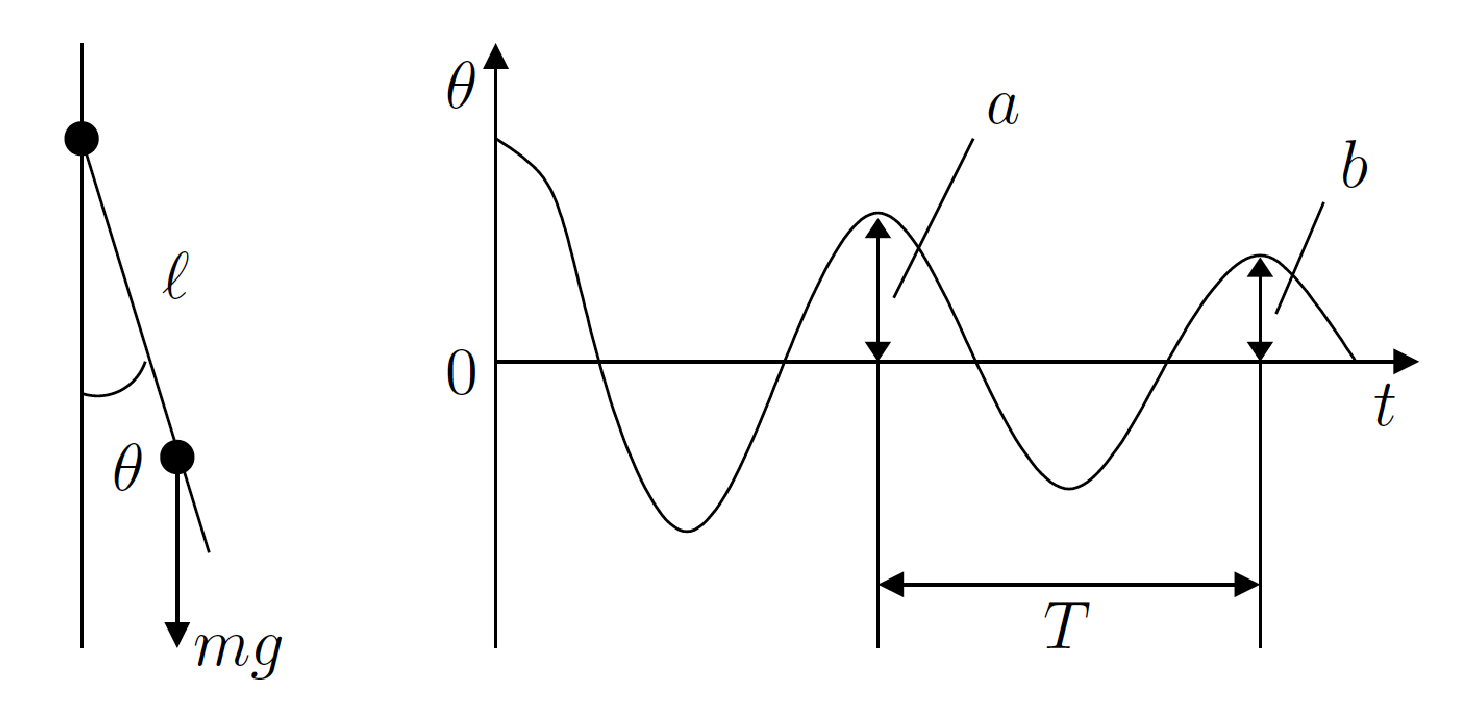
\includegraphics[width = 0.7 \linewidth]{measure_jc.eps}
		\caption{振子の自由振動}
		\label{fig:振子の自由振動}
=======
\begin{table}[hbtp]
	\begin{center}
=======
\begin{table}[hbtp]
	\begin{center}
>>>>>>> 1393f4f07a5b2b89c455e47e2d9b68edaf40a925
		\caption{物理パラメータ}
		\medskip
		\begin{tabular}{|ll|l|} \hline
			$m$ & $[\mathrm{kg}]$ & 0.038 \\ \hline
			$l$ & $[\mathrm{m}]$ & 0.12 \\ \hline
			$M(\rm{Step})$ & $[\mathrm{kg}]$ & 1.001 \\ \hline
			$f(\rm{Step})$ & $[\mathrm{kg/s}]$ & 9.67 \\ \hline
			$M(\rm{Feedback})$ & $[\mathrm{kg}]$ & 1.51 \\ \hline
			$f(\rm{Feedback})$ & $[\mathrm{kg/s}]$ & 16.5 \\ \hline
			$J$ & $[\mathrm{kgm^2}]$ & 3.9e-4 \\ \hline
			$c$ & $[\mathrm{kgm^2/s}]$ & 9.82e-5 \\ \hline
			$a$ & $[\mathrm{N/V}]$ & 0.49 \\ \hline
			$c_1$ & $[\mathrm{V/m}]$ & 1.0 \\ \hline
			$c_2$ & $[\mathrm{V/rad}]$ & 1.0 \\ \hline
			$g$ & $[\mathrm{m/s^2}]$ & 9.8 \\ \hline
		\end{tabular}
<<<<<<< HEAD
>>>>>>> c75b7fa605d82ac36c3c13370dbdcf9029f17b03
	\end{center}
\end{table}
=======
	\end{center}
\end{table}

	\subsection{$M$と$F$の検証}

	図\ref{fig:step11}、図\ref{fig:step12}、図\ref{fig:step13}、図\ref{fig:step14}、図\ref{fig:step15}は、それぞれ入力電圧11V,12V,13V,14V,15Vでのステップ応答により測定した$M$と$f$を用いたステップ制御のシミュレーションのデータと、実験のデータを重ね合わせたグラフである。シミュレーション結果と実験結果はほぼ一致しており、ステップ応答により求めたパラメータは適切であると考えられる。

	\begin{figure}[htbp]
		\begin{center}
			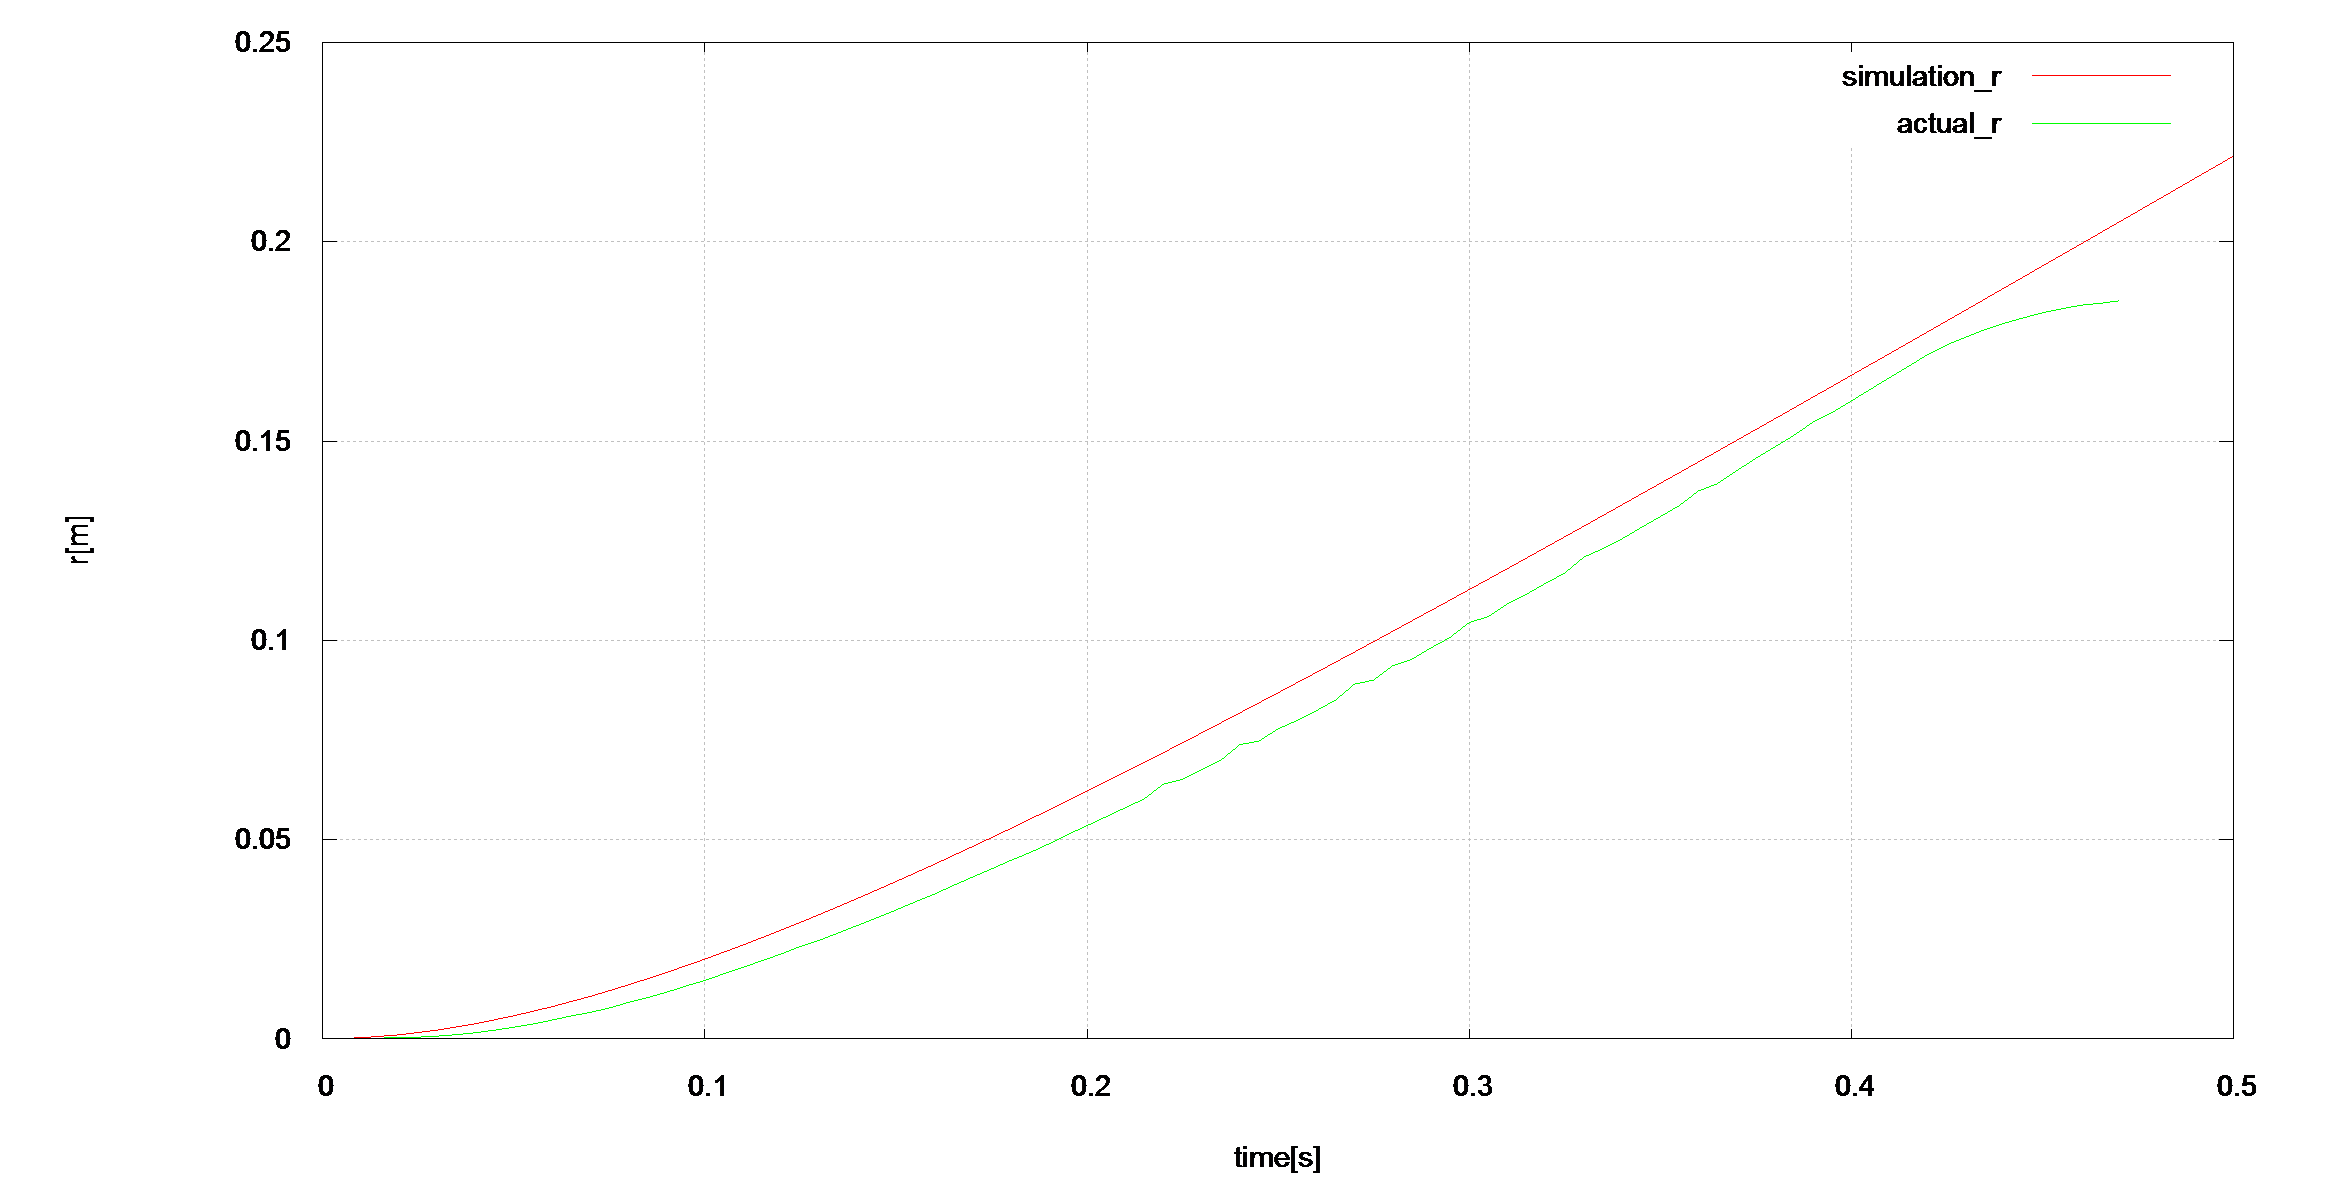
\includegraphics[width = 1.0 \linewidth]{step11.eps}
			\caption{入力電圧11VにおけるMとfの検証}
			\label{fig:step11}
		\end{center}
	\end{figure}

	\begin{figure}[htbp]
		\begin{center}
			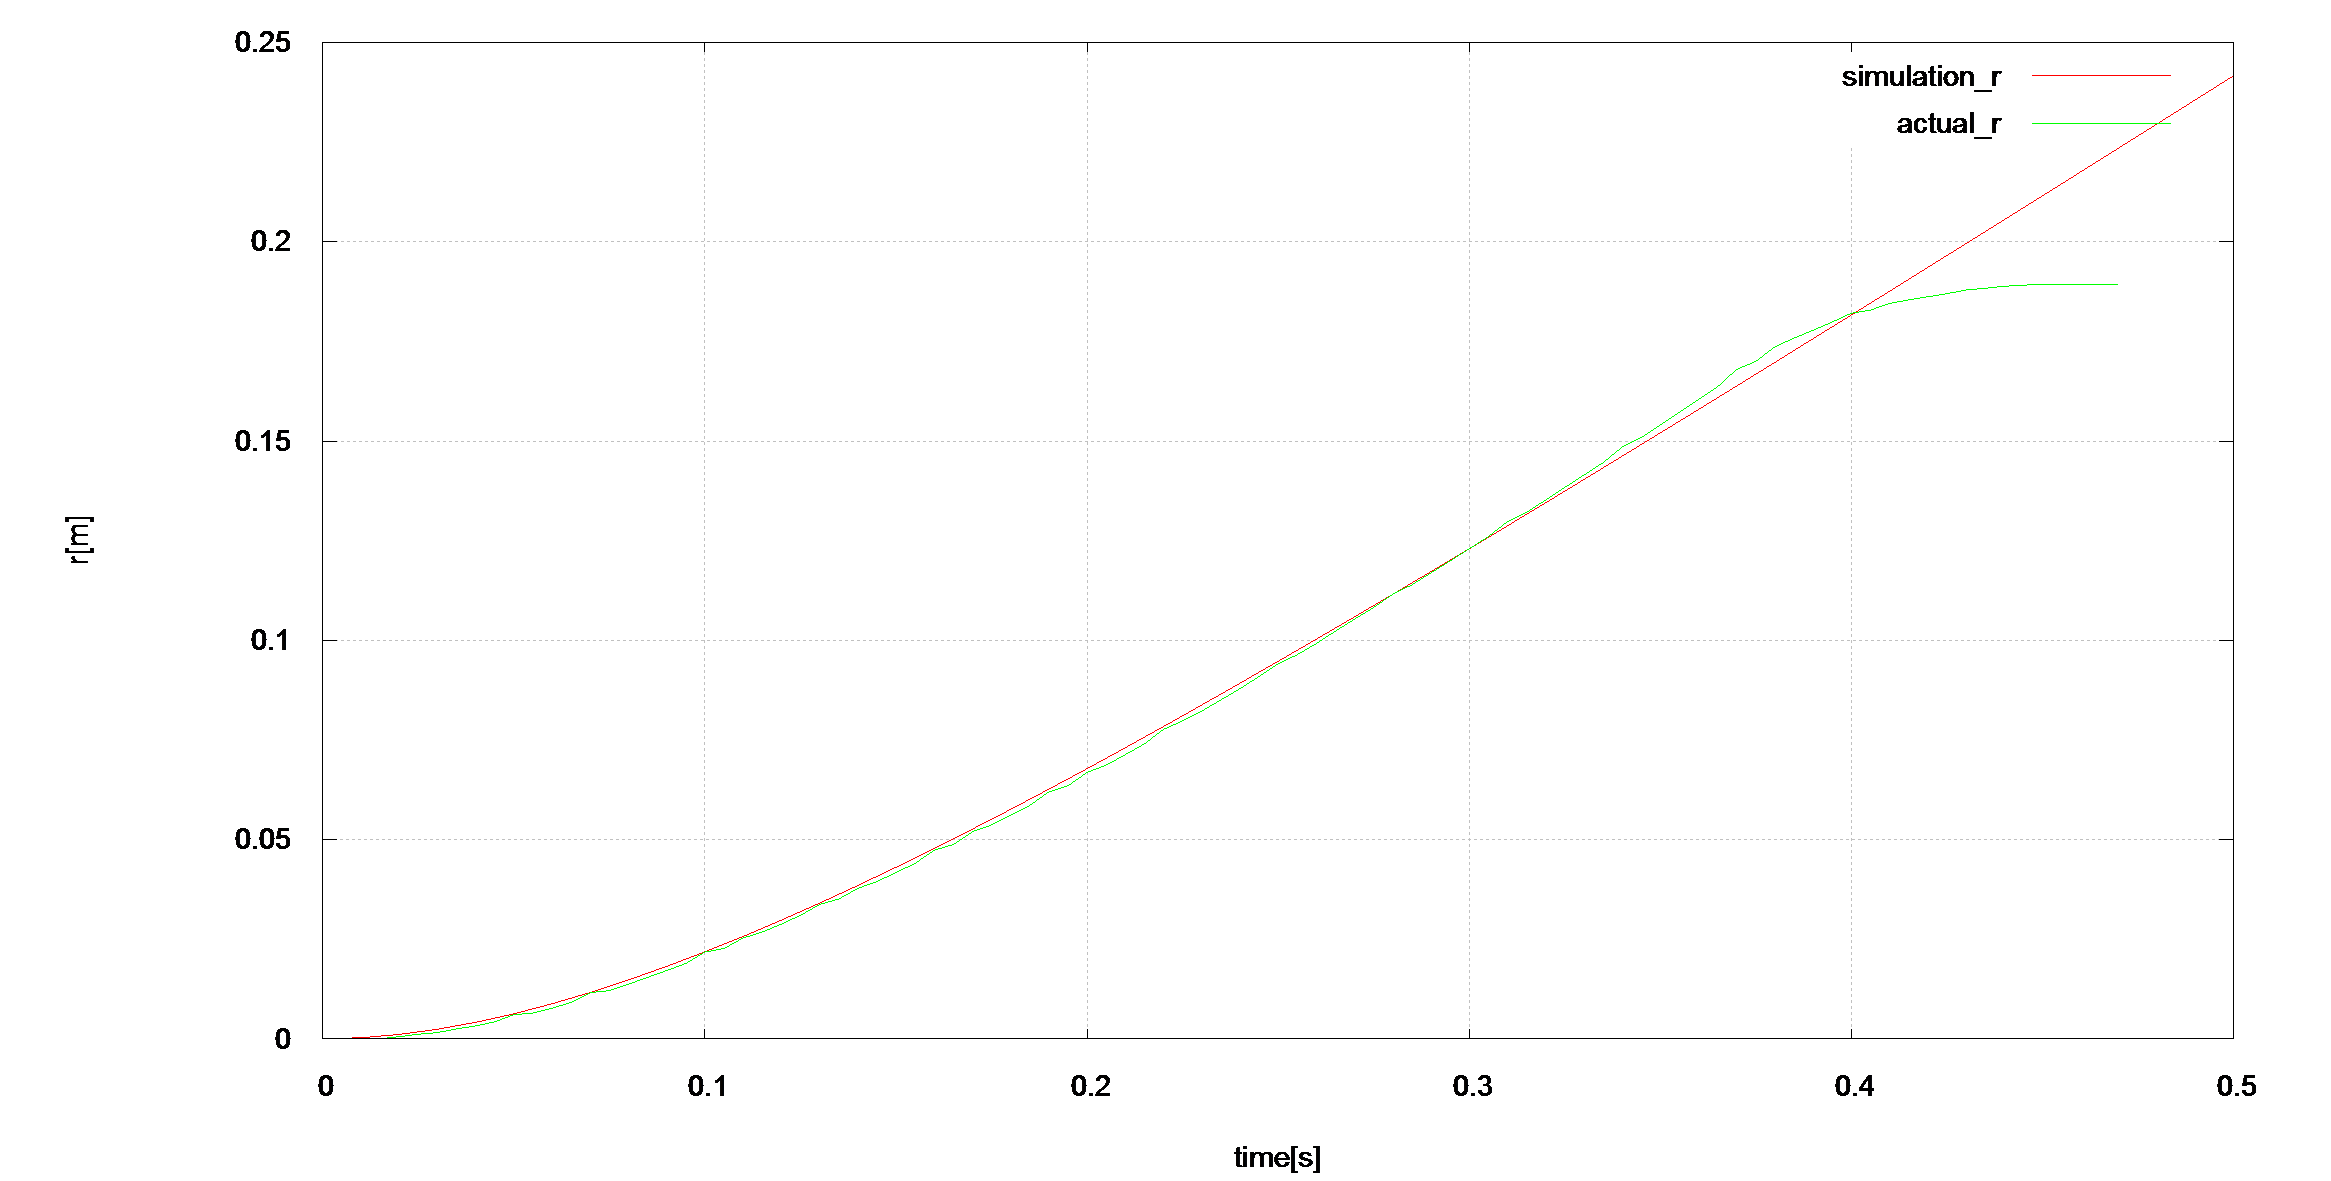
\includegraphics[width = 1.0 \linewidth]{step12.eps}
			\caption{入力電圧12VにおけるMとfの検証}
			\label{fig:step12}
		\end{center}
	\end{figure}
	
	\begin{figure}[htbp]
		\begin{center}
			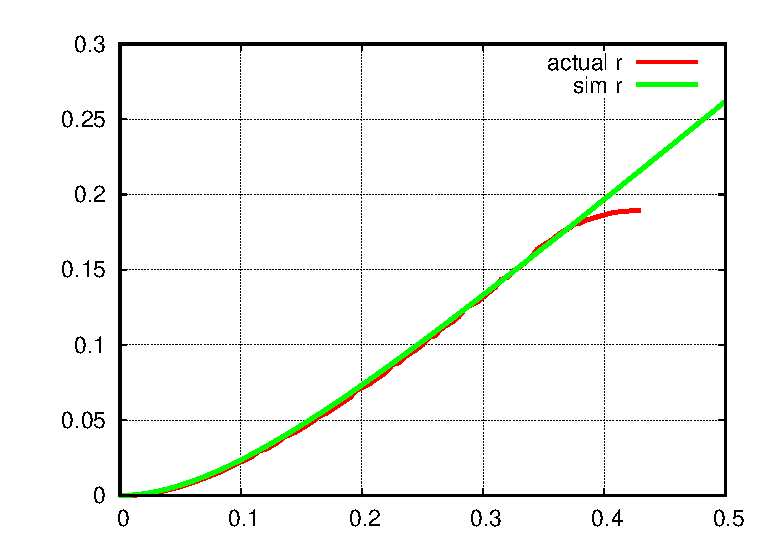
\includegraphics[width = 1.0 \linewidth]{step13.eps}
			\caption{入力電圧13VにおけるMとfの検証}
			\label{fig:step13}
		\end{center}
	\end{figure}
	
	\begin{figure}[htbp]
		\begin{center}
			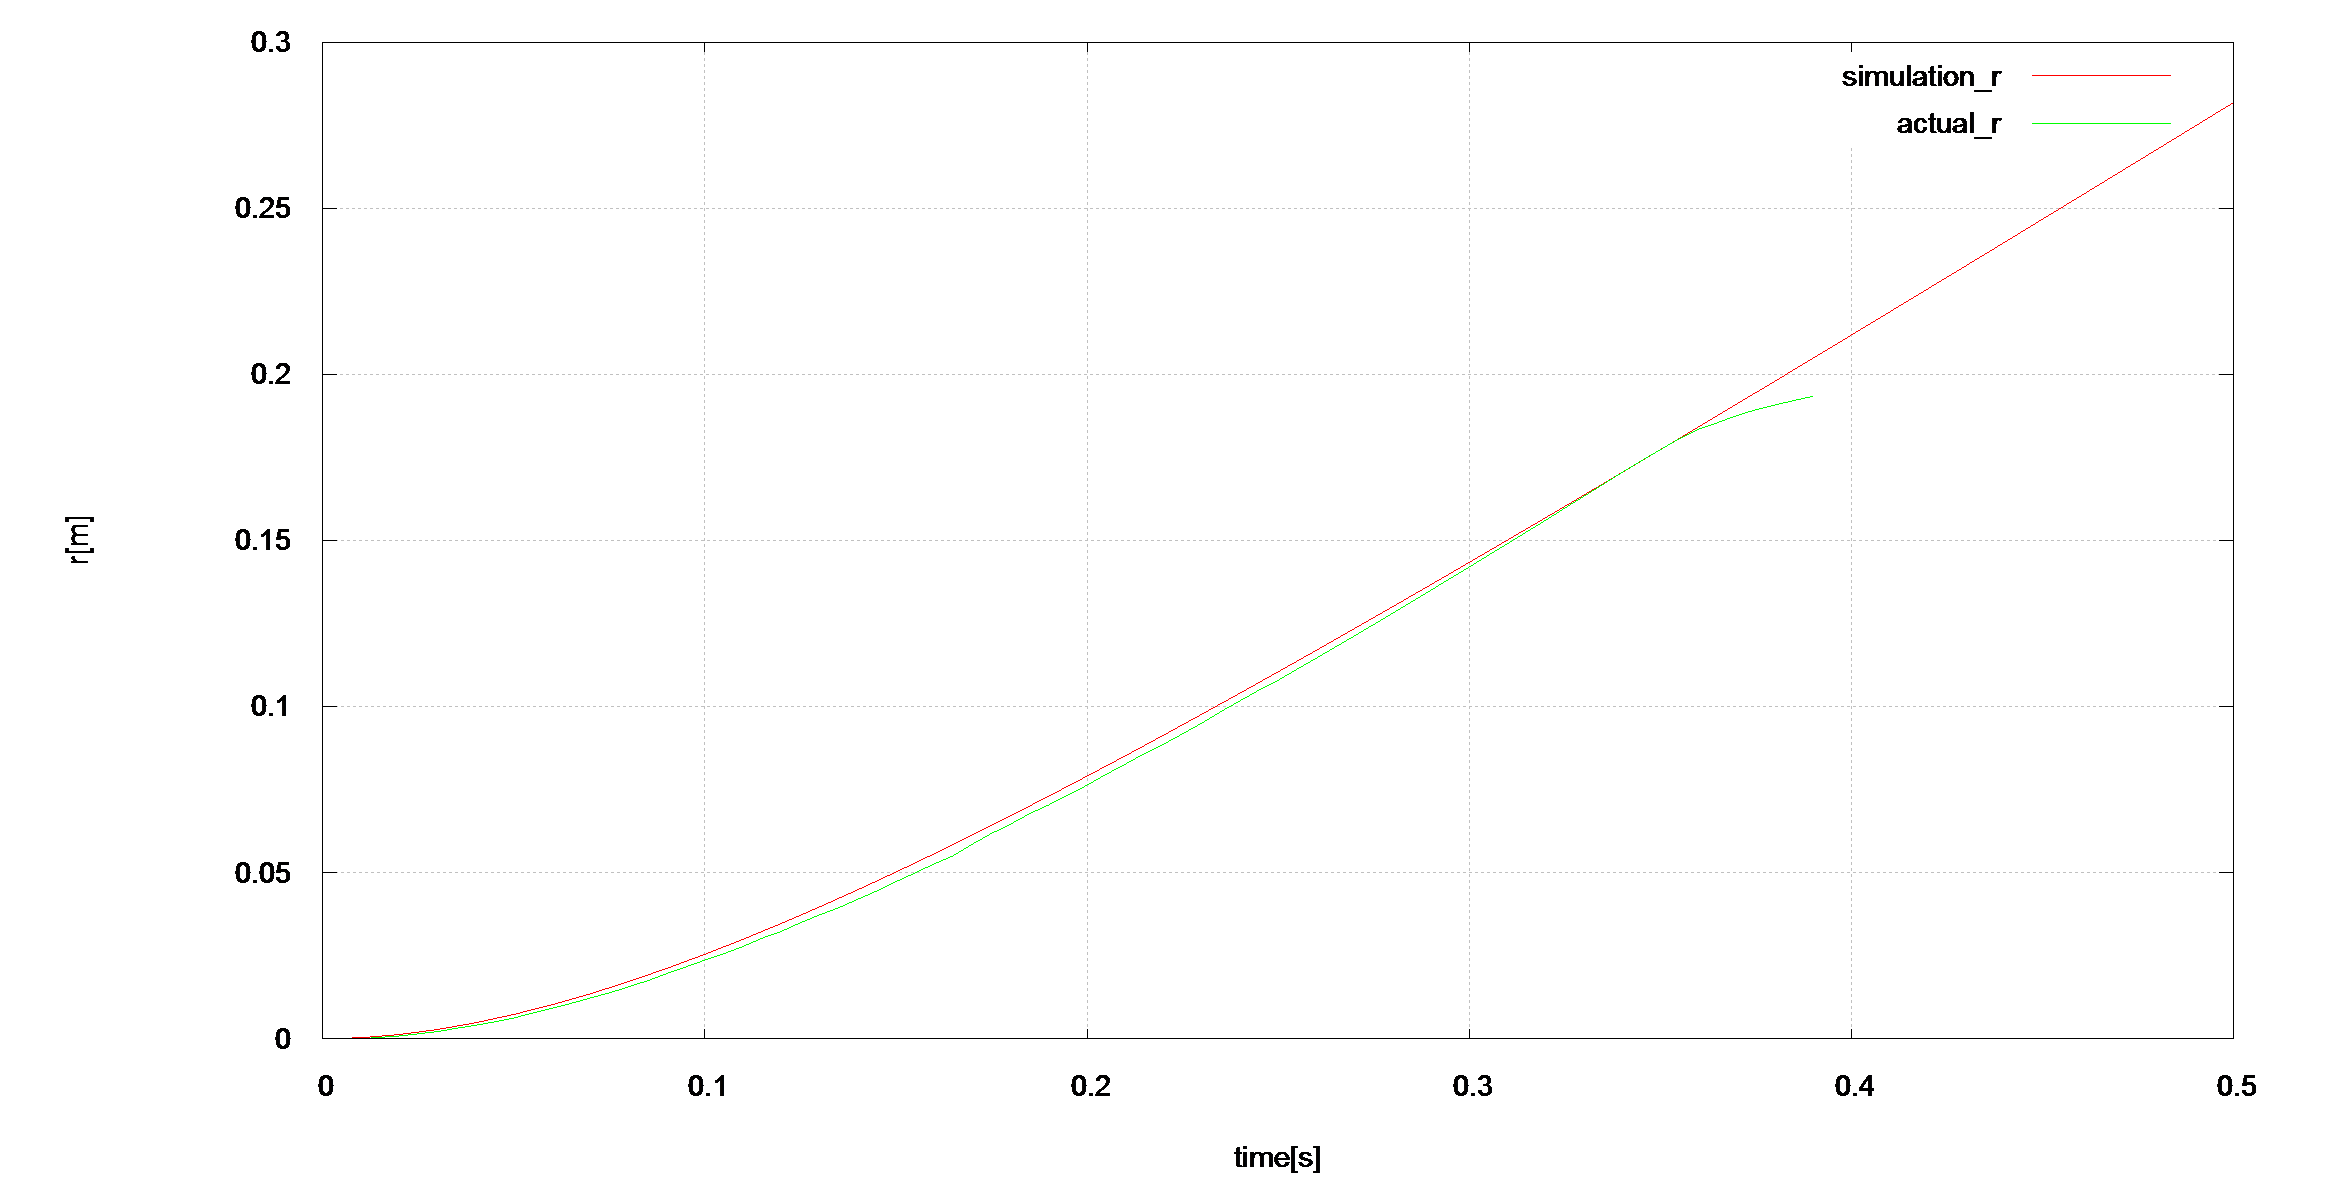
\includegraphics[width = 1.0 \linewidth]{step14.eps}
			\caption{入力電圧14VにおけるMとfの検証}
			\label{fig:step14}
		\end{center}
	\end{figure}
	
	\begin{figure}[htbp]
		\begin{center}
			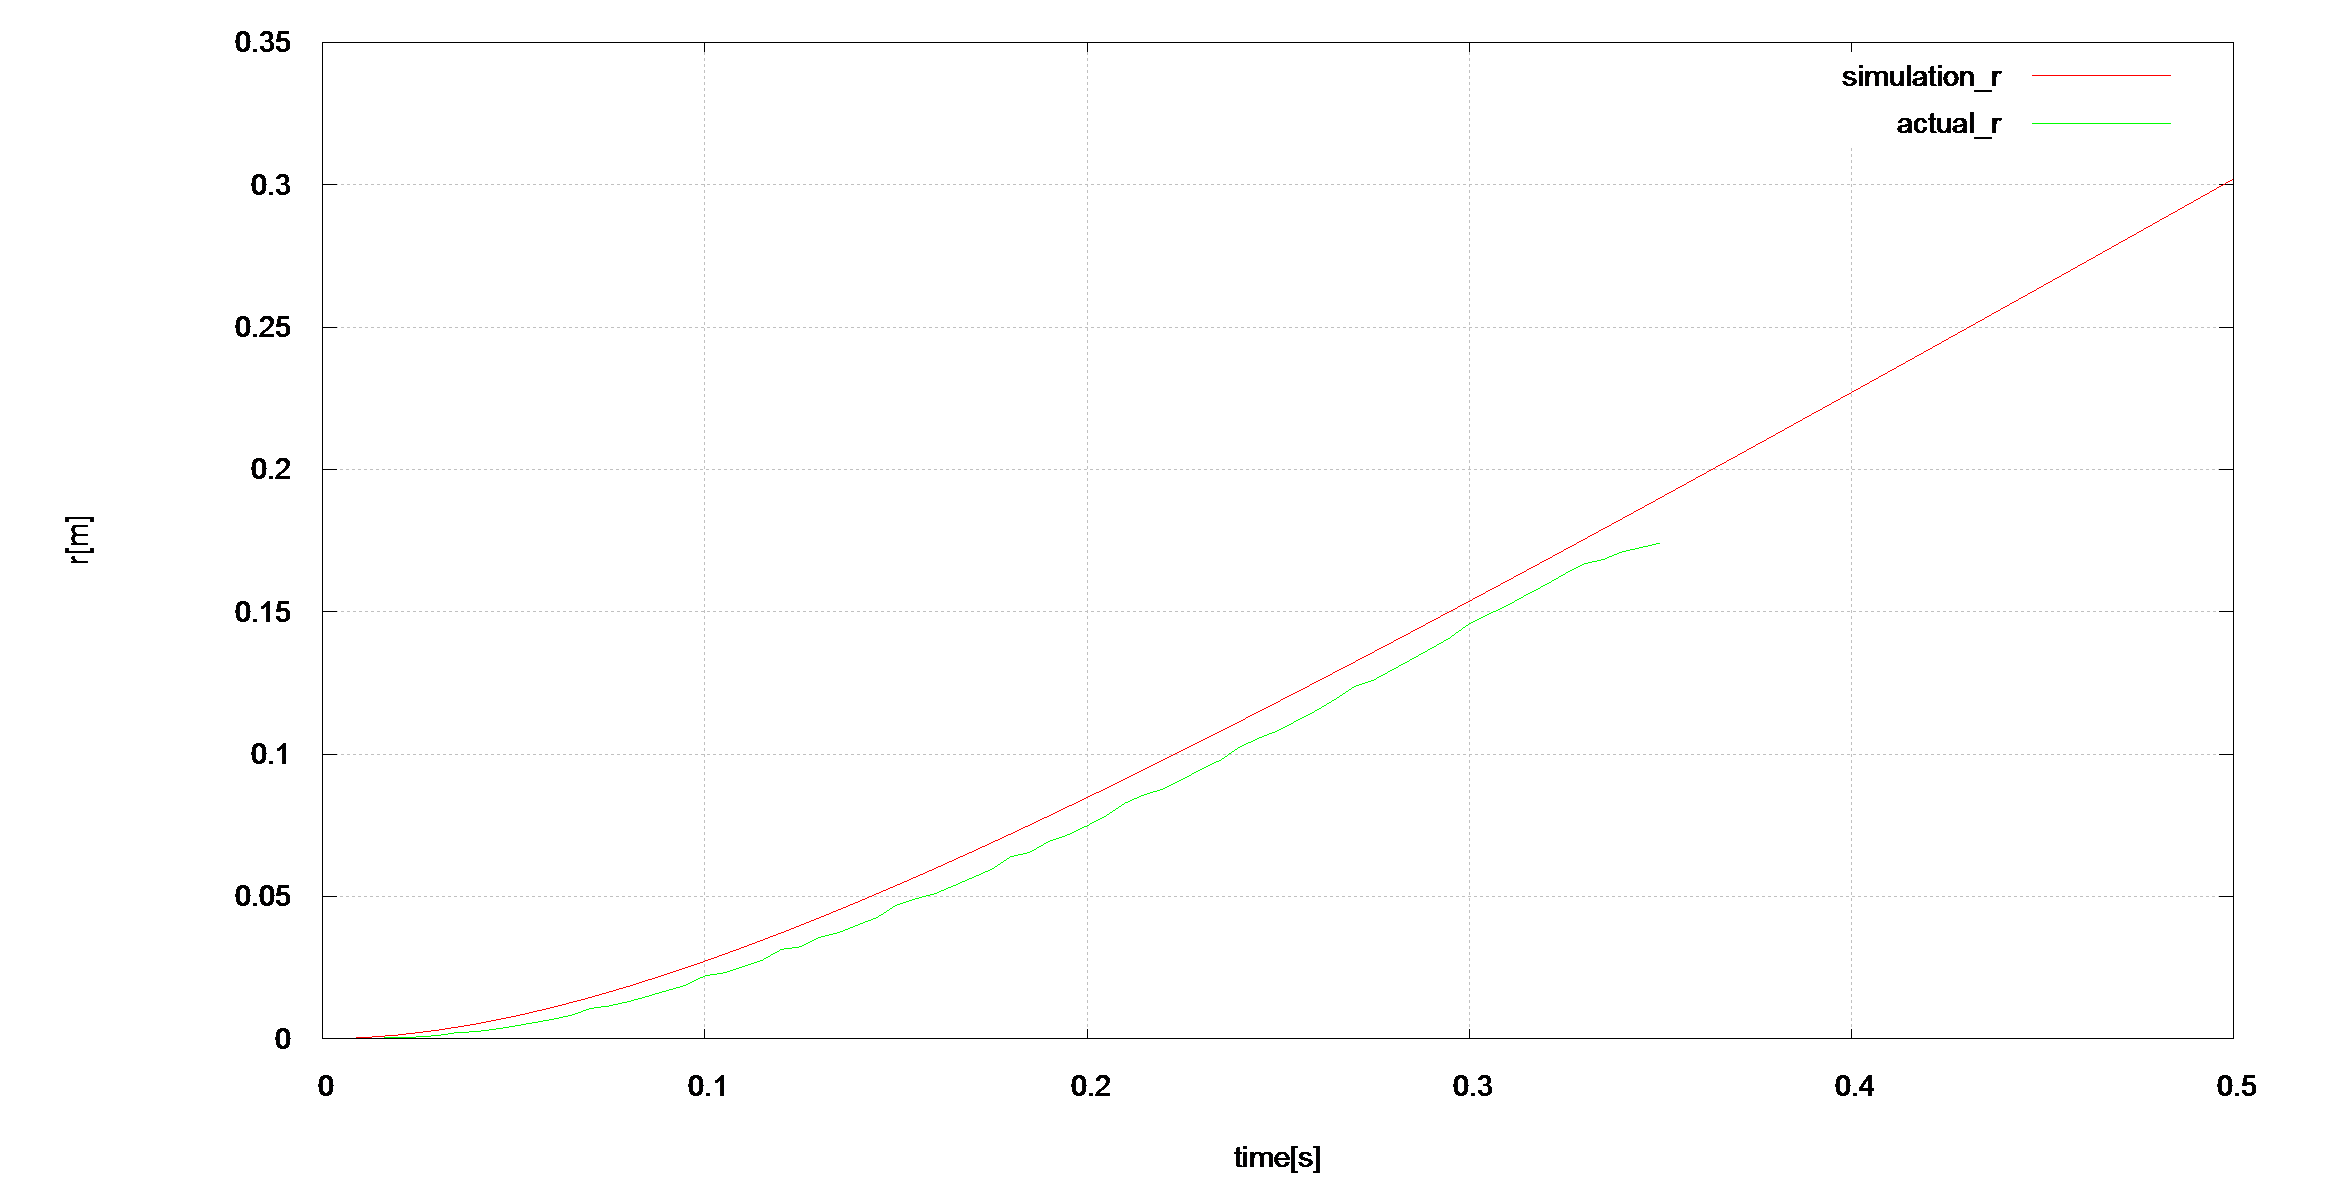
\includegraphics[width = 1.0 \linewidth]{step15.eps}
			\caption{入力電圧15VにおけるMとfの検証}
			\label{fig:step15}
		\end{center}
	\end{figure}
	
	
	\subsection{$J$と$c$の検証}
	\begin{figure}[htbp]
		\begin{center}
			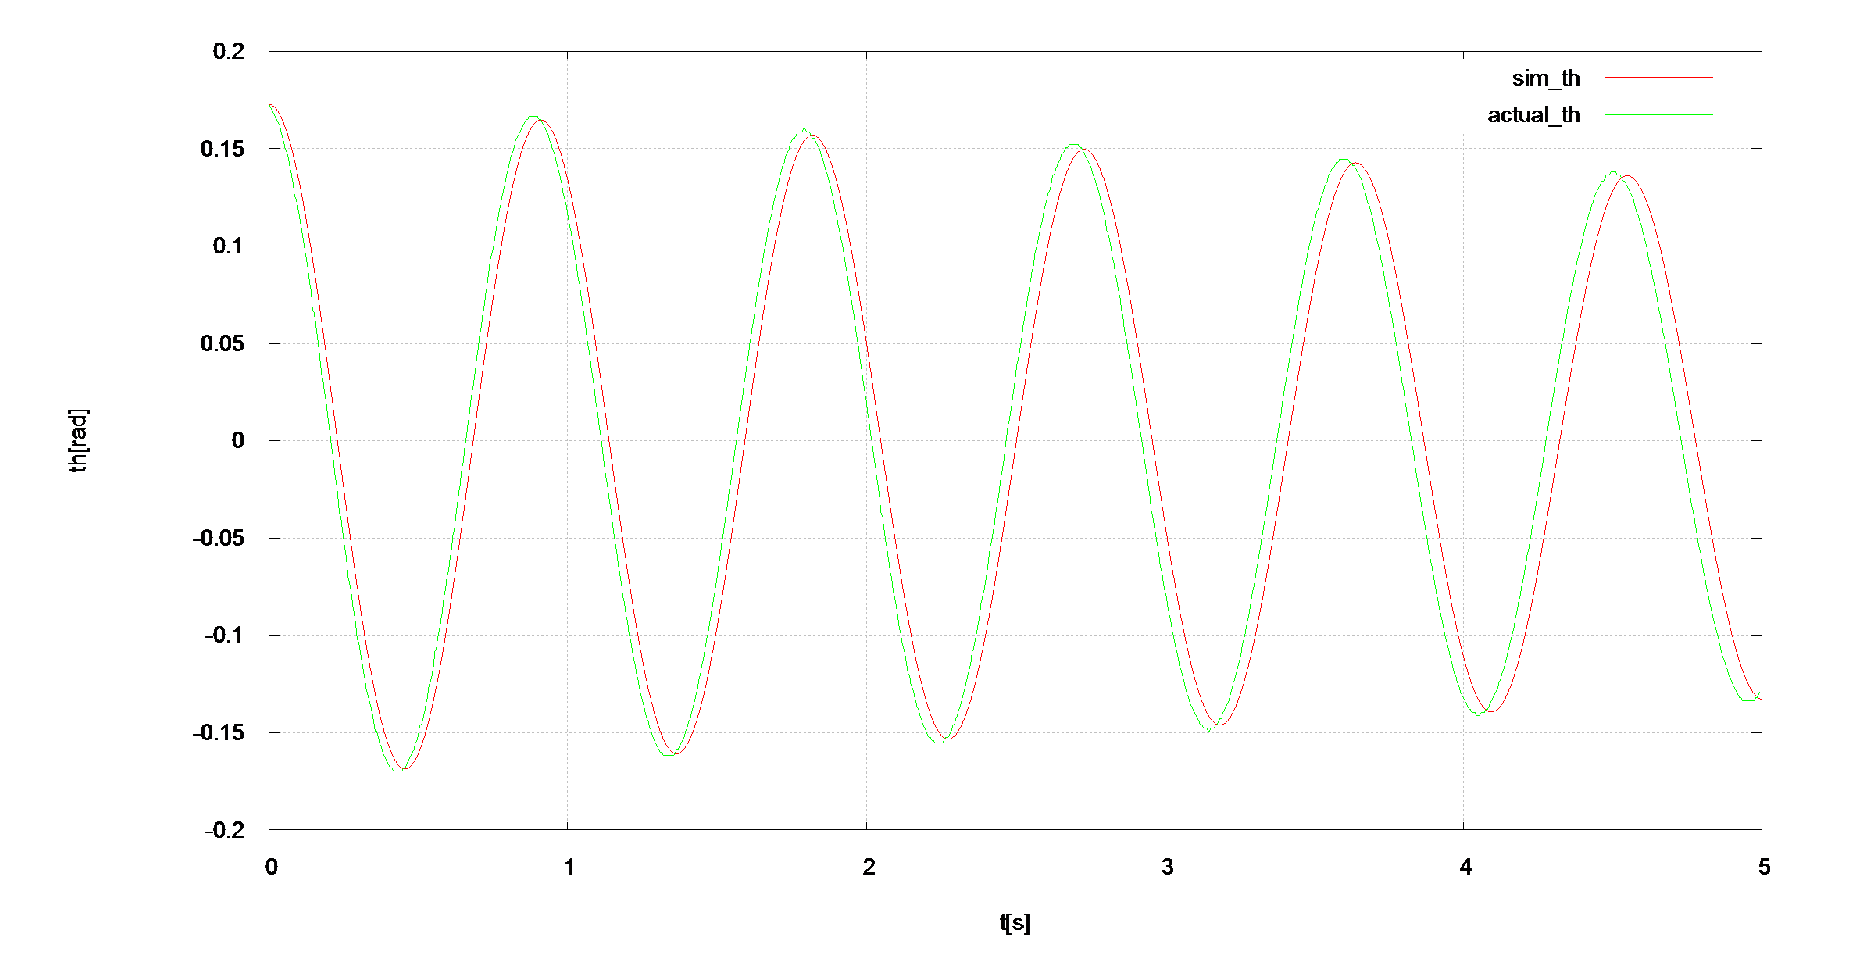
\includegraphics[width = 1.0 \linewidth]{freePendulum.eps}
			\caption{測定した$J$と$c$を用いたシミュレーションと実験データ}
			\label{fig:Jc}
		\end{center}
	\end{figure}
	図\ref{fig:Jc}、は測定した$J$と$c$を用いた自由振動のシミュレーションのデータと、
	実際の自由振動の実験結果を重ね合わせたグラフである。
>>>>>>> 1393f4f07a5b2b89c455e47e2d9b68edaf40a925

	\subsection{$M$と$F$の検証}

<<<<<<< HEAD
	図\ref{fig:step11}、図\ref{fig:step12}、図\ref{fig:step13}、図\ref{fig:step14}、図\ref{fig:step15}は、それぞれ入力電圧11V,12V,13V,14V,15Vでのステップ応答により測定した$M$と$f$を用いたステップ制御のシミュレーションのデータと、実験のデータを重ね合わせたグラフである。シミュレーション結果と実験結果はほぼ一致しており、ステップ応答により求めたパラメータは適切であると考えられる。
 \clearpage
	\begin{figure}[htbp]
		\begin{center}
			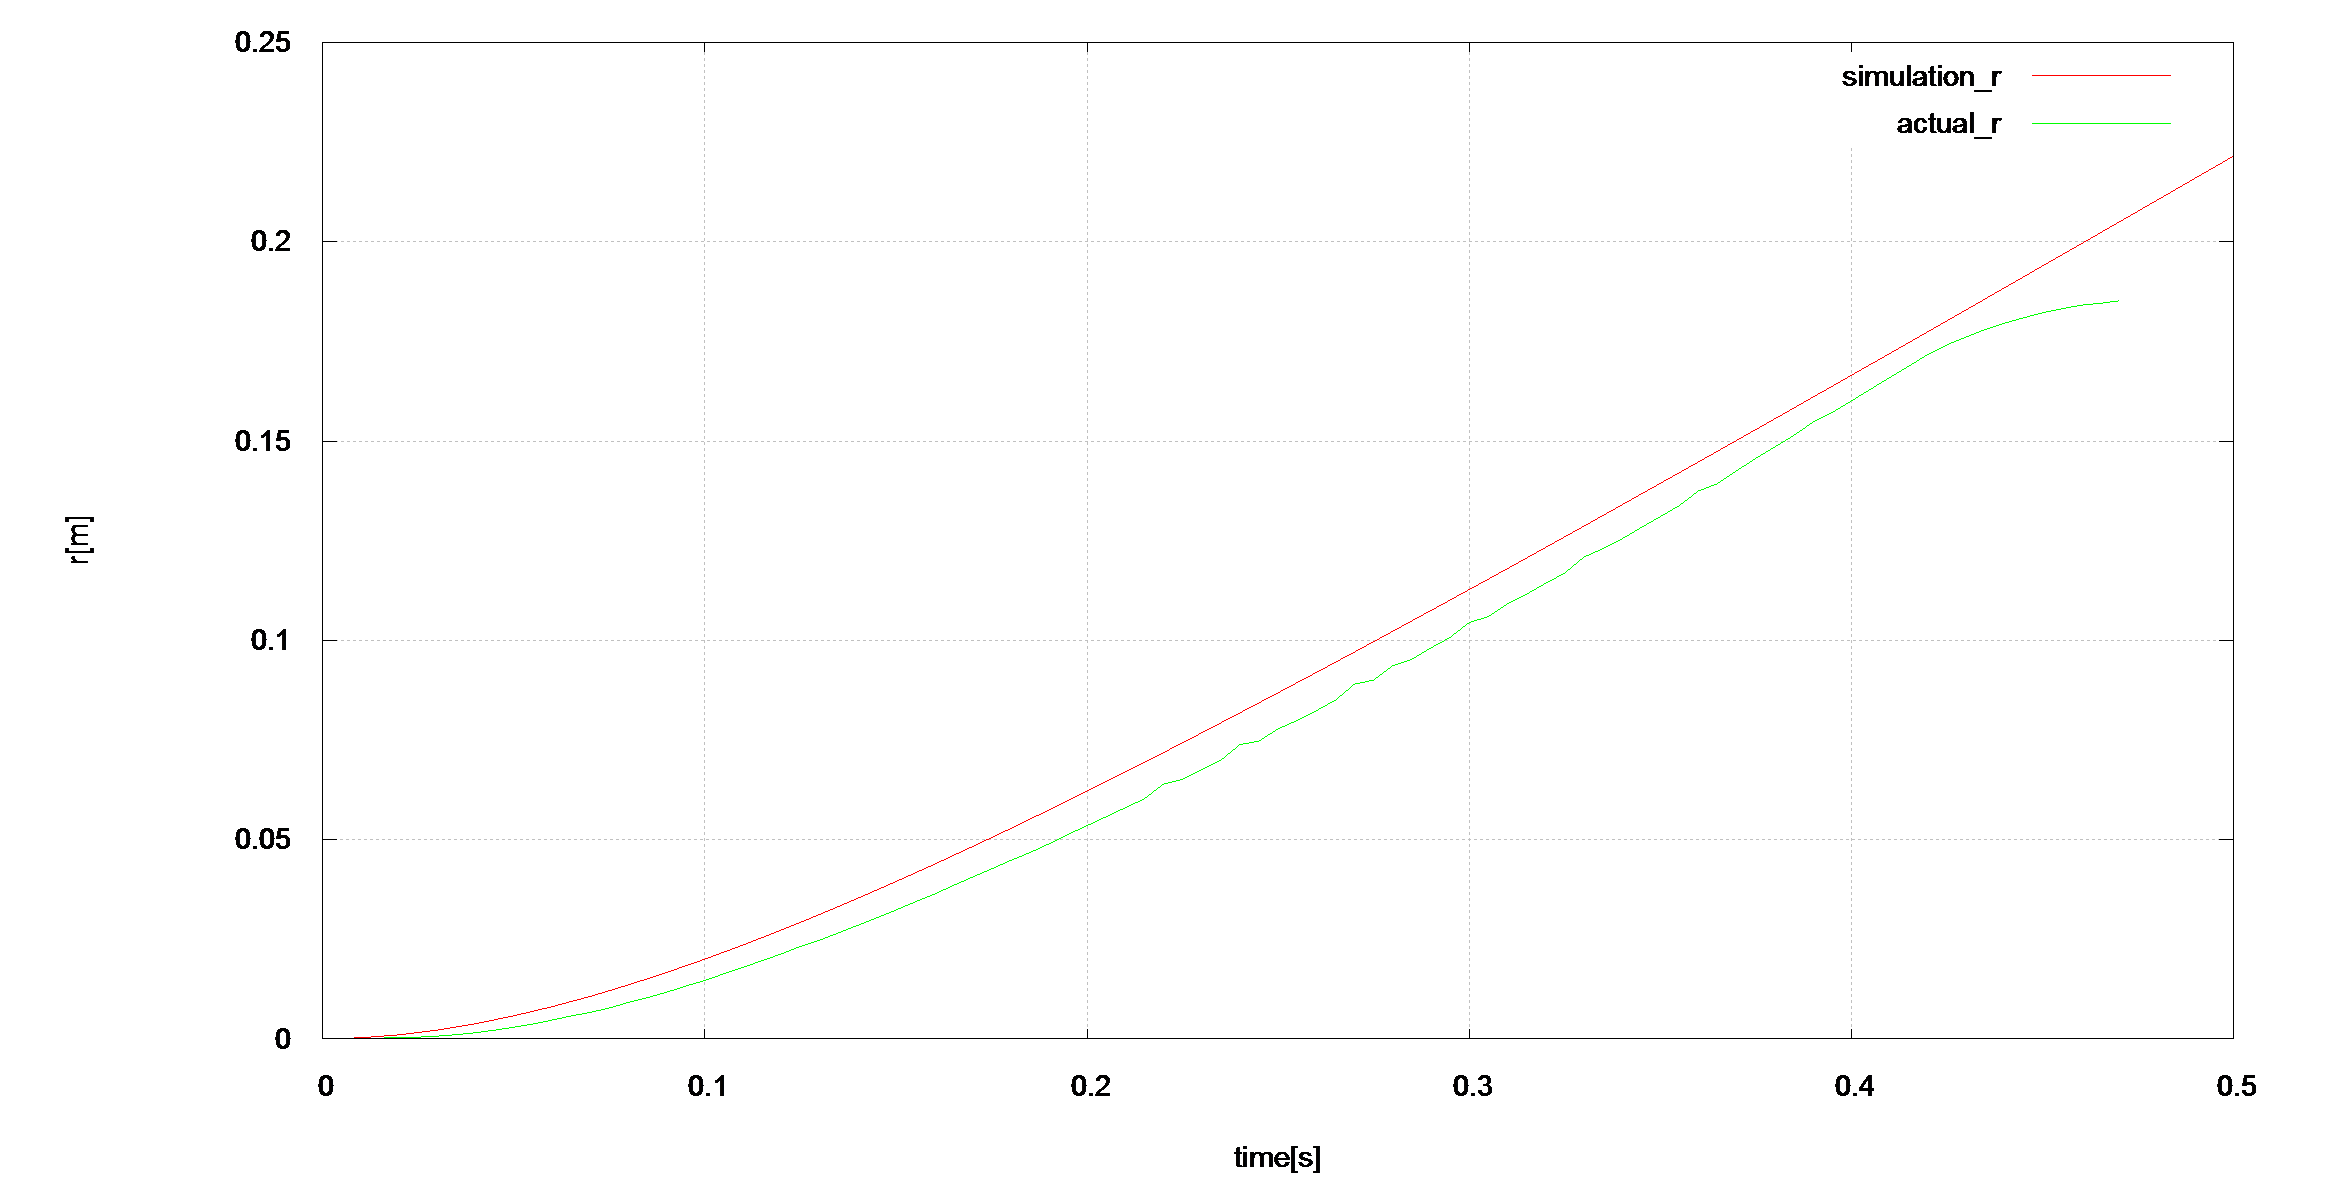
\includegraphics[width = 1.0 \linewidth]{step11.eps}
			\caption{入力電圧11VにおけるMとfの検証}
			\label{fig:step11}
		\end{center}
	\end{figure}

	\begin{figure}[htbp]
		\begin{center}
			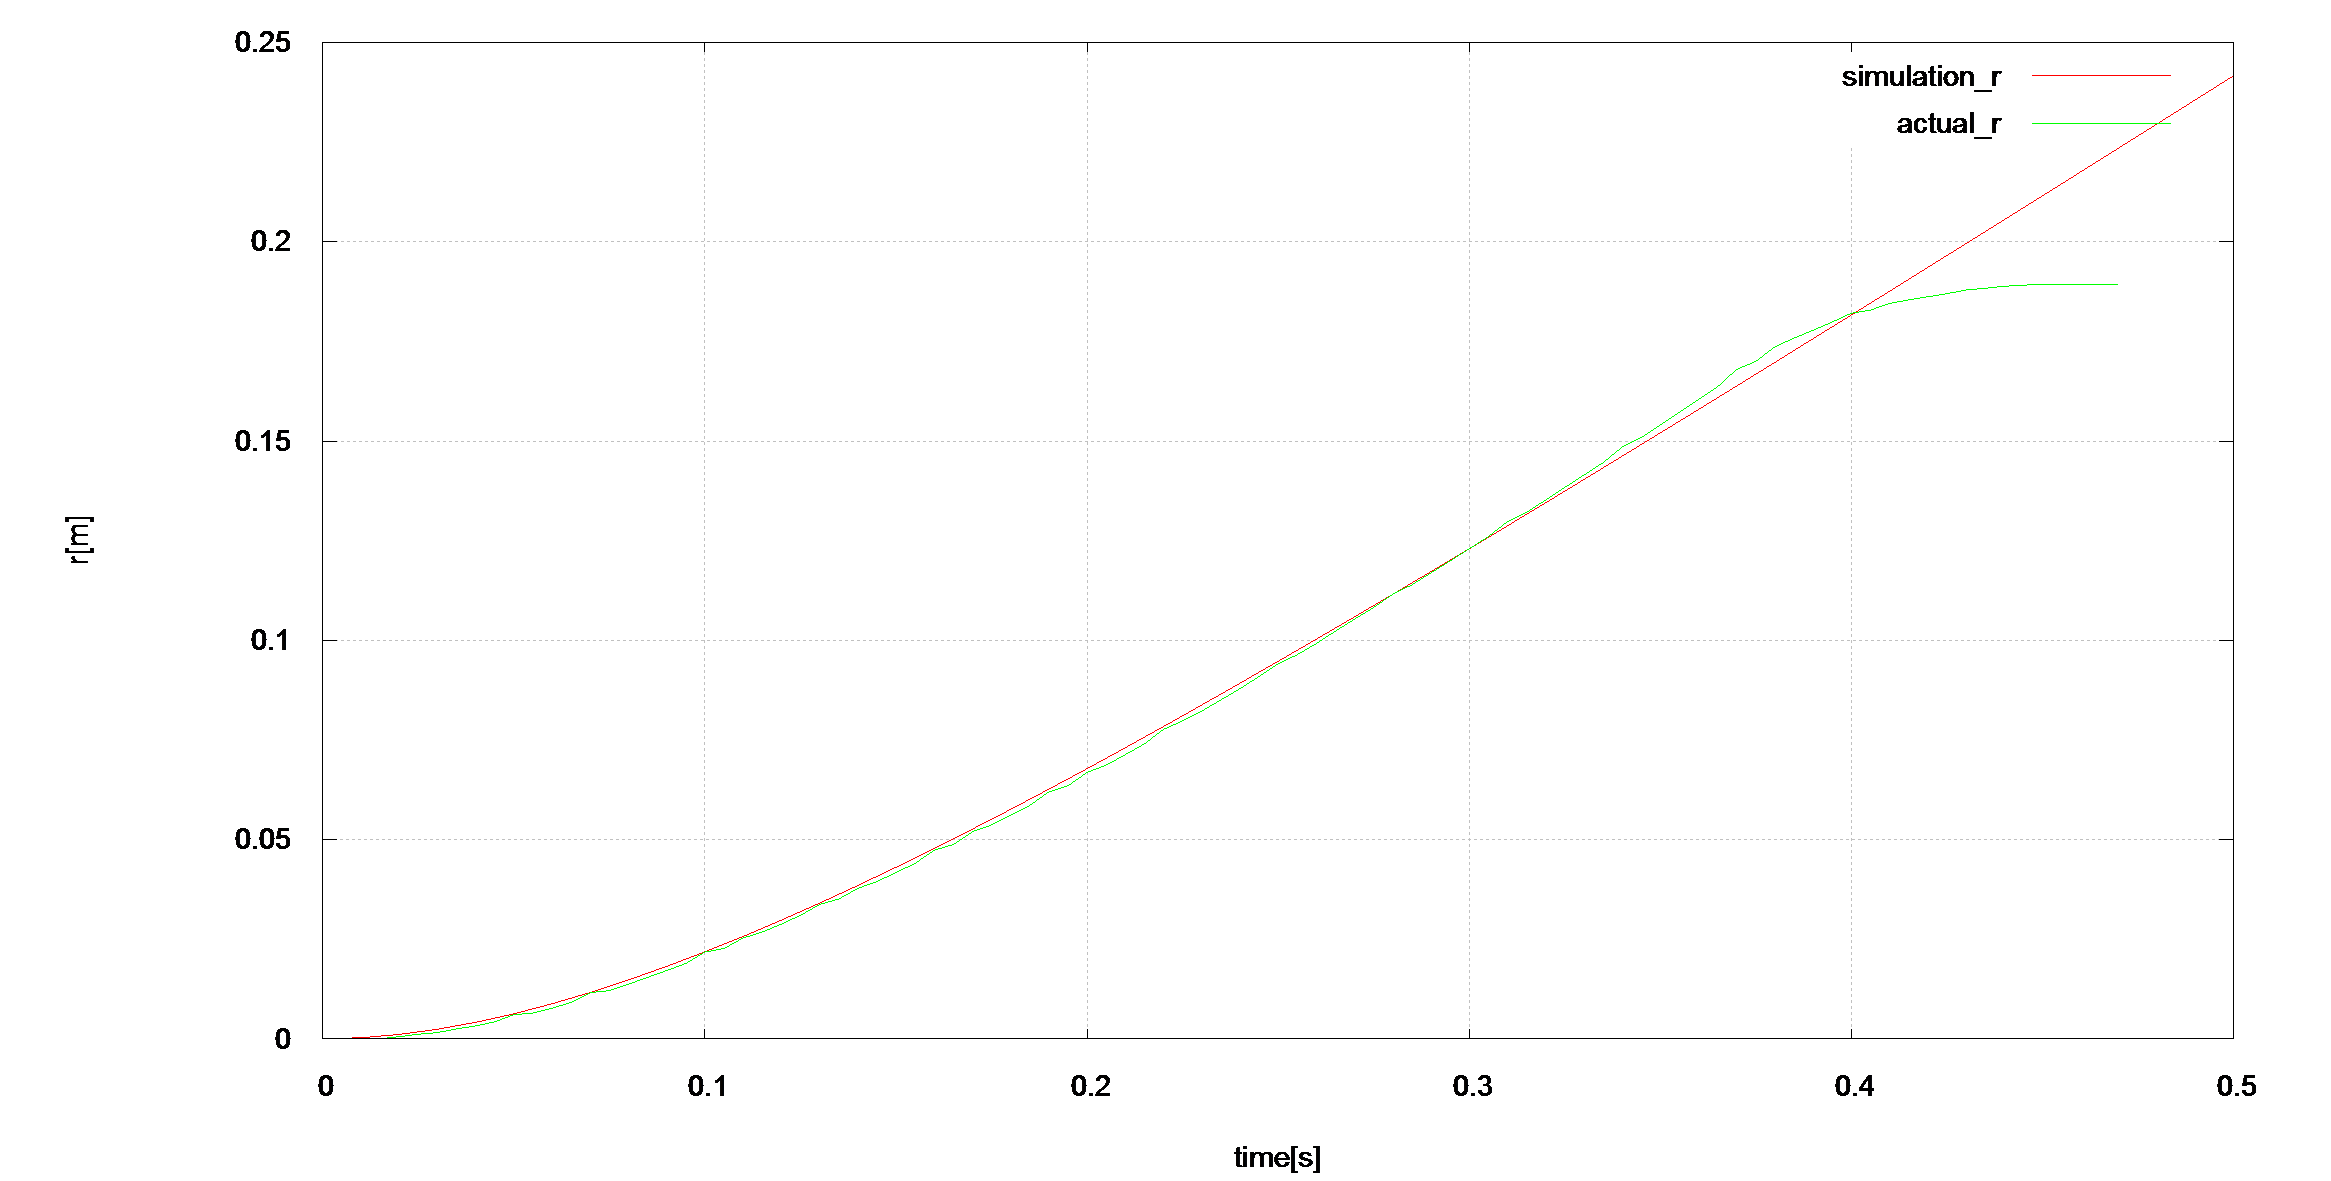
\includegraphics[width = 1.0 \linewidth]{step12.eps}
			\caption{入力電圧12VにおけるMとfの検証}
			\label{fig:step12}
		\end{center}
	\end{figure}
	
	\begin{figure}[htbp]
		\begin{center}
			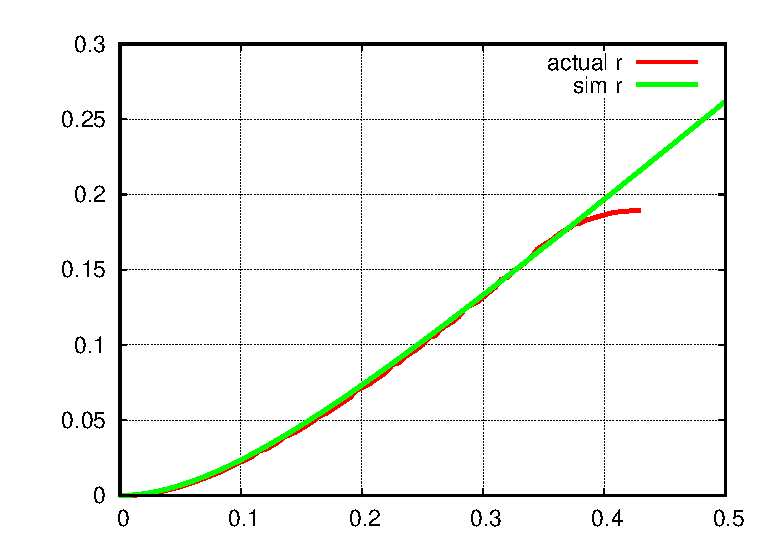
\includegraphics[width = 1.0 \linewidth]{step13.eps}
			\caption{入力電圧13VにおけるMとfの検証}
			\label{fig:step13}
		\end{center}
	\end{figure}
	
	\begin{figure}[htbp]
		\begin{center}
			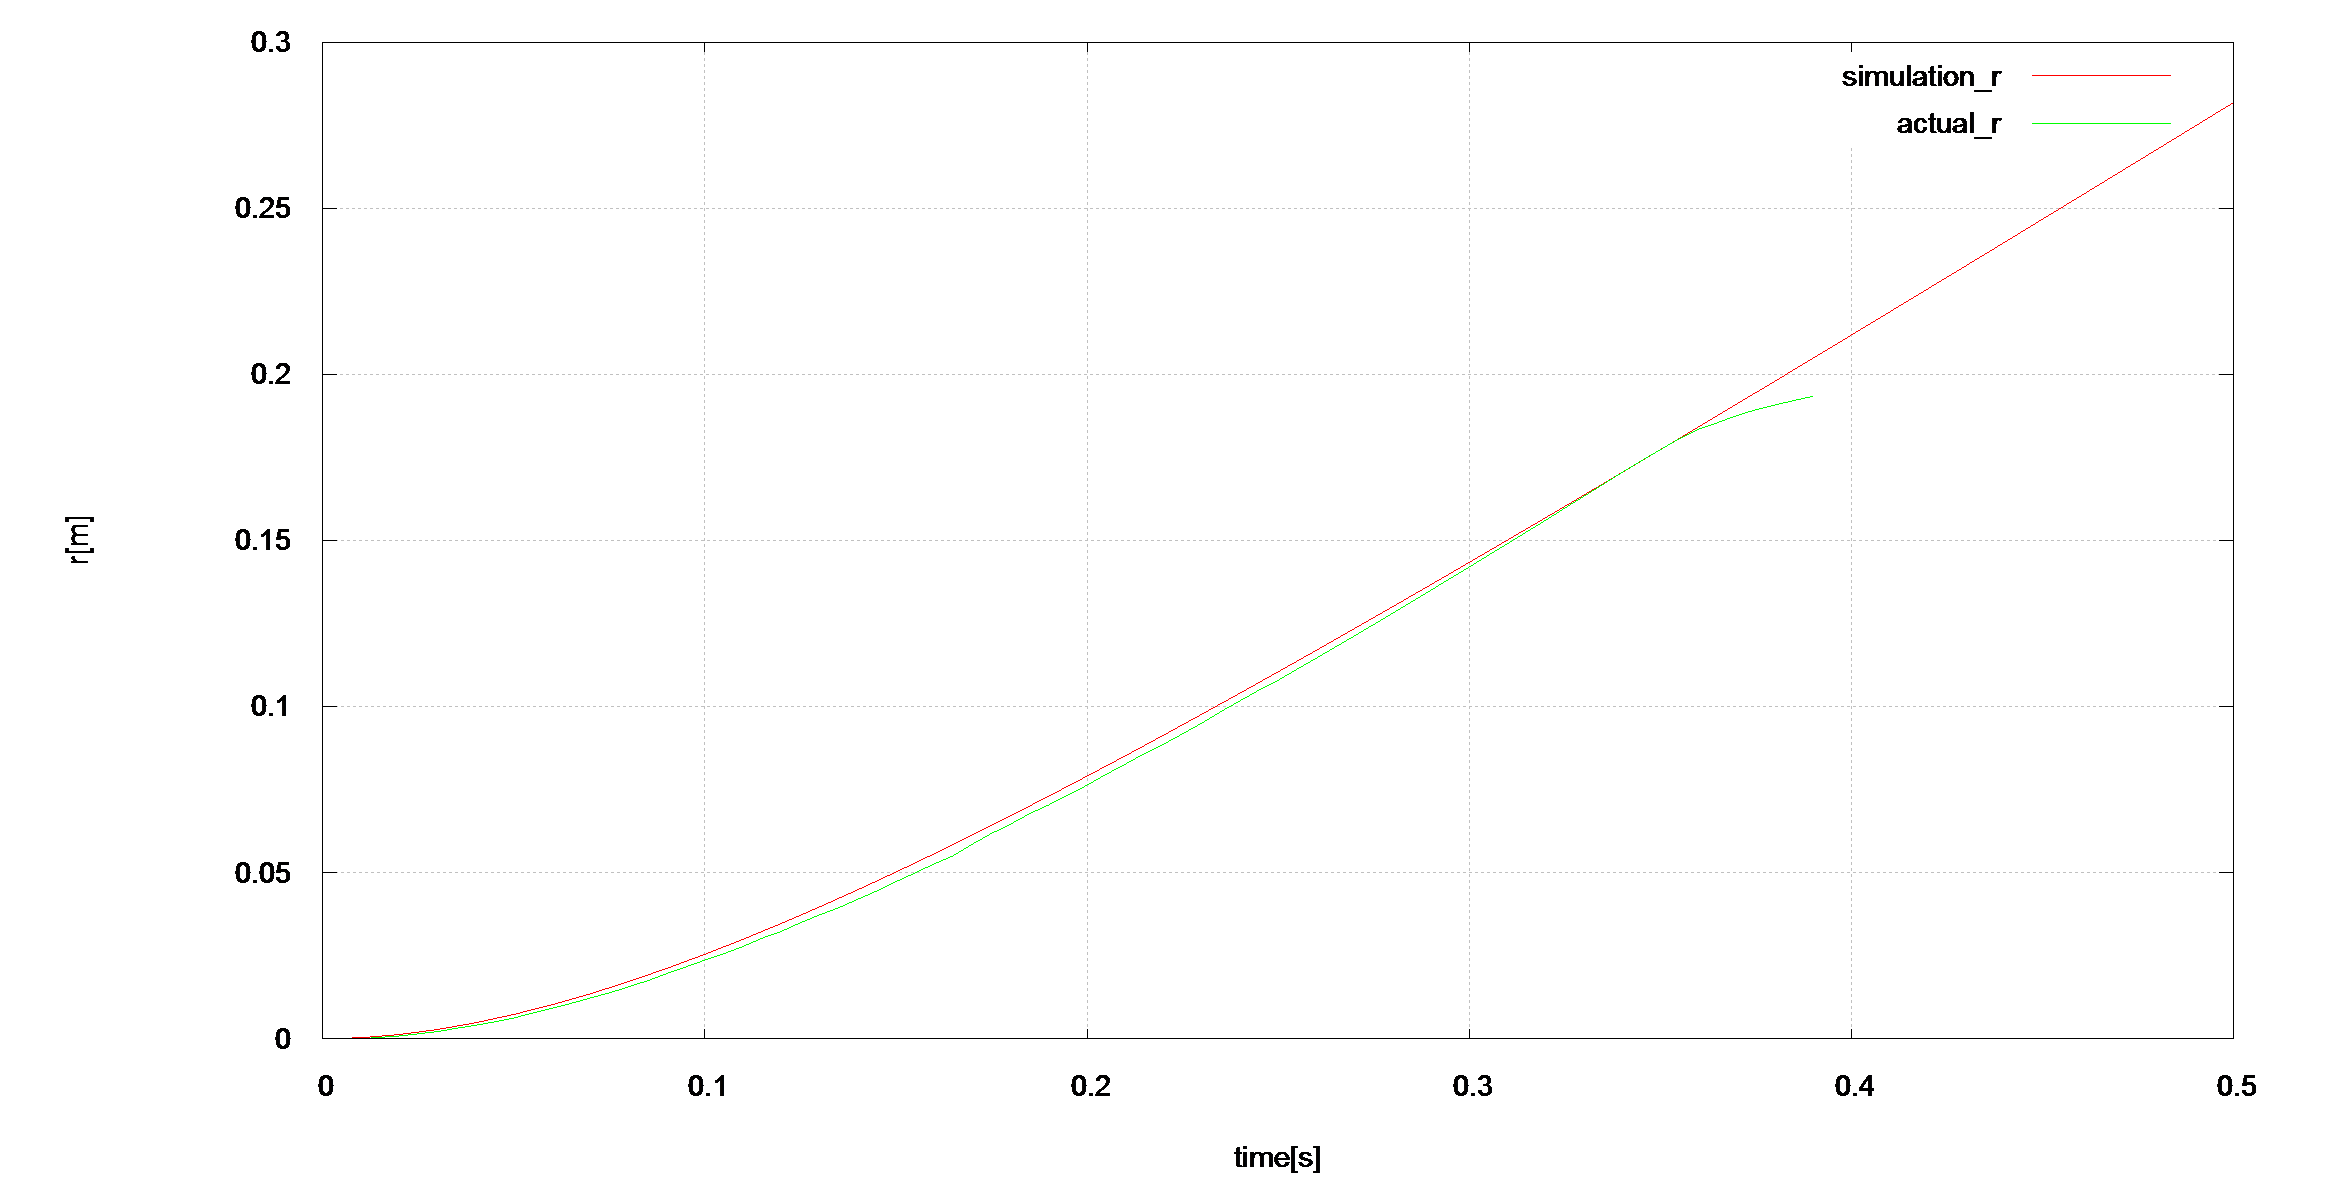
\includegraphics[width = 1.0 \linewidth]{step14.eps}
			\caption{入力電圧14VにおけるMとfの検証}
			\label{fig:step14}
		\end{center}
	\end{figure}
	
	\begin{figure}[htbp]
		\begin{center}
			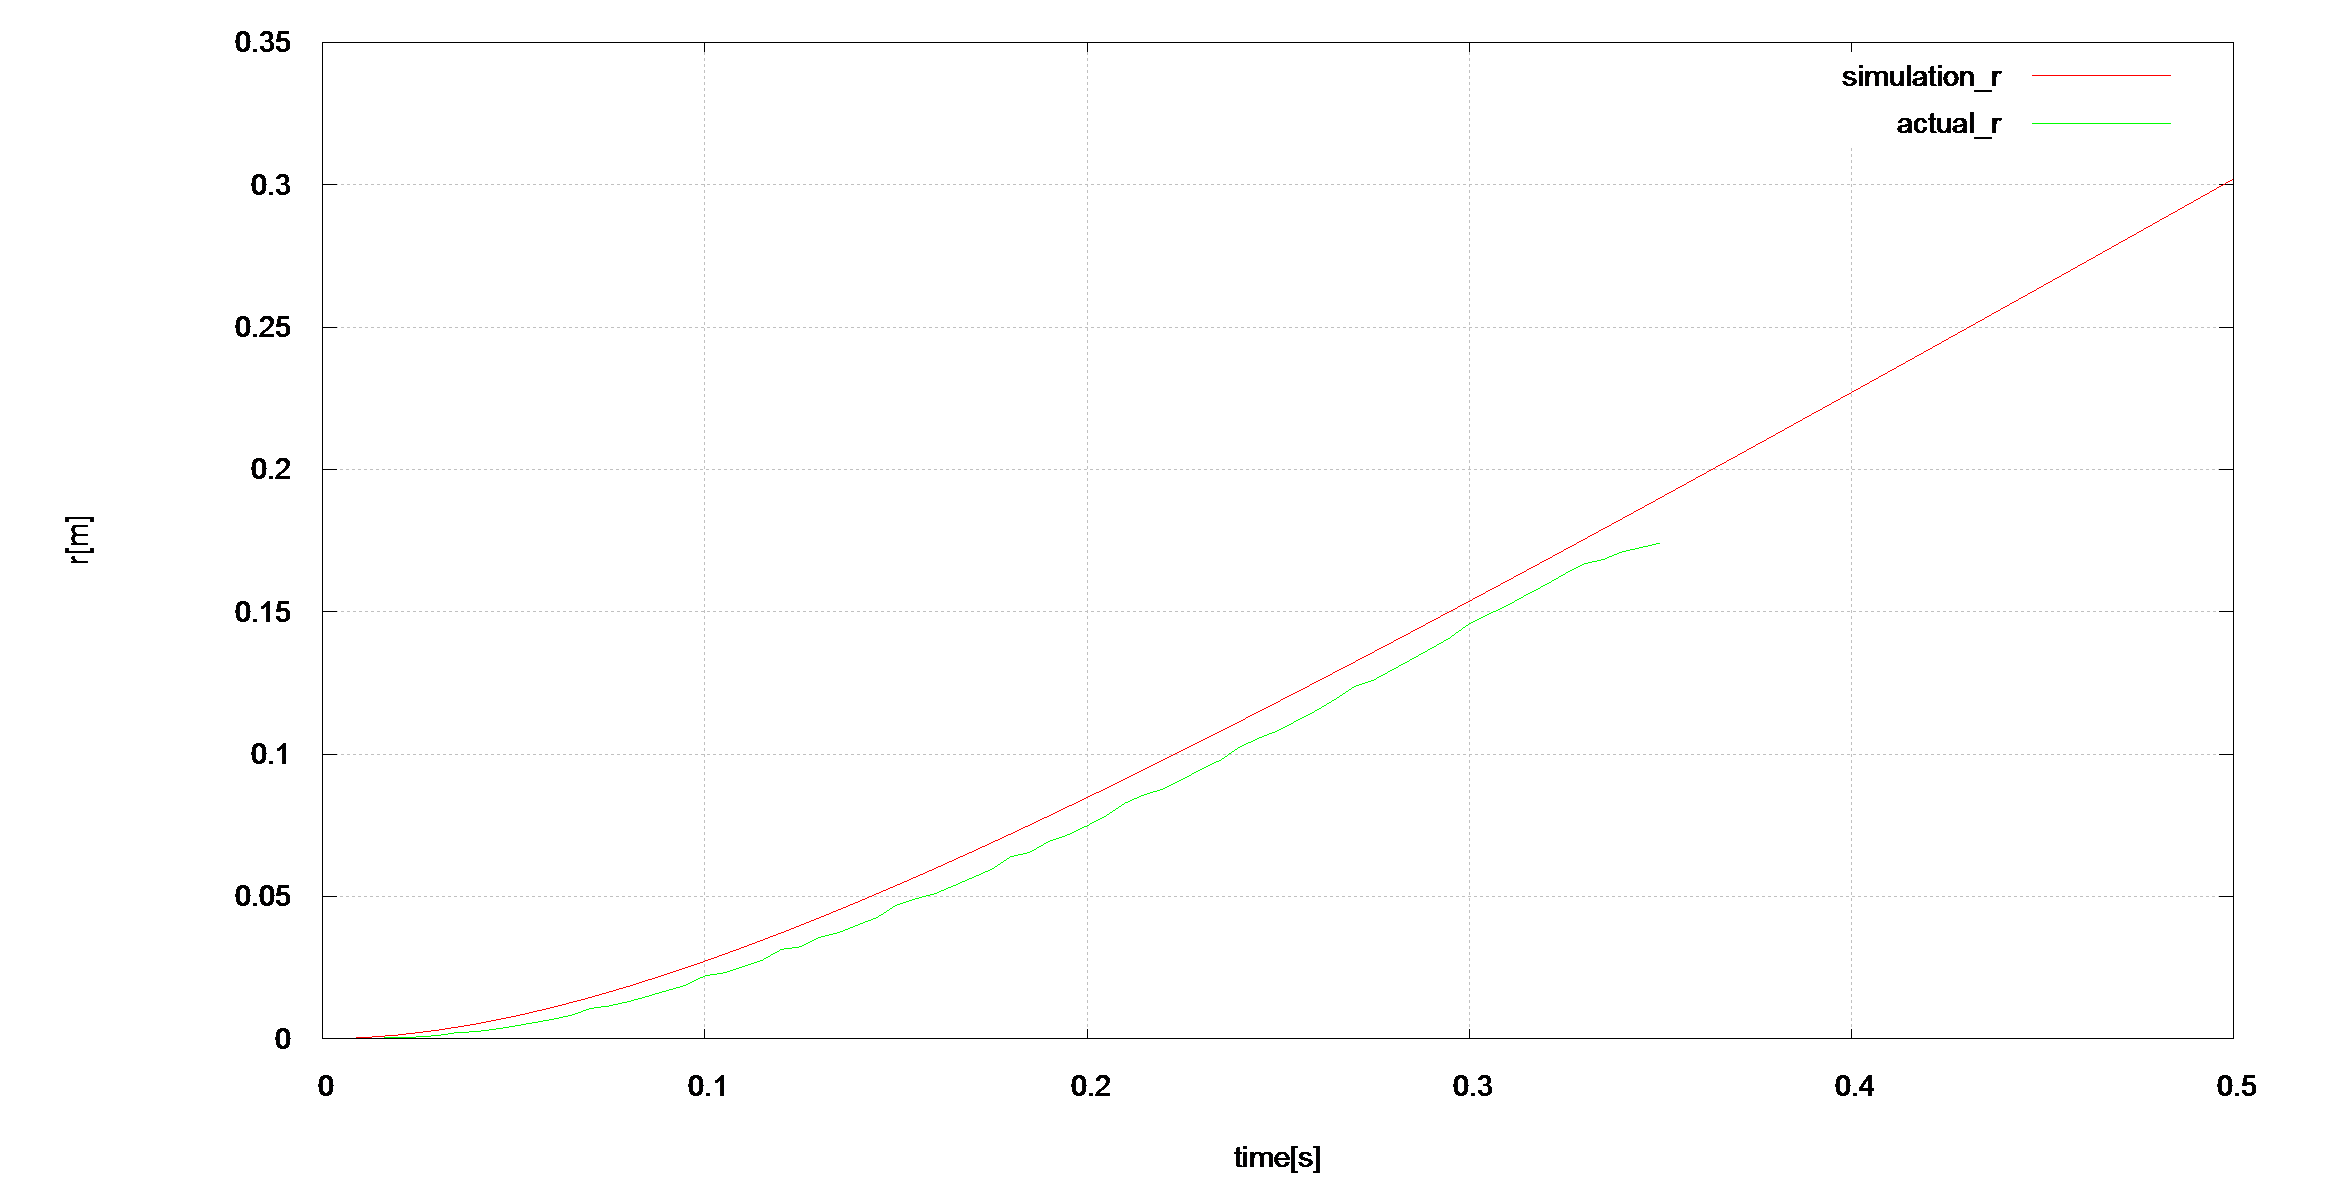
\includegraphics[width = 1.0 \linewidth]{step15.eps}
			\caption{入力電圧15VにおけるMとfの検証}
			\label{fig:step15}
		\end{center}
	\end{figure}
	
	
	\subsection{$J$と$c$の検証}
	\begin{figure}[htbp]
		\begin{center}
			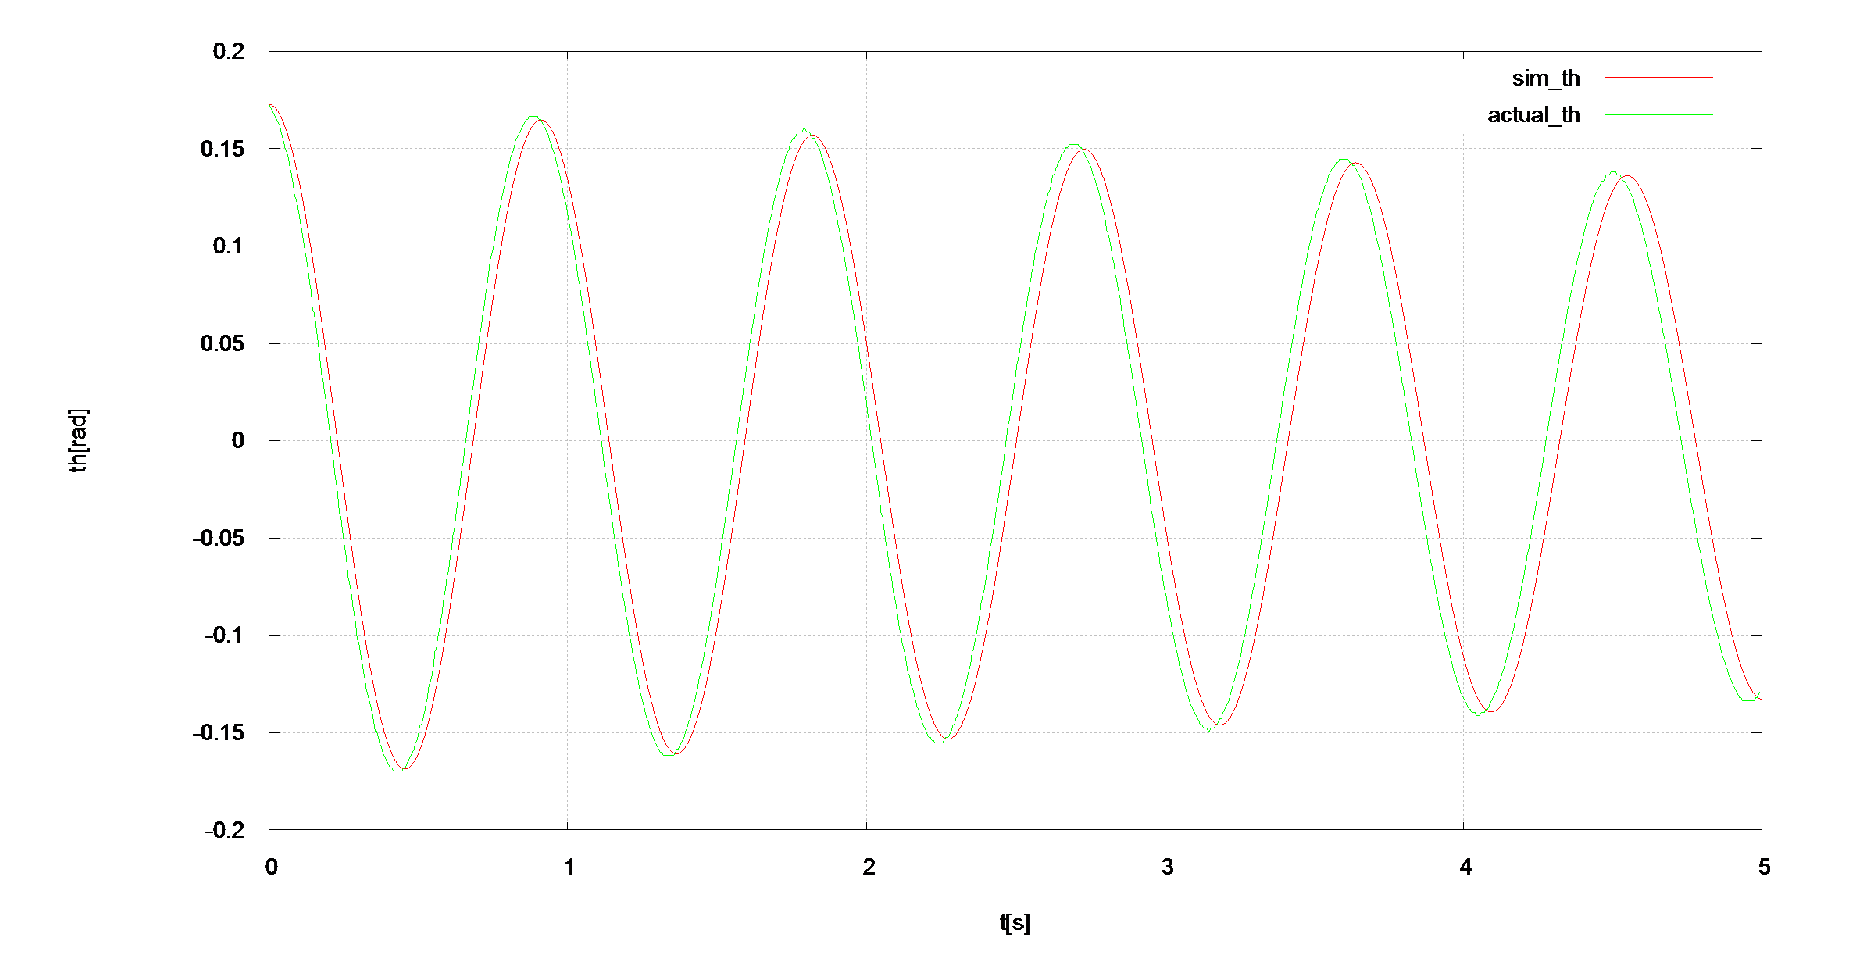
\includegraphics[width = 1.0 \linewidth]{freePendulum.eps}
			\caption{測定した$J$と$c$を用いたシミュレーションと実験データ}
			\label{fig:Jc}
		\end{center}
	\end{figure}
	図\ref{fig:Jc}、は測定した$J$と$c$を用いた自由振動のシミュレーションのデータと、
	実際の自由振動の実験結果を重ね合わせたグラフである。


<<<<<<< HEAD
\section{パラメータの検証}
求めたパラメータを以下に示す。

\begin{table}[hbtp]
	\begin{center}
		\caption{物理パラメータ}
		\medskip
		\begin{tabular}{|ll|l|} \hline
			$m$ & $[\mathrm{kg}]$ & 0.038 \\ \hline
			$l$ & $[\mathrm{m}]$ & 0.12 \\ \hline
			$M(\rm{Step})$ & $[\mathrm{kg}]$ & 1.001 \\ \hline
			$f(\rm{Step})$ & $[\mathrm{kg/s}]$ & 9.67 \\ \hline
			$M(\rm{Feedback})$ & $[\mathrm{kg}]$ & 1.51 \\ \hline
			$f(\rm{Feedback})$ & $[\mathrm{kg/s}]$ & 16.5 \\ \hline
			$J$ & $[\mathrm{kgm^2}]$ & 3.9e-4 \\ \hline
			$c$ & $[\mathrm{kgm^2/s}]$ & 9.82e-5 \\ \hline
			$a$ & $[\mathrm{N/V}]$ & 0.49 \\ \hline
			$c_1$ & $[\mathrm{V/m}]$ & 1.0 \\ \hline
			$c_2$ & $[\mathrm{V/rad}]$ & 1.0 \\ \hline
			$g$ & $[\mathrm{m/s^2}]$ & 9.8 \\ \hline
		\end{tabular}
	\end{center}
\end{table}

\begin{figure}[htbp]
	\begin{center}
		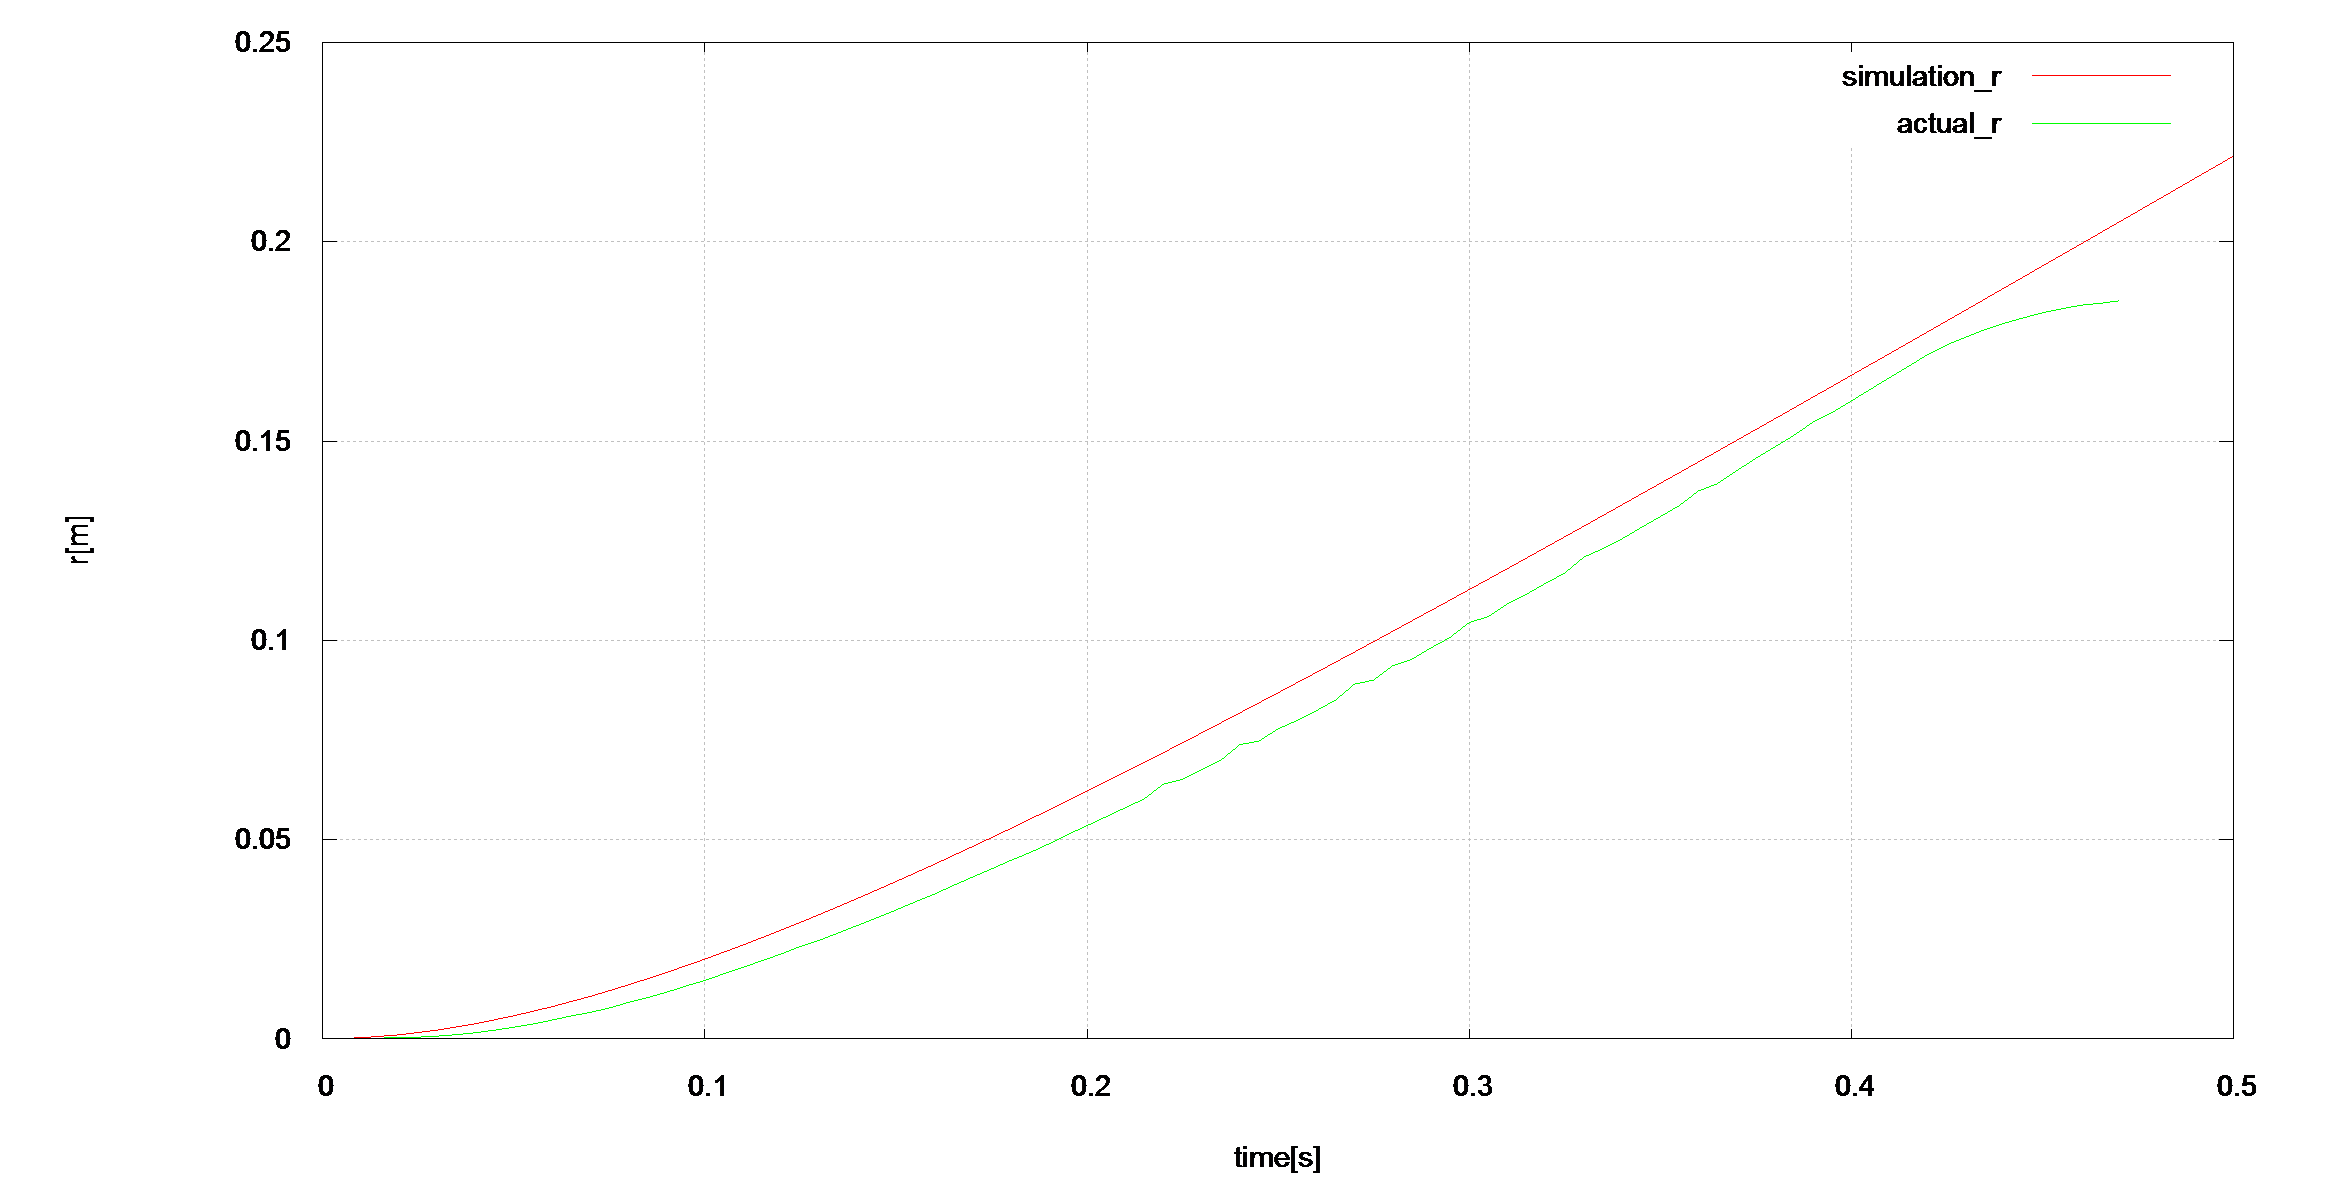
\includegraphics[width = 1.0 \linewidth]{step11.eps}
		\caption{入力電圧11VにおけるMとfの検証}
		\label{fig:入力電圧11VにおけるMとfの検証}
	\end{center}
\end{figure}

=======
>>>>>>> c75b7fa605d82ac36c3c13370dbdcf9029f17b03
=======
>>>>>>> 1393f4f07a5b2b89c455e47e2d9b68edaf40a925
\chapter{制御系設計}
	\section{特性解析(未完成)}
		前章までに、倒立振子系の数式モデルおよび物理パラメータを求めることができた。よって、倒立振子の状態空間表現における行列$A,B,C$の値を計算することができる。$A,B,C$の値はそれぞれ、
		\begin{eqnarray*}
			A = \left[
			\begin{array}{rrrr}
				0 & 0 & 1 & 0\\
				0 & 0 & 0 & 1\\
				0 & 0 & 0 & 0\\
				0 & 0 & 0 & 0
			\end{array}
			\right],\,
			B = \left[
			\begin{array}{c}
				0 \\
				0 \\
				0 \\
				0
			\end{array}
			\right],\,
			C = \left[
			\begin{array}{cccc}
				1 &  0 & 0 & 0\\
				0 &  1 & 0 & 0
			\end{array}
			\right]
		\end{eqnarray*}
		のようになった。この値を用いて特性解析を行う。
		
		まず、安定性については、$A$の固有値の実部を調べればよい。
		
		次に、可制御については$(A,B)$に対し可制御性行列
		\begin{eqnarray*}
			U_c=
			\left[
				\begin{array}{ccc}
					B , AB , A^2B , … , A^{n-1}B
				\end{array}
			\right]
		\end{eqnarray*}
		を計算し、行列$N_c$が行フルランクならば可制御、そうでなければ不可制御と判定する。ただし、$n$はシステムの次数(倒立振子系の場合は$n=4$)である。よって、可制御性を調べたい行列は、
		\begin{eqnarray*}
			N_c 
			=
			\left[
				\begin{array}{cccc}
					B & AB & A^2B & A^3B
				\end{array}
			\right]
		\end{eqnarray*}
		となる。
		
		次に、可観測性については、$(A^T,C^T)$に対し可観測性行列
		
		\begin{eqnarray*}
			U_o = \left[
			\begin{array}{c}
				C\\
				CA\\
				CA^2\\
				\vdots\\
				CA^{n-1}
			\end{array}
			\right]
		\end{eqnarray*}
		を計算し、行列$U_o$のランクがシステムの次数と等しいなら可観測、そうでなければ不可観測と判断すればよい。	ただし、$n$はシステムの次数$(倒立振子系の場合n=4)$である。よって、可観測性を調べたい行列$N_o$は
		
		\begin{eqnarray*}
			N_o = \left[
			\begin{array}{c}
				C\\
				CA\\
				CA^2\\
				CA^{3}
			\end{array}
			\right]
		\end{eqnarray*}
		となる。
	\section{制御システムの構成(未完成)}
	
		\begin{figure}[htbp]
			\begin{center}
				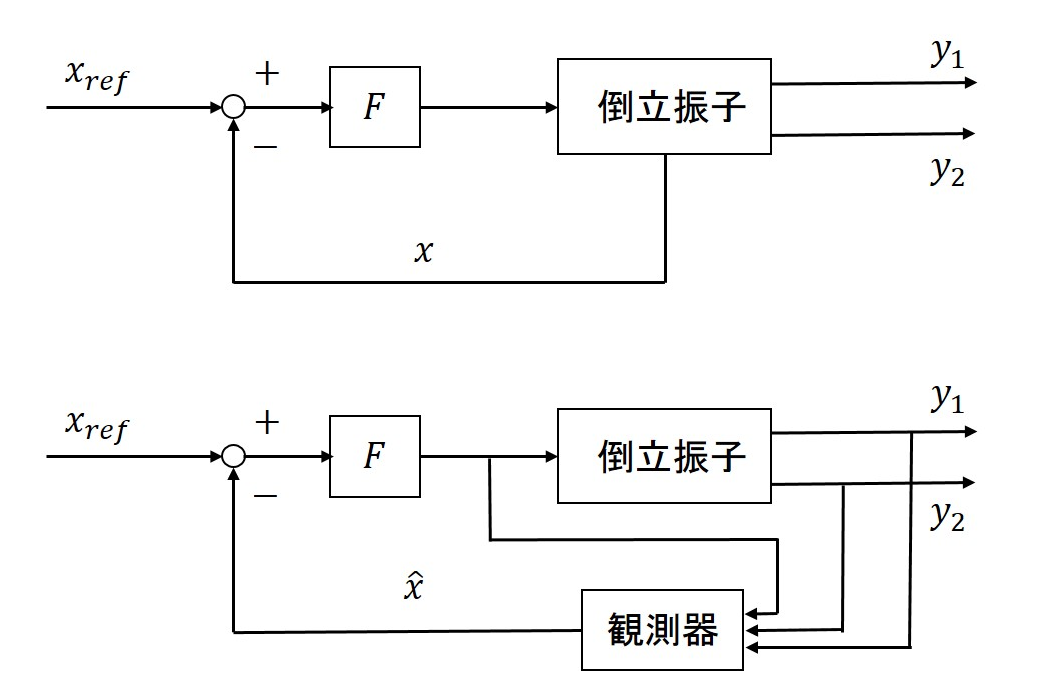
\includegraphics[width = 0.6 \linewidth]{system.eps}
				\caption{制御システムの構成}
				\label{fig:制御システムの構成}
			\end{center}
		\end{figure}
		図\ref{fig:制御システムの構成}に、倒立振子系に対する制御システムの構成を示す。制御則は
		\begin{eqnarray*}
			u = -F(x-x_{ref})
		\end{eqnarray*}
		ただし
		\begin{eqnarray*}
			x_{ref} = \left[
			\begin{array}{c}
				y_c\\
				0\\
				0\\
				0
			\end{array}
			\right]
		\end{eqnarray*}
		である。ここで、$y_c$は指定された倒立位置を表している。また、状態$x$は直接には得られないので$(\dot{r},\dot{\theta}の検出器はない)$
		\begin{eqnarray*}
			\hat{x} \to x \,\,\, (t \to \infty)
			\label{eq:xhat,x}
		\end{eqnarray*}
		を満足させる最小次元オブザーバ
		\begin{eqnarray}
			\hat{z} & = & \hat{A}z + \hat{B}y + \hat{J}u
			\label{eq:zhat}\\
			\hat{x} & = & \hat{C}z + \hat{D}y
			\label{eq:xhat}
		\end{eqnarray}
		を用いる。ここで、オブザーバの次数は2である。したがって、設計すべき制御システムのパラメータは、
		つぎのものである。
		\begin{description}
			\item  1゜$F(1\times4)$
			\item  2゜$\hat{A}(2\times2),\hat{B}(2\times2),\hat{J}(2\times1),
					\hat{C}(4\times2),\hat{D}(4\times2)$
		\end{description}
		
	\section{$F$の設計}
		$F$は、システムを安定化する状態フィードバック
		\begin{eqnarray}
			u = -Fx
			\label{eq:u}
		\end{eqnarray}
		として求めればよい。
		さて、(\ref{eq:u})式をLQ問題の解として得るために、2次形式評価関数
		\begin{eqnarray}
			J &=& \int_0^\infty (x^TQx + Ru^2) dt
			\label{eq:J}\\
			Q &=& \rm{diag}(q^2_1,q^2_2,q^2_3,q^2_4), \,\,\, R = 1
			\label{eq:Q,R}
		\end{eqnarray}
		を考える。ただし、$\rm{diag}(\ldots)$は、対角行列を表す。これは
		\begin{eqnarray}
			J &=& \int_0^\infty (q^2_1r^2 + q^2_2\theta^2 + q^2_3\dot{r}^2 + q^2_4
			\dot{\theta}^2 + u^2) dt
		\end{eqnarray}
		のように表されることから、$q_1,q_2,q_3,q_4$は台車位置$r$、振子角度$\theta$、台車速度$\dot{r}$、振子角速度$\dot{\theta}$の間のバランスをとる重み係数である。
		
		(\ref{eq:J})-(\ref{eq:Q,R})を最小にする(\ref{eq:u})における$F$は、リカッチ方程式
		\begin{eqnarray*}
			A^TP + PA - PBR^{-1}B^TP + Q = 0
		\end{eqnarray*}
		の解$P > 0$を求めて
		\begin{eqnarray*}
			F = R^{-1}B^TP
		\end{eqnarray*}
		のように与えられる。
	
	\section{$\hat{A}$,$\hat{B}$,$\hat{J}$,$\hat{C}$,$\hat{D}$の設計}
		オブザーバ(\ref{eq:zhat})-(\ref{eq:xhat})が(\ref{eq:xhat,x})式を満足するための十分条件は、ある行列$U(1\times4)$が存在して
		\begin{eqnarray*}
			UA & = & \hat{A}U + \hat{B}C\\
			UB & = & \hat{J}\\
			I  & = & \hat{C}U + \hat{D}C
		\end{eqnarray*}
		かつ$\hat{A}$が安定行列であることである。これらの条件を満足する、最も代表的なオブザーバの
		設計法は、Gopinathによって提案されたものである。
		
	\section{離散化}
		コントローラは連続時間で記述された(\ref{eq:u})式と(\ref{eq:zhat})-(\ref{eq:xhat})式で与えられるが、計算機制御のためには
		これらを離散時間で記述しなければならない。いま、サンプリング間隔を$\Delta$とすると、
		その結果が次のように与えられる。
		\begin{eqnarray*}
			u[k]       & = & -F\hat{x}[k]\\
			z[k+1]     & = & \hat{A}_dz[k] + \hat{B}_dy[k] + \hat{J}_du[k]\\
			\hat{x}[k] & = & \hat{C}_dz[k] + \hat{D}_dy[k]
		\end{eqnarray*}
		ただし、$k = 0,1,\cdots$であり
		\begin{eqnarray*}
			\left[
				\begin{array}{cc}
					\hat{A}_d & \left[\begin{array}{cc} \hat{B}_d & \hat{J}_d \end{array}
					\right]\\
					0 & I_3
				\end{array}
			\right]
			=
			\exp{
				\left(
					\Delta
					\left[
					\begin{array}{cc}
						\hat{A} & \left[\begin{array}{cc} \hat{B} & \hat{J} \end{array}
						\right]\\
						0 & 0
					\end{array}
					\right]
				\right)
			}
		\end{eqnarray*}
		
	\section{振り上げ制御}	
		台車と振子の運動方程式は
		\begin{eqnarray}
			(M + m)\ddot{r} + ml\cos\theta\ddot{\theta} &=& -f\dot{r} + ml\sin\theta\ddot{\theta}^{2} + au \label{eq:swing1}\\
			ml\cos\theta\ddot{r} + (J + ml^2)\ddot{\theta} &=& mgl\sin\theta - c\dot{\theta} \label{eq:swing2}
		\end{eqnarray}
		で与えられる。振子が垂直上向きのときを基準とする振子の力学的エネルギーは、
		\begin{equation}
			E = \frac{1}{2}(J + ml^2){\dot{\theta}}^2 + mgl(\cos\theta - 1)
		\end{equation}
		で与えられる。また、エネルギーの時間微分は
		\begin{equation}
			\frac{dE}{dt} = (J + ml)\theta\ddot{\theta} - mgl\dot{\theta}\sin\theta \label{eq:swing4}
		\end{equation}
		振り上げ制御のために,次の制御側を用いる。
		\begin{eqnarray}
			u &=& \frac{1}{a}(f\dot{r} - ml\sin\theta\dot{\theta}^{2} + ml\cos\theta\ddot{\theta} + (M + m)v) \label{eq:swing5}\\
			v &=& -\frac{c\dot{\theta}}{ml\cos\theta} + k(E-E_{0}){\rm sign}(\dot\theta\cos\theta) \label{eq:swing6}
		\end{eqnarray}
		ただし、signは符号関数であり,引数の値が負のとき$-1$、引数の値が正のとき$1$、引数の値が$0$のとき$0$となる。
		(\ref{eq:swing5})式を(\ref{eq:swing1})式に代入すると、
		\begin{equation}
			\ddot{r} = v \label{eq:swing7}
		\end{equation}
		を得る。(\ref{eq:swing7})式と(\ref{eq:swing6})式を(\ref{eq:swing2})式に代入すると、
		\begin{equation}
			(J + ml^2)\ddot{\theta} = mgl\sin\theta - ml\cos\theta(k(E-E_{0}){\rm sign}(\dot{\theta}\cos\theta))
		\end{equation}
		を得る。この式を(\ref{eq:swing4})式に代入すると
		\begin{eqnarray*}
			\frac{dE}{dt} 
			&=&-ml\dot\theta\cos\theta(k(E-E_{0})\rm{sign}(\dot{\theta}\cos\theta))\\
			&=&-mlk(E-E_{0})\rm{sign}(\dot{\theta}\cos\theta)(\dot{\theta}\cos\theta)
		\end{eqnarray*}
		リアプノフ関数の候補として
		\begin{equation}
			V = \frac{(E - E_{0})^{2}}{2} \geq 0
		\end{equation}
		を考える。$V$の時間微分を求める
		\begin{eqnarray*}
			\frac{dV}{dt} &=& (E - E_{0})\frac{dE}{dt}\\
			&=&  -mlk(E-E_{0})^{2}{\rm sign}(\dot{\theta}\cos\theta))\dot{\theta}(\cos\theta)  \le 0
		\end{eqnarray*}
		これより、$\dot{\theta}\cos\theta\neq0$のとき、$V$は減少し、$0$に収束し、$E$は$E_{0}$に収束する。
		
		実際の制御では、台車の加速度目標$v$を制限し、
		\begin{eqnarray}
			u &=& \frac{1}{a}(f\dot{r} - ml\sin\theta\dot{\theta}^{2} + ml\cos\theta\ddot{\theta} + (M + m)v)\\
			v &=& -\frac{c\dot{\theta}}{ml\cos\theta} + {\rm sat}_{ng}(k(E-E_{0}){\rm sign}(\dot\theta\cos\theta))
		\end{eqnarray}
<<<<<<< HEAD
		とする。ただし、$\rm{sat}$は最小値が$-ng$、最大値が$ng$の飽和関数である。$n$は重力加速度(垂直下向き)と台車の加速度(水平方向)の比である。また、$k$を大きくすると、早く$E$が$E_{0}$に収束する。
=======
		とする。ただし、$\roman{sat}$は最小値が$-ng$、最大値が$ng$の飽和関数である。$n$は重力加速度(垂直下向き)と台車の加速度(水平方向)の比である。また、$k$を大きくすると、早く$E$が$E_{0}$に収束する。
>>>>>>> 1393f4f07a5b2b89c455e47e2d9b68edaf40a925
		
\chapter{シミュレーション}
	\section{安定化制御}
	\section{振り上げ制御}

\chapter{実験}
	\section{実験装置}
	
	\section{安定化制御}
		\subsection{シミュレーションと実験データの比較}
			表\ref{tb:QPTtable}の重み行列$Q$の3種類、オブザーバの極$P$の2種類、サンプリング周期$dt$の2種類、これらの組み合わせの
			計12種類のパラメータについてシミュレーションの結果と実際の実験データとの比較を行った。
			比較に用いたパラメータの表を表\ref{tb:QPTtable}に示す。\\
			\begin{table}[htbp]
				\begin{center}
					\caption{重み行列、オブザーバの極、サンプリング周期の組み合わせ12通り}
					\medskip
					\begin{tabular}{|c|c|c|c|} \hline
						& 重み行列$Q$ & オブザーバの極$P$ & サンプリング周期$dt$ \\ \hline\hline
						case01 &$Q_1:\rm{diag}(1.0E+6,1.0E+5,1,1)$ &$P_1:(-23,-23)$ & ${dt}_2:0.01$ \\\hline
						case02 &$Q_1:\rm{diag}(1.0E+6,1.0E+5,1,1)$ &$P_2:(-50,-50)$ & ${dt}_2:0.01$ \\\hline
						case03 &$Q_1:\rm{diag}(1.0E+6,1.0E+5,1,1)$ &$P_1:(-23,-23)$ & ${dt}_1:0.005$ \\\hline
						case04 &$Q_1:\rm{diag}(1.0E+6,1.0E+5,1,1)$ &$P_2:(-50,-50)$ & ${dt}_1:0.005$ \\\hline
						case05 &$Q_2:\rm{diag}(1.0E+5,1.0E+6,1,1)$ &$P_1:(-23,-23)$ & ${dt}_1:0.005$ \\\hline
						case06 &$Q_2:\rm{diag}(1.0E+5,1.0E+6,1,1)$ &$P_2:(-50,-50)$ & ${dt}_1:0.005$ \\\hline
						case07 &$Q_2:\rm{diag}(1.0E+5,1.0E+6,1,1)$ &$P_1:(-23,-23)$ & ${dt}_2:0.01$  \\\hline
						case08 &$Q_2:\rm{diag}(1.0E+5,1.0E+6,1,1)$ &$P_2:(-50,-50)$ & ${dt}_2:0.01$  \\\hline
						case09 &$Q_3:\rm{diag}(1.0E+6,1.0E+6,1,1)$ &$P_1:(-23,-23)$ & ${dt}_2:0.01$  \\\hline
						case10 &$Q_3:\rm{diag}(1.0E+6,1.0E+6,1,1)$ &$P_2:(-50,-50)$ & ${dt}_2:0.01$  \\\hline
						case11 &$Q_3:\rm{diag}(1.0E+6,1.0E+6,1,1)$ &$P_1:(-23,-23)$ & ${dt}_1:0.005$  \\\hline
						case12 &$Q_3:\rm{diag}(1.0E+6,1.0E+6,1,1)$ &$P_2:(-50,-50)$ & ${dt}_1:0.005$  \\\hline
					\end{tabular}
					\label{tb:QPTtable}
				\end{center}
			\end{table}
		
		シミュレーションと実験データを重ねたグラフを図\ref{fig:case1}-\ref{fig:case12}に示す。
		
		%Q1
		\begin{figure}[htbp]
			\centering
			\subfigure[台車]{
				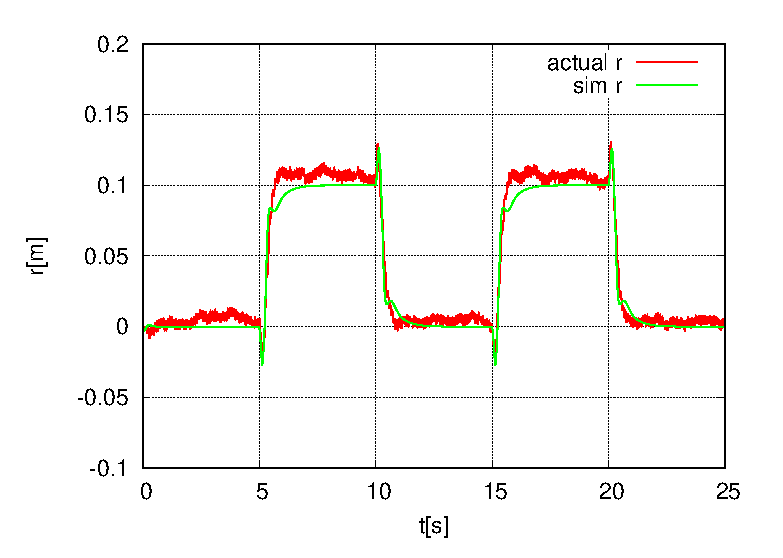
\includegraphics[clip,width=0.45\linewidth]{case1_r.eps}
				\label{1_r}
			}
			\hspace{5mm}
			\subfigure[振子]{
				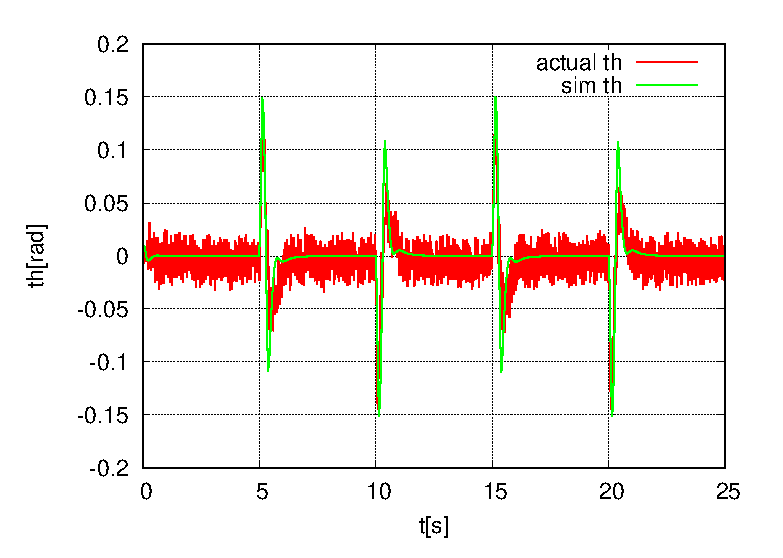
\includegraphics[clip,width=0.45\linewidth]{case1_th.eps}
				\label{1_th}
			}
			\caption{${\rm Q_1,obs_1,dt_1}$のシミュレーションと実験結果}\label{case1}
		\end{figure}
		
		
		\begin{figure}[htbp]
			\centering
			\subfigure[台車]{
				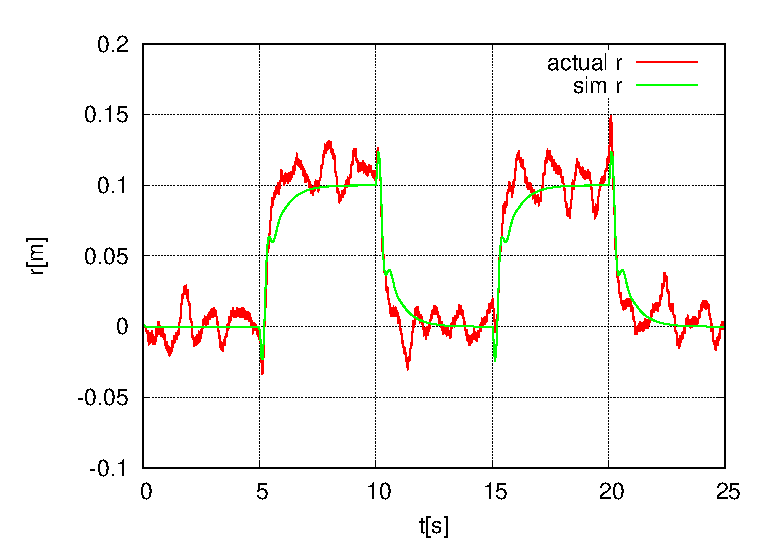
\includegraphics[clip,width=0.45\linewidth]{case2_r.eps}
				\label{2_r}
			}
			\hspace{5mm}
			\subfigure[振子]{
				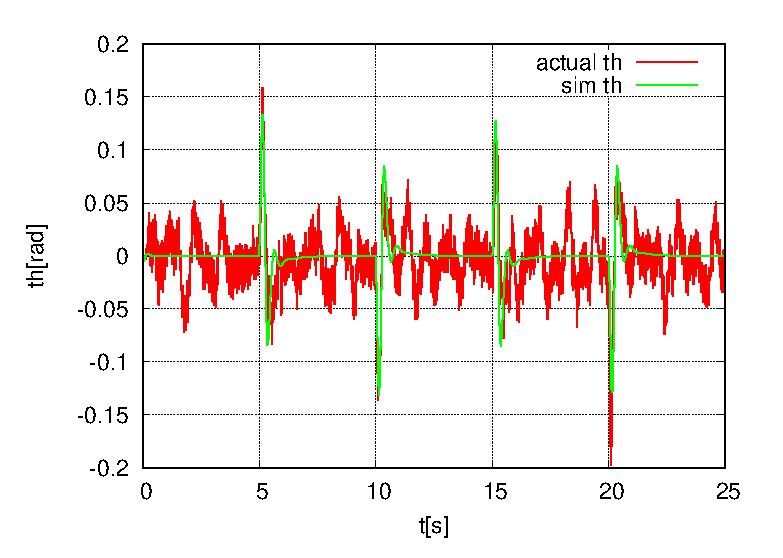
\includegraphics[clip,width=0.45\linewidth]{case2_th.eps}
				\label{2_th}
			}
			\caption{${\rm Q_1,obs_1,dt_2}$のシミュレーションと実験結果}\label{case2}
		\end{figure}
		
		
		\begin{figure}[htbp]
			\centering
			\subfigure[台車]{
				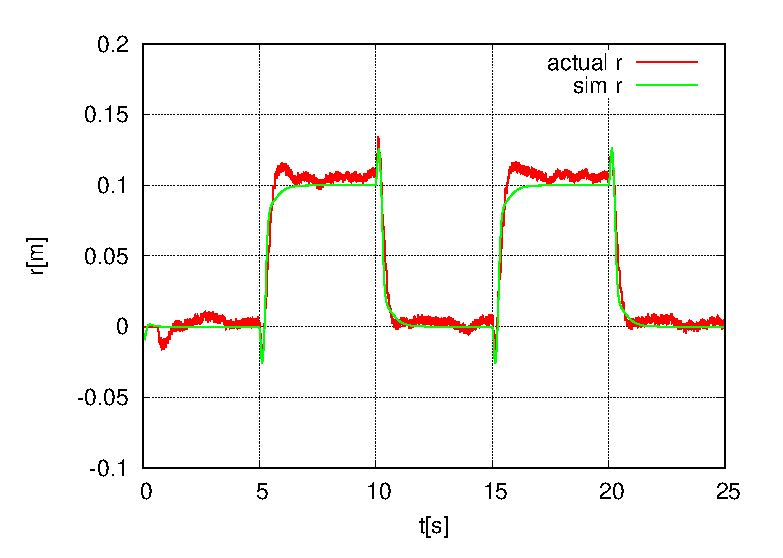
\includegraphics[clip,width=0.45\linewidth]{case3_r.eps}
				\label{3_r}
			}
			\hspace{5mm}
			\subfigure[振子]{
				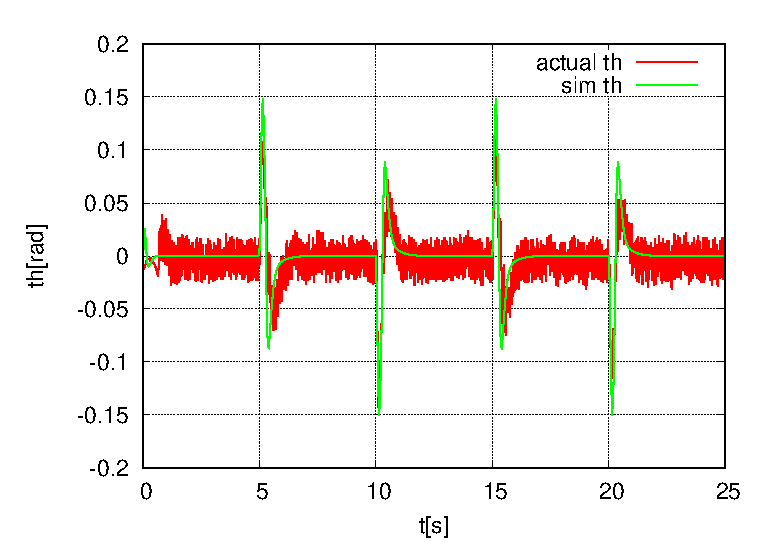
\includegraphics[clip,width=0.45\linewidth]{case3_th.eps}
				\label{3_th}
			}
			\caption{${\rm Q_1,obs_2,dt_1}$のシミュレーションと実験結果}\label{case3}
		\end{figure}
		
		
		\begin{figure}[htbp]
			\centering
			\subfigure[台車]{
				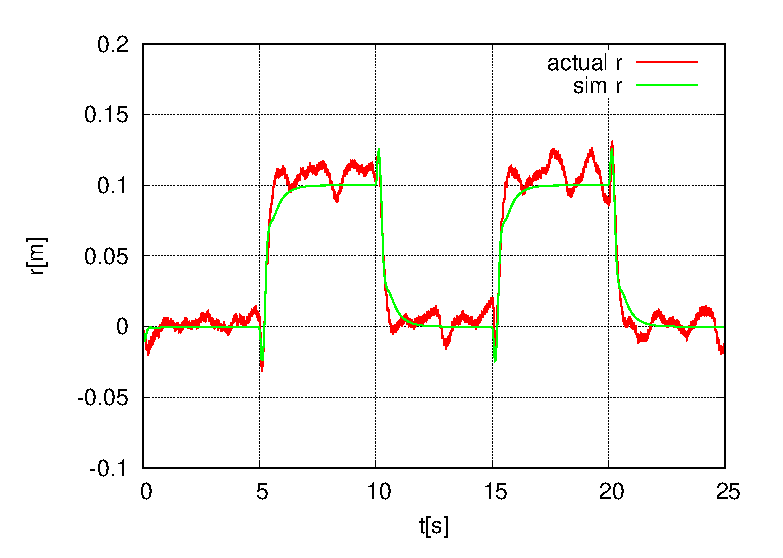
\includegraphics[clip,width=0.45\linewidth]{case4_r.eps}
				\label{4_r}
			}
			\hspace{5mm}
			\subfigure[振子]{
				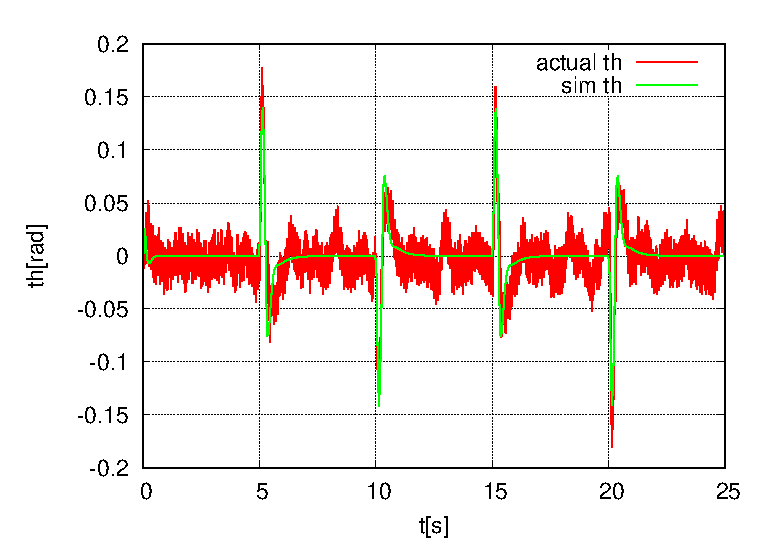
\includegraphics[clip,width=0.45\linewidth]{case4_th.eps}
				\label{4_th}
			}
			\caption{${\rm Q_1,obs_2,dt_2}$のシミュレーションと実験結果}\label{case4}
		\end{figure}
		%Q1
		
		%Q2
		
		\begin{figure}[htbp]
			\centering
			\subfigure[台車]{
				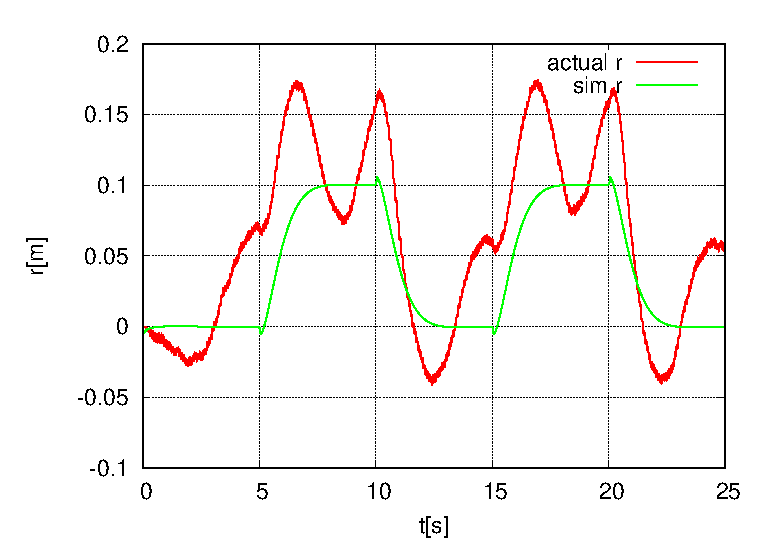
\includegraphics[clip,width=0.45\linewidth]{case5_r.eps}
				\label{5_r}
			}
			\hspace{5mm}
			\subfigure[振子]{
				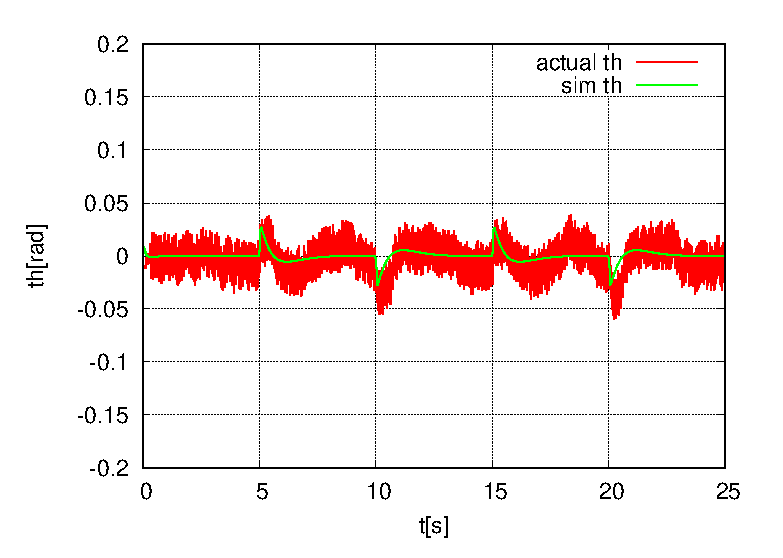
\includegraphics[clip,width=0.45\linewidth]{case5_th.eps}
				\label{5_th}
			}
			\caption{${\rm Q_2,obs_1,dt_1}$のシミュレーションと実験結果}\label{case5}
		\end{figure}
		
		
		\begin{figure}[htbp]
			\centering
			\subfigure[台車]{
				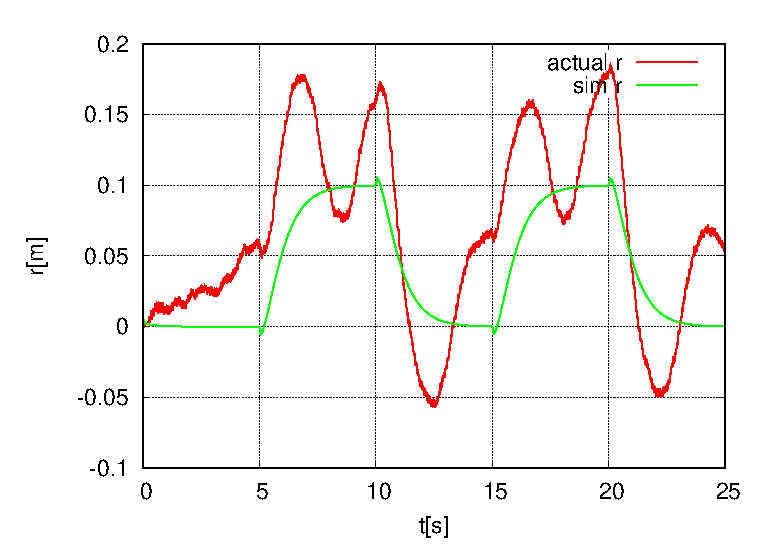
\includegraphics[clip,width=0.45\linewidth]{case6_r.eps}
				\label{6_r}
			}
			\hspace{5mm}
			\subfigure[振子]{
				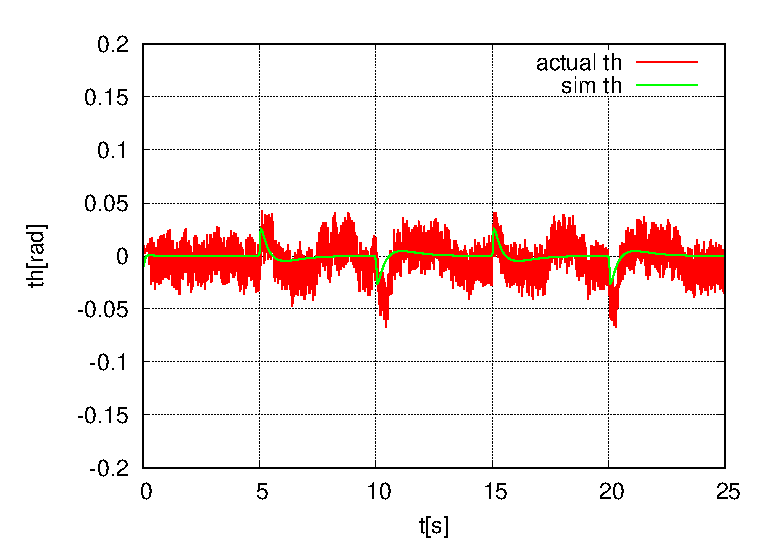
\includegraphics[clip,width=0.45\linewidth]{case6_th.eps}
				\label{6_th}
			}
			\caption{${\rm Q_2,obs_1,dt_2}$のシミュレーションと実験結果}\label{case6}
		\end{figure}
		
		
		\begin{figure}[htbp]
			\centering
			\subfigure[台車]{
				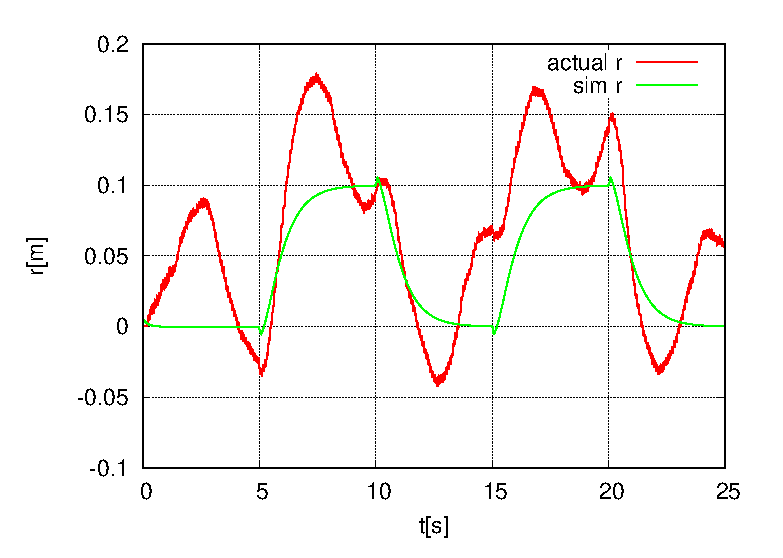
\includegraphics[clip,width=0.45\linewidth]{case7_r.eps}
				\label{7_r}
			}
			\hspace{5mm}
			\subfigure[振子]{
				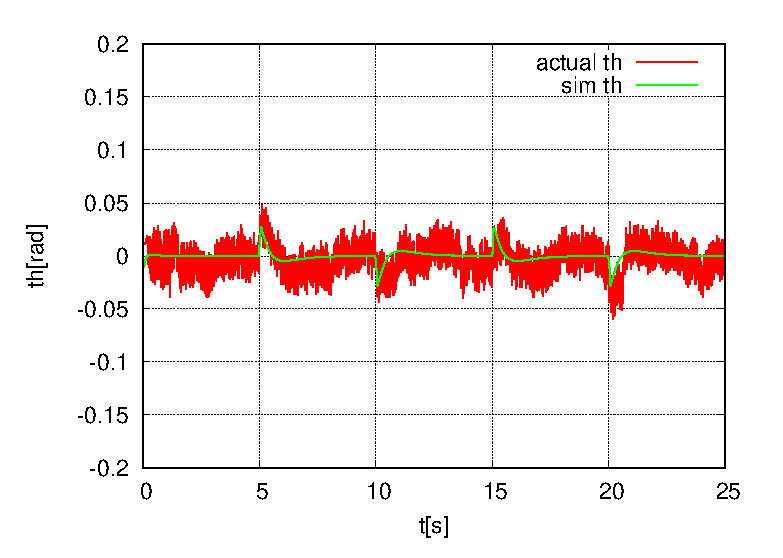
\includegraphics[clip,width=0.45\linewidth]{case7_th.eps}
				\label{7_th}
			}
			\caption{${\rm Q_2,obs_2,dt_1}$のシミュレーションと実験結果}\label{case7}
		\end{figure}
		
		
		\begin{figure}[htbp]
			\centering
			\subfigure[台車]{
				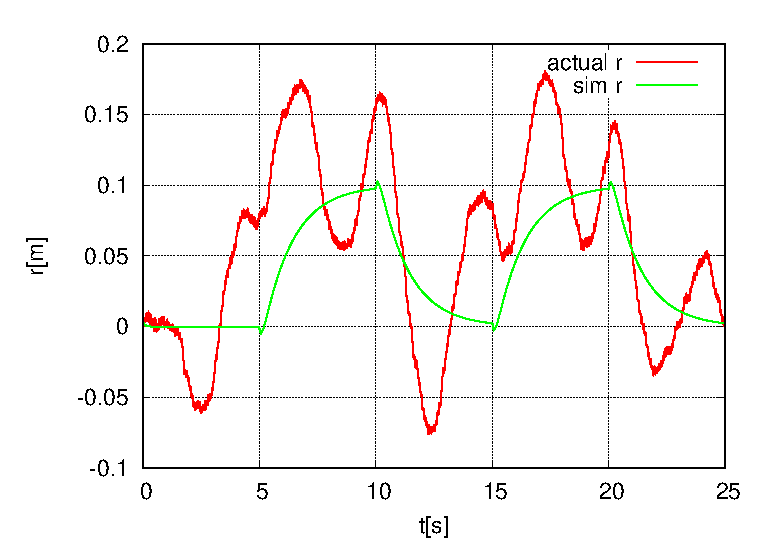
\includegraphics[clip,width=0.45\linewidth]{case8_r.eps}
				\label{8_r}
			}
			\hspace{5mm}
			\subfigure[振子]{
				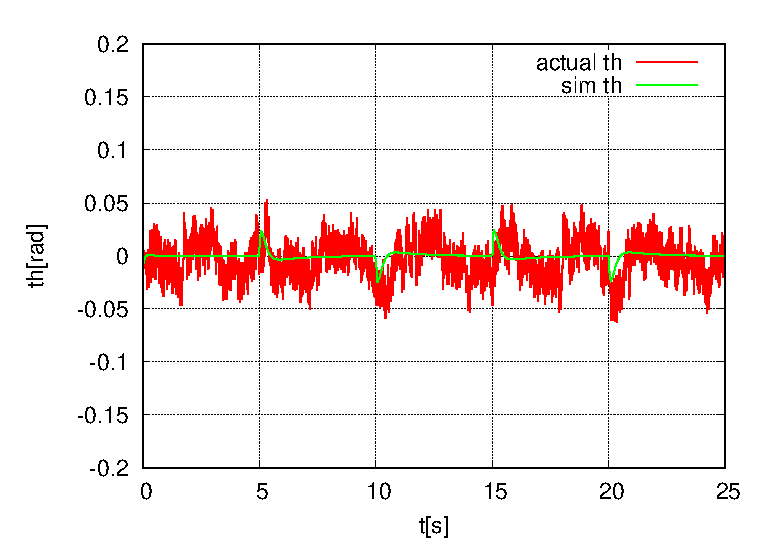
\includegraphics[clip,width=0.45\linewidth]{case8_th.eps}
				\label{8_th}
			}
			\caption{${\rm Q_2,obs_2,dt_2}$のシミュレーションと実験結果}\label{case8}
		\end{figure}
		%Q2
		
		%Q3
		\begin{figure}[htbp]
			\centering
			\subfigure[台車]{
				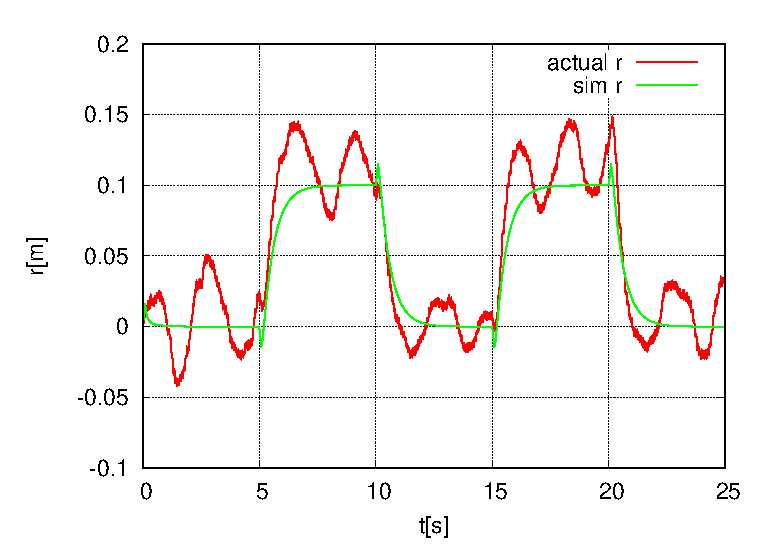
\includegraphics[clip,width=0.45\linewidth]{case9_r.eps}
				\label{9_r}
			}
			\hspace{5mm}
			\subfigure[振子]{
				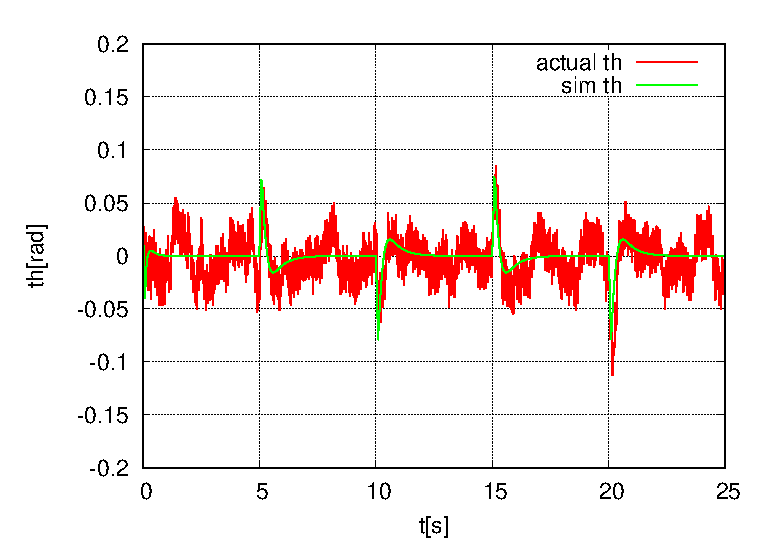
\includegraphics[clip,width=0.45\linewidth]{case9_th.eps}
				\label{9_th}
			}
			\caption{${\rm Q_3,obs_1,dt_1}$のシミュレーションと実験結果}\label{case9}
		\end{figure}
		
		
		\begin{figure}[htbp]
			\centering
			\subfigure[台車]{
				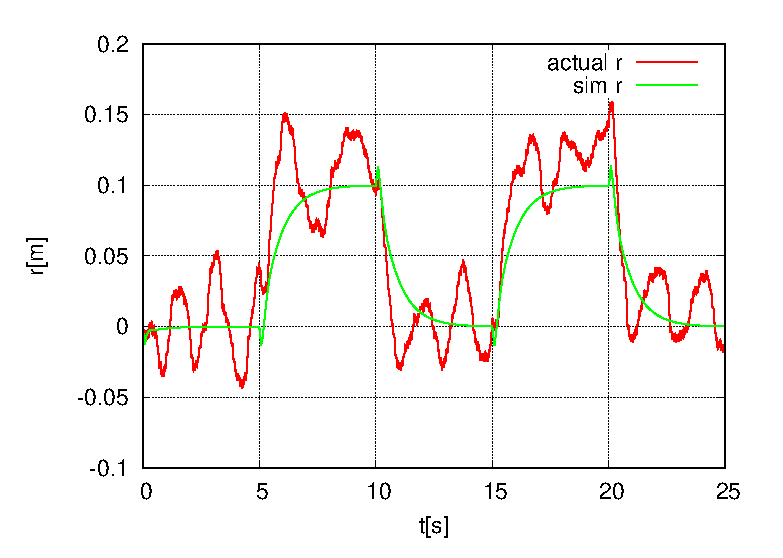
\includegraphics[clip,width=0.45\linewidth]{case10_r.eps}
				\label{10_r}
			}
			\hspace{5mm}
			\subfigure[振子]{
				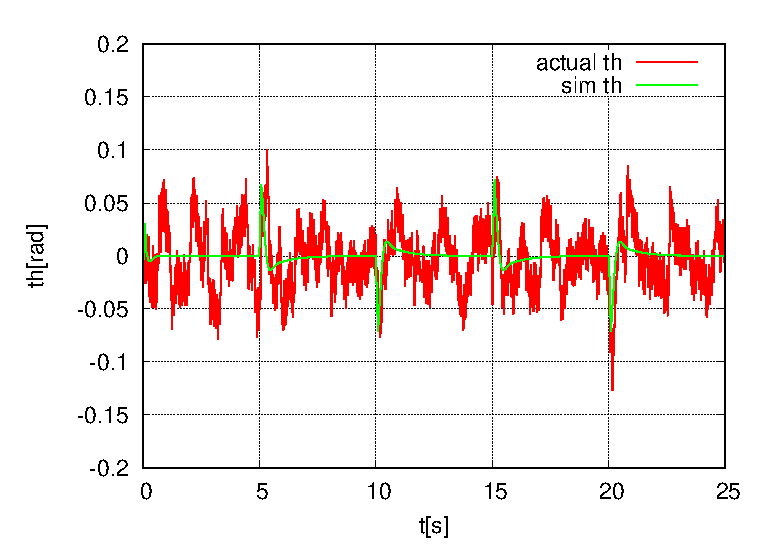
\includegraphics[clip,width=0.45\linewidth]{case10_th.eps}
				\label{10_th}
			}
			\caption{${\rm Q_3,obs_1,dt_2}$のシミュレーションと実験結果}\label{case10}
		\end{figure}
		
		
		\begin{figure}[htbp]
			\centering
			\subfigure[台車]{
				\includegraphics[clip,width=0.45\linewidth]{case11_r.eps}
				\label{11_r}
			}
			\hspace{5mm}
			\subfigure[振子]{
				\includegraphics[clip,width=0.45\linewidth]{case11_th.eps}
				\label{11_th}
			}
			\caption{${\rm Q_3,obs_2,dt_1}$のシミュレーションと実験結果}\label{case11}
		\end{figure}
		
		
		\begin{figure}[htbp]
			\centering
			\subfigure[台車]{
				\includegraphics[clip,width=0.45\linewidth]{case12_r.eps}
				\label{12_r}
			}
			\hspace{5mm}
			\subfigure[振子]{
				\includegraphics[clip,width=0.45\linewidth]{case12_th.eps}
				\label{12_th}
			}
			\caption{${\rm Q_3,obs_2,dt_2}$のシミュレーションと実験結果}\label{case12}
		\end{figure}
		%Q3
	\section{振り上げ制御}
	
	\section{考察}

\chapter{おわりに}

\end{document}